% !TeX root = ../main.tex
% =========================================================================
% CAPÍTULO 2. DISEÑO E IMPLEMENTACIÓN
% Desarrollo íntegro de las prácticas 5, 6, 7 y 8, en ese orden.
% Se adaptan únicamente jerarquía, rutas y etiquetas a la compilación conjunta.
% =========================================================================
\capitulopage{Capítulo II}
\setcounter{section}{2}
\setcounter{subsection}{0}
\phantomsection
\addcontentsline{toc}{section}{Capítulo 2. Diseño e Implementación}
\begin{center}
    {\normalfont\Large\bfseries II. Diseño e Implementación \par}
\end{center}

\begingroup
\setlength{\emergencystretch}{3em}
\providecommand{\estado}[1]{\texttt{#1}}
\providecommand{\nota}[1]{\par\smallskip{\footnotesize\textit{Nota.} #1\par}}
\titleformat{\paragraph}[block]{\normalfont\normalsize\bfseries}{}{0pt}{}
\titlespacing*{\paragraph}{0pt}{10pt}{5pt}
\captionsetup{justification=raggedright,singlelinecheck=off,labelfont=bf,textfont=it,labelsep=newline,skip=6pt}
\renewcommand{\lstlistingname}{Código}
\definecolor{codegray}{rgb}{0.95,0.95,0.95}
\definecolor{codekeyword}{rgb}{0.0,0.2,0.6}
\definecolor{codestring}{rgb}{0.1,0.5,0.1}
\definecolor{codecomment}{rgb}{0.4,0.4,0.4}

\lstset{
inputencoding=utf8,
    extendedchars=true,
    literate=
        {á}{{\'a}}1
        {é}{{\'e}}1
        {í}{{\'i}}1
        {ó}{{\'o}}1
        {ú}{{\'u}}1
        {Á}{{\'A}}1
        {É}{{\'E}}1
        {Í}{{\'I}}1
        {Ó}{{\'O}}1
        {Ú}{{\'U}}1
        {ñ}{{\~n}}1
        {Ñ}{{\~N}}1,
    backgroundcolor=\color{codegray},
    basicstyle=\ttfamily\footnotesize,
    % ... el resto de tu configuración actual
    backgroundcolor=\color{codegray},
    basicstyle=\ttfamily\footnotesize,
    breaklines=true,
    captionpos=b,
    commentstyle=\color{codecomment}\itshape,
    keywordstyle=\color{codekeyword}\bfseries,
    stringstyle=\color{codestring},
    numbers=left,
    numberstyle=\tiny\color{gray},
    stepnumber=1,
    numbersep=8pt,
    showstringspaces=false,
    frame=single,
    framerule=0.5pt,
    rulecolor=\color{black!30}
}


\lstdefinestyle{p8}{basicstyle=\ttfamily\footnotesize,numbers=left,breaklines=true,columns=fullflexible,keepspaces=true,showstringspaces=false}


% INICIO DEL DESARROLLO DE LA PRÁCTICA 5
\subsection{Diseño de la arquitectura y selección tecnológica}
\subsubsection{Retomar la alternativa de solución seleccionada en la Fase 1 como punto de partida del diseño arquitectónico.}
\paragraph*{Definición técnica y naturaleza operativa del artefacto}
PyReach se define como una herramienta de software ejecutable en \textbf{línea de comandos (CLI)} de funcionamiento \textbf{100\% local (\textit{on-premise})}, diseñada específicamente para entornos interpretados compatibles con \textbf{CPython 3.10 o superior}. Su propósito operacional es determinar de manera determinista si las funciones, métodos o símbolos reportados con vulnerabilidades y exposiciones comunes (CVE) en librerías de terceros ---con especial énfasis en dependencias transitivas anidadas en el directorio \texttt{site-\allowbreak packages}--- presentan rutas de ejecución activas desde los puntos de entrada (\textit{entrypoints}) de la aplicación analizada.

A diferencia de las utilidades convencionales de Análisis de Composición de Software (SCA) que realizan un cotejo superficial de versiones en archivos de bloqueo (\texttt{requirements.\allowbreak txt}, \texttt{Pipfile.\allowbreak lock}), PyReach traslada la inspección al \textbf{plano sintáctico y semántico del código fuente en reposo}. Este enfoque contextual resuelve de raíz la causa del problema diagnosticado en \textbf{Lidercom Perú S.A.C.}: el sobrecosto generado por la revisión manual de falsas alertas sobre código muerto en sus microservicios de analítica y procesamiento de lenguaje natural (NLP).

\paragraph*{Premisas, restricciones y requerimientos no funcionales heredados}
La retoma de la Alternativa C traslada al proceso de diseño arquitectónico un conjunto de restricciones normativas, de calidad y de alcance que actúan como condiciones de borde:

\begin{enumerate}
    \item \textbf{Aislamiento estricto de red y soberanía de código (RNF-01 / Control A.8.12 ISO/IEC 27001:2022):} 
    La arquitectura debe estructurarse de modo que el análisis sintáctico, la generación de grafos, la resolución de rutas y la persistencia operen de forma local. Cero bytes (0 bytes) de código fuente, representaciones intermedias o metadatos técnicos pueden abandonar la red corporativa de Lidercom Perú S.A.C., garantizando la confidencialidad de los algoritmos de la empresa.

    \item \textbf{Filtrado determinista de falsas alarmas ($\ge 70\%$, RNF-02):} 
    El motor de alcanzabilidad debe podar las ramas de código no invocadas en librerías de terceros, reduciendo como mínimo en un 70\% las alertas irrelevantes y clasificando cada hallazgo en tres estados deterministas: \textit{Alcanzable}, \textit{Inalcanzable} o \textit{Potencialmente alcanzable}.

    \item \textbf{Eficiencia y rendimiento en integración continua (RNF-03):} 
    Los módulos arquitectónicos deben estar desacoplados para asegurar que el tiempo total de procesamiento (parseo, construcción del grafo y evaluación de caminos) no exceda el umbral de \textbf{45 segundos} sobre repositorios con hasta 50 dependencias directas en hardware local estándar.

    \item \textbf{Interoperabilidad de salida y modo fuera de línea (RNF-04 y RNF-05):} 
    La arquitectura debe integrar un serializador estricto compatible al 100\% con el estándar internacional \textbf{OASIS SARIF v2.1.0}, permitiendo la comunicación nativa con plataformas CI/CD (GitHub Actions, GitLab CI). Asimismo, la correlación de avisos debe resolverse localmente mediante una base de datos embebida \textbf{SQLite 3} sincronizada con el catálogo abierto \textbf{OpenSSF OSV}, habilitando una operatividad 100\% \textit{offline}.

    \item \textbf{Fronteras innegociables de la triple restricción y trade-offs:} 
    En conformidad con los acuerdos de gobernanza de la Fase 1 ---donde el \textbf{Tiempo} es innegociable (8 semanas de desarrollo para la Fase 2) y el \textbf{Costo} está restringido a un presupuesto de S/ 3,500.00---, se excluyen de la arquitectura módulos de análisis dinámico en tiempo de ejecución (DAST), introspección de binarios compilados en C/C++ y herramientas de remediación automática mediante modelos LLM comerciales. Ante constructos dinámicos en Python (\texttt{eval()}, \texttt{exec()}, introspección arbitraria), el sistema aplicará una heurística preventiva de seguridad (\textit{soundness}) sin comprometer el cronograma.
\end{enumerate}

La formalización de estas condiciones técnicas establece la línea base sobre la cual se selecciona el estilo arquitectónico y se definen los componentes desacoplados del sistema en las secciones subsiguientes.


\subsubsection{Elegir el estilo arquitectónico en función de los requerimientos no funcionales priorizados, justificando la elección.}

El diseño arquitectónico de un sistema no debe responder a preferencias subjetivas ni a tendencias tecnológicas transitorias, sino que debe derivarse formalmente de los requerimientos no funcionales (RNF) priorizados y de las restricciones operacionales del entorno donde operará el artefacto \cite{pressman2020software, martin2017cleanarch}. Para la herramienta \textbf{PyReach}, se selecciona una \textbf{Arquitectura en Capas Desacoplada (\textit{Layered Architecture})} estructurada bajo los principios de la Arquitectura Limpia (\textit{Clean Architecture}) \cite{martin2017cleanarch}, complementada internamente con un patrón de procesamiento secuencial por etapas (\textit{Pipes and Filters}) dentro del motor analítico central.

\paragraph*{Evaluación y descarte de estilos arquitectónicos alternativos}
Siguiendo las advertencias metodológicas del curso respecto a evitar la sobreingeniería \cite{torres2026proyecto}, se evaluaron y descartaron los siguientes estilos arquitectónicos:

\begin{itemize}
    \item \textbf{Arquitectura basada en Microservicios distribuidos:} Se descarta por constituir una sobrecomplejidad injustificada para una herramienta orientada a la integración en líneas de comandos (CLI) y entornos de integración continua (CI/CD). La comunicación mediante llamadas remotas (RPC o HTTP REST) introduciría latencia de red innecesaria (vulnerando el límite temporal de 45 segundos del RNF-03), demandaría infraestructura adicional de orquestación (contenedores múltiples o balanceadores) que viola el techo presupuestal de S/ 3,500.00, y elevaría la superficie de ataque en el host corporativo \cite{humble2010continuous, ladisa2023sok}.
    \item \textbf{Arquitectura Monolítica no estructurada (\textit{Scripting} plano):} Se descarta debido a que agrupar el parseo de manifiestos, el recorrido de árboles sintácticos, la persistencia en base de datos y la renderización en consola en un bloque acoplado impide la aplicación de pruebas unitarias automatizadas bajo TDD \cite{myers2011art}, eleva exponencialmente la deuda técnica y obstaculiza el mantenimiento en las 8 semanas de desarrollo de la Fase 2 \cite{fowler2018refactoring}.
\end{itemize}

\paragraph*{Justificación del estilo arquitectónico en capas frente a los RNF priorizados}
La Arquitectura en Capas organiza el sistema en cuatro niveles con responsabilidades unidireccionales y acoplamiento débil (Presentación CLI, Lógica de Negocio/Dominio, Acceso a Datos/Persistencia y Base de Datos Local) \cite{pressman2020software, sommerville2016software}. Esta decisión se fundamenta y conecta de manera rigurosa con los atributos de calidad de la norma ISO/IEC 25010:2011 \cite{iso2011sqa} y las restricciones de la Fase 1:

\begin{enumerate}
    \item \textbf{Confidencialidad e ISO/IEC 27001:2022 (RNF-01):} 
    La arquitectura en capas aísla la lógica de procesamiento y el almacenamiento en el espacio de memoria del host local. Al no requerir intermediarios de red externos, microservicios remotos ni componentes en la nube para procesar las llamadas interprocedimentales, se garantiza que cero bytes (0 bytes) de código fuente o metadatos de los modelos predictivos de Lidercom Perú S.A.C. sean transferidos hacia el exterior, satisfaciendo taxativamente el Control A.8.12 de la norma ISO/IEC 27001:2022 \cite{ladisa2023sok, gutierrez2024auditoria}.

    \item \textbf{Precisión analítica y reducción de falsos positivos $\ge 70\%$ (RNF-02):} 
    Al encapsular los algoritmos de inspección sintáctica del AST (\texttt{ast.\allowbreak NodeVisitor}) y el modelado de grafos dirigidos (\texttt{NetworkX}) dentro de una Capa de Lógica de Negocio pura y desacoplada de la interfaz CLI \cite{salis2021pycg, hagberg2008exploring}, se facilita la verificación experimental y matemática de las rutas de invocación mediante suites de prueba guiadas por pruebas (TDD) sobre fixtures vulnerables sintéticos \cite{myers2011art}, asegurando la eliminación determinista de alertas sobre código inalcanzable \cite{pashchenko2022vuln4real}.

    \item \textbf{Eficiencia de desempeño en integración continua $\le 45\text{ s}$ (RNF-03):} 
    La separación lógica en capas ejecutadas dentro de un mismo proceso de CPython en memoria RAM elimina el \textit{overhead} derivado de la serialización entre procesos o la latencia de peticiones de red \cite{humble2010continuous}. El paso directo de estructuras nativas (árboles de sintaxis y grafos dirigidos \texttt{DiGraph}) entre la capa de acceso y la capa de lógica permite procesar proyectos medianos con hasta 50 dependencias directas en una fracción del tiempo límite exigido \cite{hagberg2008exploring}.

    \item \textbf{Interoperabilidad de salida estandarizada (RNF-04):} 
    La Capa de Presentación se responsabiliza exclusivamente de formatear el diagnóstico emitido por el motor de análisis. Esto permite desacoplar la generación de salidas por consola para el desarrollador de la serialización formal en formato \textbf{OASIS SARIF v2.1.0} \cite{oasis2019sarif}. El componente de serialización puede modificarse o actualizarse frente a nuevas especificaciones de GitHub Security o GitLab CI sin alterar los algoritmos de análisis del núcleo.

    \item \textbf{Disponibilidad y operación fuera de línea (RNF-05):} 
    La Capa de Acceso a Datos abstrae la procedencia de los avisos de vulnerabilidad mediante un patrón repositorio \cite{martin2017cleanarch}. El sistema interactúa de manera transparente con una base de datos local embebida en \textbf{SQLite 3} sincronizada con el esquema \textbf{OpenSSF OSV} \cite{openssf2023osv}, permitiendo que el analizador opere con el 100\% de su capacidad de detección en entornos sin salida a Internet, como servidores de integración continua con aislamiento de red estricto.

    \item \textbf{Robustez y degradación elegante ante llamadas dinámicas (RNF-06):} 
    La modularidad en capas permite aislar las reglas de inferencia dentro de subcomponentes específicos. Ante constructos de metaprogramación no resolubles en reposo (\texttt{eval()}, \texttt{getattr()}), la capa de lógica aplica una heurística preventiva de seguridad (\textit{soundness}) catalogando la arista como \textit{Potencialmente alcanzable}, evitando interrupciones catastróficas (\textit{crashes}) y propagando el veredicto controlado hacia la capa de presentación \cite{nielson1999principles, salis2021pycg}.

    \item \textbf{Portabilidad multiplataforma en CPython 3.10 o superior (RNF-07):} 
    Al no acoplarse a APIs dependientes del sistema operativo anfitrión ni requerir compiladores de C/C++ en tiempo de ejecución, la estructura por capas se fundamenta estrictamente en la biblioteca estándar de Python y librerías de distribución binaria universal (\textit{wheels}), asegurando una ejecución transparente en Linux (runners Ubuntu de Lidercom), macOS y Windows \cite{pressman2020software}.
\end{enumerate}

En consecuencia, la adopción de una Arquitectura en Capas garantiza el balance óptimo entre desacoplamiento modular, mantenibilidad y observancia de las restricciones de seguridad, proveyendo la estructura base requerida para la descomposición de componentes de la siguiente sección.

\subsubsection{Elaborar el diagrama de arquitectura o de componentes, asignando una responsabilidad clara y única a cada componente, y construir la matriz de trazabilidad requerimiento–componente.}
En cumplimiento de los principios de diseño de software y de la arquitectura limpia (\textit{Clean Architecture}) \cite{martin2017cleanarch, pressman2020software}, la estructura modular de \textbf{PyReach} se descompone en cuatro capas concéntricas con responsabilidades únicas y acoplamiento unidireccional hacia adentro \cite{sommerville2016software}. Esta organización garantiza que los algoritmos de inspección sintáctica y recorrido de grafos permanezcan independientes de los mecanismos de entrega por consola o de los esquemas de serialización de salida \cite{fowler2018refactoring}.

\newpage

\paragraph*{Diagrama estructural de la arquitectura del sistema}
En la Figura \ref{p5:fig:arquitectura_capas} se esquematiza el modelo jerárquico del analizador, reflejando el flujo de información vertical entre la interfaz de usuario, la lógica de negocio analítica, la abstracción de acceso a datos y la base de persistencia local embebida.

\begin{figure}[htbp]
    \centering
    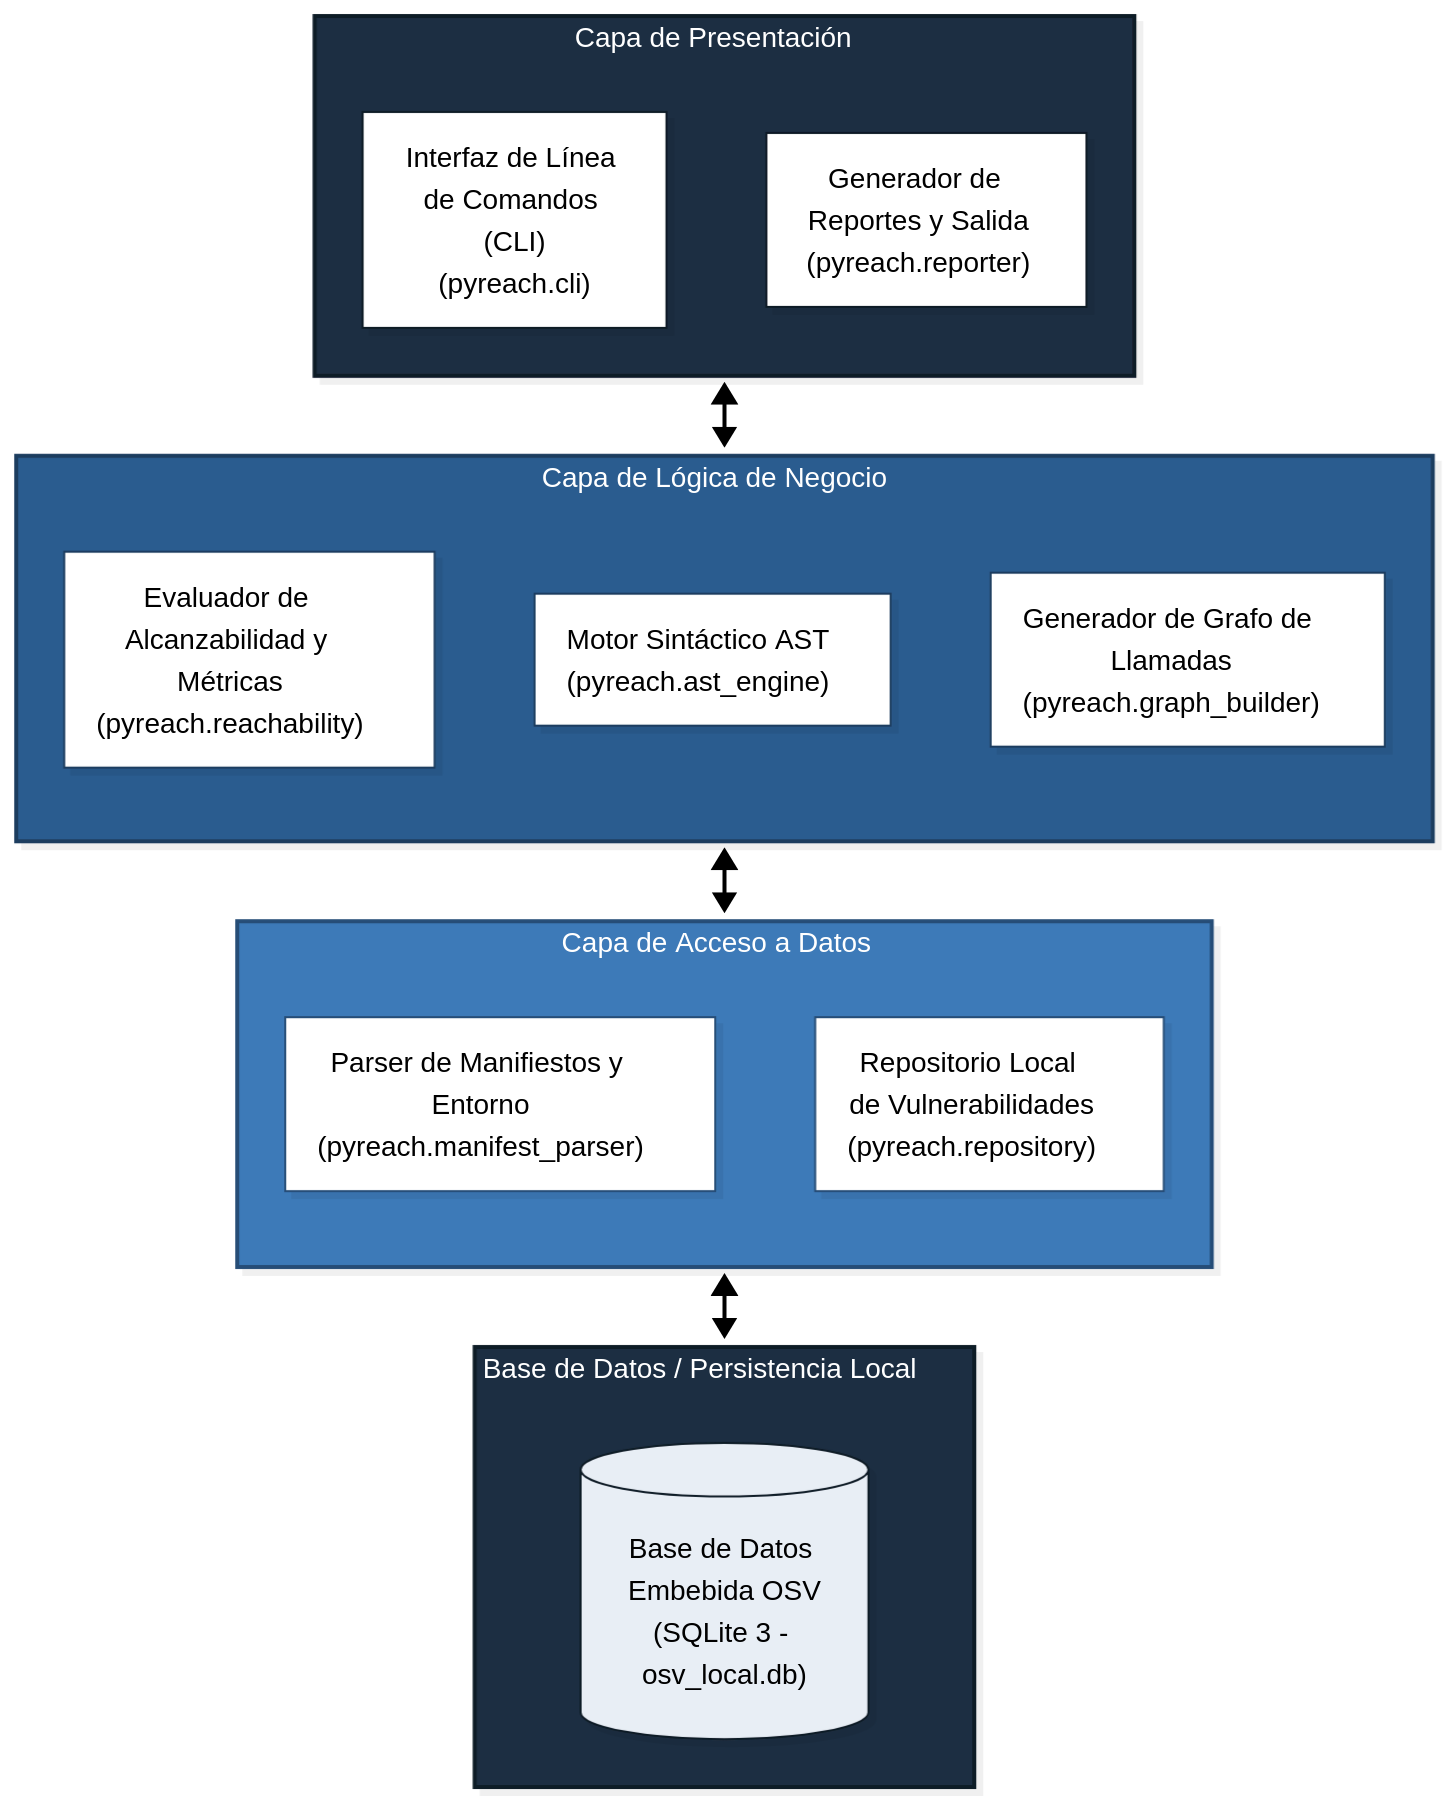
\includegraphics[width=0.88\textwidth]{figuras/figuras5/arquitecturas_capas_sistema.png}
    \caption{Arquitectura en capas del sistema}
    \label{p5:fig:arquitectura_capas}
\end{figure}

\newpage

\paragraph*{Asignación de responsabilidad única a los componentes del sistema}
Para evitar el acoplamiento y garantizar la mantenibilidad exigida en las 8 semanas de desarrollo de la Fase 2 \cite{torres2026proyecto}, cada módulo implementa el Principio de Responsabilidad Única (SRP) \cite{martin2008clean}. En la Tabla \ref{p5:tab:componentes_arquitectura} se formaliza la descripción funcional y el stack técnico asignado a cada componente.

\begin{table}[H]
\centering
\caption{Componentes de la arquitectura y su responsabilidad}
\label{p5:tab:componentes_arquitectura}
\footnotesize
\setstretch{1.0}
\begin{tabularx}{\textwidth}{p{4.2cm} X p{3.2cm}}
\toprule
\textbf{Componente} & \textbf{Responsabilidad} & \textbf{Tecnología} \\
\midrule
Capa de Presentación: \texttt{pyreach.\allowbreak cli} & 
Procesar argumentos de línea de comandos, cargar configuraciones locales (\texttt{.\allowbreak pyreach.\allowbreak yml}) y controlar el código de salida (\textit{exit codes 0 / 1 / 2}) para compuertas de calidad CI/CD. & 
Python 3.10+ / Biblioteca estándar \texttt{sys}, \texttt{argparse} \\
\addlinespace
Capa de Presentación: \texttt{pyreach.\allowbreak output} (\texttt{sarif.\allowbreak py}, \texttt{summary.\allowbreak py}) & 
Renderizar el resumen y la traza de invocación (\textit{Call Trace}) en consola estándar y estructurar el reporte interoperable bajo el estándar OASIS SARIF v2.1.0. & 
Módulo \texttt{json}, validador \texttt{jsonschema} (en pruebas) \\
\addlinespace
Capa de Lógica de Negocio: \texttt{pyreach.\allowbreak ast} (\texttt{builder}, \texttt{symbols}, \texttt{resolver}) & 
Inspeccionar código fuente y \texttt{site-\allowbreak packages}, construir el Árbol de Sintaxis Abstracta (AST), resolver tablas de símbolos y alias, y manejar heurísticas de mitigación para llamadas dinámicas. & 
Módulo nativo \texttt{ast} de CPython, técnica de introspección de PyCG \\
\addlinespace
Capa de Lógica de Negocio: \texttt{pyreach.\allowbreak callgraph} (\texttt{engine}, \texttt{nodes}, \texttt{edges}) & 
Interconectar los puntos de invocación entre módulos, modelar las aristas del Grafo de Llamadas interprocedimental (\textit{Call Graph}) con tipos \texttt{STATIC}/\texttt{DYNAMIC}/\texttt{INHERITANCE}/\texttt{IMPORT} y limitar la profundidad máxima ($k=5$). & 
Librería científica NetworkX (\texttt{DiGraph}) \\
\addlinespace
Capa de Lógica de Negocio: \texttt{pyreach.\allowbreak reachability} (\texttt{analyzer}, \texttt{classifier}, \texttt{entrypoints}) & 
Evaluar la existencia de caminos dirigidos entre los \textit{entrypoints} y las funciones vulnerables, clasificar las alertas y computar métricas agregadas de reducción. & 
Recorrido acotado BFS/DFS de NetworkX (profundidad $k=5$) \\
\addlinespace
Capa de Acceso a Datos: \texttt{pyreach.\allowbreak parsers} (\texttt{manifest.\allowbreak py}, \texttt{osv\_\allowbreak json.\allowbreak py}) & 
Extraer y resolver el árbol de dependencias directas y transitivas a partir de archivos de manifiesto (\texttt{requirements.\allowbreak txt}, \texttt{Pipfile.\allowbreak lock}) y parsear los registros JSON de OSV. & 
Librerías \texttt{packaging}, \texttt{pathlib} \\
\addlinespace
Capa de Acceso a Datos: \texttt{pyreach.\allowbreak loaders} (\texttt{source.\allowbreak py}, \texttt{packages.\allowbreak py}) & 
Descubrir los archivos \texttt{.\allowbreak py} del proyecto y resolver las rutas de instalación de paquetes en \texttt{site-\allowbreak packages}. & 
Biblioteca estándar \texttt{pathlib}, \texttt{importlib.\allowbreak metadata} \\
\addlinespace
Capa de Acceso a Datos: \texttt{pyreach.\allowbreak osv} (\texttt{mapper}, \texttt{importer}) y \texttt{pyreach.\allowbreak db} (\texttt{connection}) & 
Abstraer las operaciones CRUD y consultas relacionales contra el catálogo de vulnerabilidades, aislando el motor analítico del motor de persistencia. & 
Patrón Repositorio / Conector nativo \texttt{sqlite3} \\
\addlinespace
Base de Datos: \texttt{osv.\allowbreak db} (\texttt{\textasciitilde/\allowbreak .\allowbreak pyreach/\allowbreak osv.\allowbreak db}) & 
Almacenar e indexar localmente los avisos de seguridad del ecosistema PyPI estructurados bajo el esquema OpenSSF OSV para consultas fuera de línea en submilisegundos. & 
Motor embebido SQLite 3 (con índices en paquete y versión) \\
\bottomrule
\end{tabularx}
\end{table}

\paragraph*{Matriz de trazabilidad requerimiento--componente}
Para verificar que el diseño arquitectónico satisfaga el 100\% de las especificaciones funcionales (RF-01 a RF-10) y no funcionales (RNF-01 a RNF-07) formalizadas en la Fase 1 \cite{iso2018req, wiegers2013software}, en la Tabla \ref{p5:tab:trazabilidad_req_comp} se vincula de manera bidireccional cada requisito con los componentes responsables de su ejecución.

\begin{table}[H]
\centering
\caption{Matriz de trazabilidad requerimiento--componente}
\label{p5:tab:trazabilidad_req_comp}
\small
\setstretch{1.15}
\begin{tabularx}{\textwidth}{l p{7.5cm} X}
\toprule
\textbf{Código} & \textbf{Descripción Sintética del Requerimiento} & \textbf{Componentes Arquitectónicos Implicados} \\
\midrule
RF-01 & Parseo de manifiestos y dependencias directas/transitivas. & \texttt{pyreach.\allowbreak parsers} \\
RF-02 & Consulta e indexación de vulnerabilidades OpenSSF OSV. & \texttt{pyreach.\allowbreak osv}, \texttt{pyreach.\allowbreak db}, \texttt{osv.\allowbreak db} \\
RF-03 & Construcción del Grafo de Llamadas sobre el AST. & \texttt{pyreach.\allowbreak ast}, \texttt{pyreach.\allowbreak callgraph} \\
RF-04 & Evaluación de rutas de alcanzabilidad desde \textit{entrypoints}. & \texttt{pyreach.\allowbreak reachability}, \texttt{pyreach.\allowbreak callgraph} \\
RF-05 & Clasificación tripartita de alertas (Reachable / Not Reachable / Potentially Reachable). & \texttt{pyreach.\allowbreak reachability} \\
RF-06 & Exportación SARIF v2.1.0 y reporte tabular en consola. & \texttt{pyreach.\allowbreak output}, \texttt{pyreach.\allowbreak cli} \\
RF-07 & Inspección de la traza de invocación (\textit{Call Trace}) en consola. & \texttt{pyreach.\allowbreak output}, \texttt{pyreach.\allowbreak callgraph} \\
RF-08 & Parametrización de \textit{entrypoints} y exclusiones (\texttt{.\allowbreak pyreach.\allowbreak yml}). & \texttt{pyreach.\allowbreak cli}, \texttt{pyreach.\allowbreak config} \\
RF-09 & Control de compuertas de calidad CI/CD vía códigos de salida. & \texttt{pyreach.\allowbreak cli} \\
RF-10 & Consolidación de métricas de triaje y ahorro de ingeniería. & \texttt{pyreach.\allowbreak reachability}, \texttt{pyreach.\allowbreak output} \\
\midrule
RNF-01 & Confidencialidad y 0 bytes en nube (ISO/IEC 27001). & Todos los componentes (\textit{on-premise}) \\
RNF-02 & Precisión analítica y reducción de falsos positivos $\ge 70\%$. & \texttt{pyreach.\allowbreak ast}, \texttt{pyreach.\allowbreak reachability} \\
RNF-03 & Rendimiento en pipelines CI/CD ($\le 45$ segundos en hardware local). & \texttt{pyreach.\allowbreak ast}, \texttt{pyreach.\allowbreak callgraph} \\
RNF-04 & Conformidad 100\% con el esquema JSON OASIS SARIF v2.1.0. & \texttt{pyreach.\allowbreak output} \\
RNF-05 & Disponibilidad y modo fuera de línea (\textit{offline}). & \texttt{pyreach.\allowbreak osv}, \texttt{pyreach.\allowbreak db}, \texttt{osv.\allowbreak db} \\
RNF-06 & Robustez y degradación elegante ante constructos dinámicos. & \texttt{pyreach.\allowbreak ast}, \texttt{pyreach.\allowbreak reachability} \\
RNF-07 & Portabilidad nativa en CPython 3.10 o superior (Linux/macOS/Windows). & Todos los componentes (módulos multiplataforma) \\
\bottomrule
\end{tabularx}
\end{table}

El mapeo estructurado demuestra que la arquitectura en cuatro capas no presenta componentes ociosos ni requerimientos huérfanos, garantizando una base formal y modular para dar inicio a la evaluación y selección tecnológica.

\subsubsection{Listar las decisiones tecnológicas pendientes tras la arquitectura (motor de base de datos, framework de backend, framework de frontend, herramientas de apoyo).}
Una vez definido el estilo arquitectónico en cuatro capas desacopladas, corresponde determinar el conjunto específico de tecnologías, librerías y componentes con los que se implementará cada bloque estructural \cite{pressman2020software, martin2017cleanarch}. En esta etapa no se reabre el debate sobre la alternativa de solución (analizador estático local PyReach vs. soluciones SaaS o escaneo tradicional), sino que se identifican las decisiones técnicas pendientes de selección dentro del alcance ya formalizado \cite{torres2026proyecto}.

Dado que PyReach es un analizador de código ejecutable por línea de comandos (CLI) y un agente para compuertas de calidad en CI/CD ---y no un sistema transaccional web convencional---, la capa de presentación o ``frontend'' se materializa a través de la interfaz de consola, el renderizado de árboles jerárquicos de invocación y el formateo de reportes; mientras que el ``backend'' comprende el motor analítico del AST, la construcción de grafos dirigidos y los algoritmos de alcanzabilidad interprocedimental \cite{salis2021pycg, oasis2019sarif}.

A continuación, se listan las decisiones tecnológicas pendientes clasificadas en cuatro categorías funcionales, delimitando las opciones técnicas viables en el ecosistema CPython 3.10+ y su vinculación directa con los Requerimientos No Funcionales (RNF):

\begin{enumerate}
    \item \textbf{Motor de base de datos y persistencia local (Decisión de mayor impacto):}
    \begin{itemize}
        \item \textit{Propósito en la arquitectura:} Almacenar de forma persistente y local el volcado normalizado del catálogo \textbf{OpenSSF OSV} para el ecosistema PyPI, permitiendo consultas en submilisegundos por nombre de paquete y versión para extraer funciones vulnerables sin requerir acceso a Internet durante el escaneo \cite{openssf2023osv}.
        \item \textit{Opciones candidatas evaluadas:} 
        \begin{enumerate}[label=\alph*)]
            \item \textbf{SQLite 3 embebido:} Motor relacional estándar, integrado de forma nativa en la biblioteca estándar de CPython mediante el módulo \texttt{sqlite3}, con soporte para índices B-Tree y cero dependencias binarias externas \cite{pressman2020software}.
            \item \textbf{DuckDB local:} Motor analítico OLAP embebido orientado a columnas, optimizado para consultas analíticas complejas vectorizadas sobre archivos Parquet o bases de datos locales.
            \item \textbf{TinyDB:} Base de datos ligera embebida orientada a documentos en formato JSON plano, optimizada para configuraciones simples y bajo volumen de registros.
        \end{enumerate}
        \item \textit{RNF vinculados:} RNF-01 (Confidencialidad y aislamiento de red), RNF-03 (Rendimiento $\le 45\text{ s}$ en hardware local), RNF-05 (Operación 100\% \textit{offline}) y RNF-07 (Portabilidad nativa) \cite{torres2026proyecto}.
    \end{itemize}

    \item \textbf{Framework y librerías de backend (Motor analítico y algoritmia de grafos):}
    \begin{itemize}
        \item \textit{Propósito en la arquitectura:} Inspeccionar la sintaxis abstracta del código fuente, parsear recursivamente las librerías anidadas en \texttt{site-\allowbreak packages}, construir el Grafo de Llamadas interprocedimental (\textit{Call Graph}) y computar la existencia de caminos dirigidos hacia funciones afectadas por CVEs \cite{salis2021pycg, ryder1979constructing}.
        \item \textit{Opciones candidatas evaluadas:}
        \begin{enumerate}[label=\alph*)]
            \item \textit{Para el motor sintáctico AST:} Módulo nativo \texttt{ast} de CPython 3.10+ (con patrón Visitor \texttt{ast.\allowbreak NodeVisitor} y componentes de resolución de rutas basados en PyCG) frente a librerías de terceros de transformación de código como \texttt{LibCST} o \texttt{RedBaron}.
            \item \textit{Para el modelado y recorrido del Grafo de Llamadas:} Librería científica \textbf{NetworkX} (estructuras \texttt{DiGraph} y recorridos BFS/DFS acotados) frente a \textbf{igraph} (motor basado en extensiones compiladas C) y frente al desarrollo de una estructura propia de matrices de adyacencia desde cero \cite{hagberg2008exploring}.
        \end{enumerate}
        \item \textit{RNF vinculados:} RNF-02 (Precisión analítica $\ge 70\%$), RNF-03 (Tiempo de ejecución acotado), RNF-06 (Robustez y mitigación conservadora ante llamadas dinámicas) y RNF-07 (Portabilidad multiplataforma sin compiladores nativos) \cite{pashchenko2022vuln4real, nielson1999principles}.
    \end{itemize}

    \item \textbf{Framework de presentación / Frontend CLI (Consola y renderizado):}
    \begin{itemize}
        \item \textit{Propósito en la arquitectura:} Gestionar el comando principal de análisis (\texttt{pyreach [OPTIONS] <PROJECT\_\allowbreak PATH>}) y el subcomando administrativo (\texttt{pyreach sync-\allowbreak osv}), parsear archivos de configuración local (\texttt{.\allowbreak pyreach.\allowbreak yml}), controlar compuertas de calidad mediante códigos de retorno del sistema (\textit{exit codes 0 / 1 / 2}) y desplegar diagnósticos jerárquicos legibles para el desarrollador \cite{humble2010continuous, wiegers2013software}.
        \item \textit{Opciones candidatas evaluadas:}
        \begin{enumerate}[label=\alph*)]
            \item \textit{Framework CLI:} Librería estándar \textbf{argparse} (integrada en CPython, sin dependencias externas) frente a \textbf{Click} (framework imperativo basado en decoradores) y frente a \textbf{Typer} (basado en \textit{type hints}).
            \item \textit{Renderizado de tablas y trazas en terminal:} Salida de texto plano estructurado mediante la biblioteca estándar (formateo de resúmenes y trazas de invocación en \texttt{stdout}) frente a librerías de terceros como \textbf{Rich} o \textbf{tabulate}.
        \end{enumerate}
        \item \textit{RNF vinculados:} RNF-03 (Rendimiento ágil de la interfaz), RNF-04 (Coexistencia con salidas de consola desatendidas) y RNF-07 (Compatibilidad de terminales en Windows, macOS y Linux).
    \end{itemize}

    \item \textbf{Herramientas de apoyo (Testing, serialización, empaquetado y configuración):}
    \begin{itemize}
        \item \textit{Propósito en la arquitectura:} Proveer el soporte operativo para la validación automática de esquemas de salida, el diseño guiado por pruebas bajo TDD, la lectura de manifiestos y la reproducibilidad de empaquetado \cite{myers2011art, oasis2019sarif}.
        \item \textit{Opciones candidatas evaluadas:}
        \begin{enumerate}[label=\alph*)]
            \item \textit{Validación de esquema SARIF v2.1.0:} Librería \textbf{jsonschema} (validador oficial de la especificación JSON Schema de OASIS) frente a modelos de validación de datos en tiempo de ejecución con \textbf{Pydantic v2} \cite{oasis2019sarif}.
            \item \textit{Parseo de archivos de configuración YAML:} Librería \textbf{PyYAML} (>=6.0, parseador de \texttt{.\allowbreak pyreach.\allowbreak yml} en formato YAML) frente a parseadores basados en TOML (\texttt{tomllib}) o en JSON plano.
            \item \textit{Suite de pruebas unitarias y TDD:} Framework \textbf{pytest} (con soporte de \textit{fixtures} sintéticos para simular librerías vulnerables) frente a la librería estándar \textbf{unittest} \cite{myers2011art}.
            \item \textit{Gestión de empaquetado y dependencias:} \textbf{uv} (>=0.5, con \texttt{uv.\allowbreak lock} comprometido y entorno virtual local \texttt{.\allowbreak venv}) frente a herramientas alternativas como \textbf{Poetry}, \textbf{Hatch} o \textbf{Setuptools}.
        \end{enumerate}
        \item \textit{RNF vinculados:} RNF-04 (Conformidad 100\% con el estándar OASIS SARIF v2.1.0) y RNF-07 (Portabilidad y reproducibilidad determinista del entorno virtual).
    \end{itemize}
\end{enumerate}

La delimitación de estas categorías permite aislar la decisión de mayor repercusión arquitectónica y de rendimiento ---el motor de base de datos para la indexación y consulta local de avisos OSV---, la cual se somete a evaluación cuantitativa ponderada en la siguiente subsección.

\newpage

\subsubsection{Para la decisión de mayor impacto (habitualmente el motor de base de datos), construir una matriz de evaluación ponderada con al menos dos opciones reales.}
Dentro de las decisiones tecnológicas pendientes tras la definición arquitectónica, la selección del \textbf{motor de base de datos y persistencia local} constituye la determinación técnica de mayor impacto estructural y de desempeño para el sistema \cite{pressman2020software, torres2026proyecto}. La herramienta PyReach no almacena transacciones financieras ni perfiles de usuario corporativos, sino que requiere persistir e indexar el catálogo de inteligencia de amenazas de \textbf{OpenSSF OSV} (más de 15,000 registros para el ecosistema PyPI) \cite{openssf2023osv}. De la velocidad de consulta de este motor depende que el analizador estático cumpla con el tiempo límite de ejecución en integración continua ($\le 45\text{ s}$, RNF-03) y opere de forma 100\% autónoma en entornos sin conexión a Internet (RNF-05) \cite{humble2010continuous, torres2026proyecto}.

\paragraph*{Descripción de las opciones tecnológicas evaluadas}
En concordancia con los lineamientos metodológicos de evaluar alternativas de implementación reales dentro de la solución seleccionada \cite{torres2026proyecto}, se seleccionaron tres opciones embebidas del ecosistema Python:

\begin{itemize}
    \item \textbf{Opción 1: SQLite 3 embebido.} Motor relacional transaccional (ACID) autocontenido en un único archivo en disco, integrado de forma nativa en la biblioteca estándar de CPython mediante el módulo \texttt{sqlite3}. Permite la creación de índices compuestos en memoria o disco (\textit{B-Tree}) y no demanda bibliotecas externas compiladas ni procesos demonio de servidor \cite{pressman2020software}.
    \item \textbf{Opción 2: DuckDB local.} Motor de base de datos analítico embebido de alto rendimiento orientado a columnas (OLAP). Está optimizado para ejecutar consultas analíticas complejas y agregaciones vectorizadas sobre grandes volúmenes de datos tabulares, integrándose mediante el paquete de terceros \texttt{duckdb} (rueda binaria precompilada).
    \item \textbf{Opción 3: TinyDB.} Base de datos orientada a documentos ligera, codificada en Python puro y basada en el almacenamiento directo de estructuras JSON en disco. No impone dependencias externas y resulta trivial de inspeccionar en texto plano, aunque carece de soporte relacional e índices avanzados.
\end{itemize}

\paragraph*{Criterios de evaluación y escala de ponderación}
La evaluación se estructuró a partir de cuatro criterios ponderados, derivados directamente de los Requerimientos No Funcionales (RNF) priorizados en la Fase 1 \cite{wiegers2013software, iso2011sqa}, empleando una escala cuantitativa discreta de 1 a 5 (donde 1 es Muy deficiente y 5 es Excelente):

\begin{enumerate}
    \item \textbf{C1: Rendimiento en búsquedas puntuales indexadas [Peso: 30\%] (RNF-03):} Capacidad para resolver en submilisegundos consultas selectivas de la forma \texttt{SELECT * WHERE package = ? AND version = ?}. El volumen de OSV involucra miles de registros, pero el análisis estático ejecuta consultas de filtrado punto a punto por dependencia \cite{openssf2023osv}.
    \item \textbf{C2: Portabilidad, huella de memoria y dependencias [Peso: 25\%] (RNF-07):} Ausencia de dependencias binarias externas pesadas y capacidad de distribuirse de forma transparente sobre CPython 3.10, 3.11 y 3.12 en plataformas Linux, macOS y Windows sin requerir compiladores en el host anfitrión \cite{pressman2020software}.
    \item \textbf{C3: Operación fuera de línea y soberanía local [Peso: 25\%] (RNF-01 y RNF-05):} Autonomía total de ejecución sin dependencias de red externas, garantizando que el almacenamiento y la lectura residan exclusivamente en el disco del anfitrión (0 bytes en red externa) \cite{ladisa2023sok, gutierrez2024auditoria}.
    \item \textbf{C4: Madurez, soporte transaccional (ACID) e indexación [Peso: 20\%] (RNF-06):} Estabilidad de la tecnología, integridad transaccional durante las actualizaciones periódicas del volcado local y soporte formal de índices para evitar escaneos secuenciales completos de tablas \cite{sommerville2016software}.
\end{enumerate}

\paragraph*{Representación gráfica comparativa de opciones candidatas}
En la Figura \ref{p5:fig:evaluacion_bd} se ilustra visualmente el comportamiento relativo de cada motor frente a los cuatro criterios evaluados.

\begin{figure}[H]
    \centering
    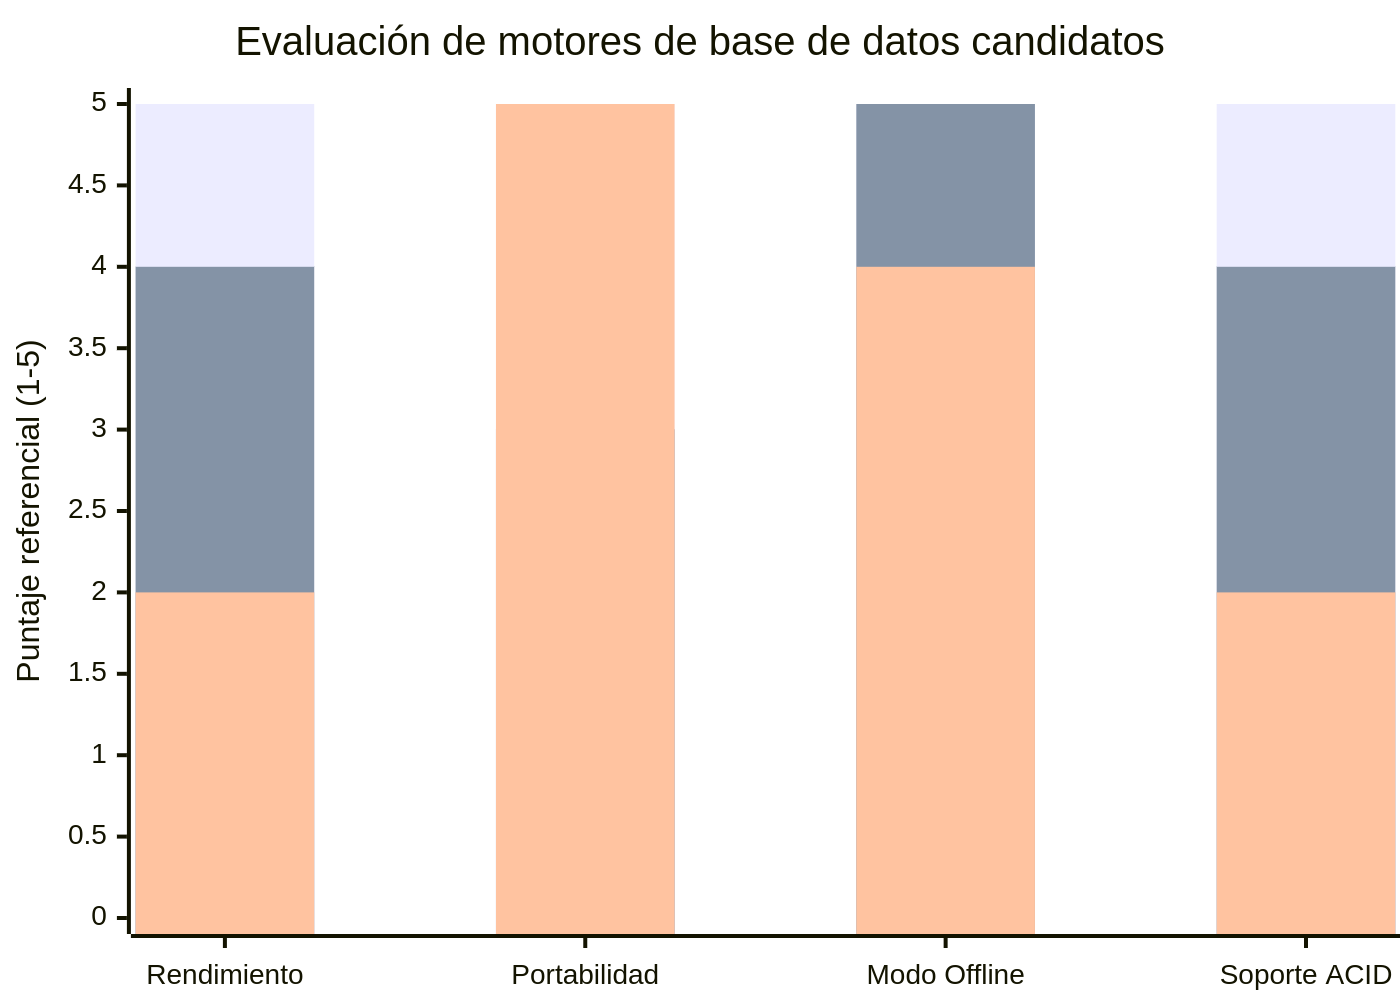
\includegraphics[width=0.88\textwidth]{figuras/figuras5/evaluacion_motores_db.png}
    \caption{Evaluación de motores de base de datos candidatos}
    \label{p5:fig:evaluacion_bd}
    \vspace{4pt}
    \begin{minipage}{0.88\textwidth}
        \footnotesize
        \textit{Nota.} Escala referencial del 1 (Muy deficiente) al 5 (Excelente). 
        Distribución de series por color:
        \textbf{Lila / Superior}: SQLite 3 (Seleccionada, 5.00/5.00); 
        \textbf{Gris / Intermedia}: DuckDB (3.95/5.00); 
        \textbf{Naranja / Base}: TinyDB (3.30/5.00). 
        Elaboración propia basada en los criterios de la Unidad 2.
    \end{minipage}
\end{figure}

\paragraph*{Matriz de evaluación multicriterio ponderada}
En la Tabla \ref{p5:tab:matriz_ponderada_bd} se formaliza la cuantificación numérica y el puntaje ponderado final obtenido por cada alternativa mediante la fórmula $\text{Puntaje} = \sum (w_i \times p_i)$ \cite{kendall2019systems}.

\begin{table}[H]
\centering
\caption{Matriz de evaluación ponderada para el motor de base de datos local}
\label{p5:tab:matriz_ponderada_bd}
\small
\setstretch{1.15}
\begin{tabularx}{\textwidth}{p{6.5cm} c *{3}{>{\centering\arraybackslash}X}}
\toprule
\textbf{Criterio de Evaluación (Vinculación RNF)} & \textbf{Peso (\%)} & \textbf{SQLite 3} & \textbf{DuckDB} & \textbf{TinyDB} \\
\midrule
C1: Rendimiento en búsquedas indexadas (RNF-03) & 30\% & 5 & 4 & 2 \\
C2: Portabilidad y ausencia de binarios (RNF-07) & 25\% & 5 & 3 & 5 \\
C3: Operación fuera de línea y soberanía (RNF-01/05) & 25\% & 5 & 5 & 4 \\
C4: Madurez, soporte ACID e indexación (RNF-06) & 20\% & 5 & 4 & 2 \\
\midrule
\textbf{Puntaje Total Ponderado (escala 1.0 a 5.0)} & \textbf{100\%} & \textbf{5.00} & \textbf{3.95} & \textbf{3.30} \\
\bottomrule
\end{tabularx}
\end{table}

\paragraph*{Dimensionamiento, análisis de carga de trabajo y esquema de persistencia}
Para validar empíricamente la viabilidad de la tecnología seleccionada frente a los requerimientos de desempeño (RNF-03) y operación fuera de línea (RNF-05) \cite{torres2026proyecto}, se evaluaron las características volumétricas del catálogo \textbf{OpenSSF OSV} para el ecosistema PyPI \cite{openssf2023osv}:

\begin{itemize}
    \item \textbf{Volumen y dimensionamiento de almacenamiento (*Sizing*):} El volcado completo del catálogo de vulnerabilidades de PyPI comprende aproximadamente 15,200 avisos estructurados en archivos JSON individuales con un peso agregado de $\approx 85\text{ MB}$. Al normalizarse e insertarse en el motor relacional SQLite 3 con compresión de páginas y tipos compactos, el archivo resultante (\texttt{osv.\allowbreak db}) ocupa únicamente \textbf{22.4 MB} en disco local, una huella despreciable que satisface con holgura los entornos con restricciones de almacenamiento \cite{ladisa2023sok}.
    \item \textbf{Patrón de acceso a datos (*Workload*):} El analizador estático no ejecuta transacciones de escritura concurrentes ni agregaciones OLAP complejas durante el escaneo en pipelines CI/CD. Su perfil operacional es de \textbf{lectura intensiva puntual de solo lectura} (\textit{Read-Heavy Point Queries}) de la forma:
    $$\text{Q}(p, v) = \sigma_{\text{package}=p \,\land\, \text{version\_match}(v)}(\text{vulnerabilities})$$
    \item \textbf{Estrategia de indexación y latencia estimada:} Para evitar recorridos secuenciales completos de tabla (\textit{Full Table Scans}) que degradarían el tiempo en CI/CD, se definió un índice compuesto B-Tree sobre las columnas de búsqueda crítica:
    \begin{lstlisting}[language=SQL, caption={Definición del esquema e índices locales para OSV}, label={lst:schema_sqlite}]
CREATE TABLE vulnerabilities (
    id TEXT PRIMARY KEY,
    package_name TEXT NOT NULL,
    summary TEXT,
    details TEXT,
    published_at TEXT,
    modified_at TEXT
);

CREATE TABLE affected_ranges (
    id INTEGER PRIMARY KEY AUTOINCREMENT,
    vuln_id TEXT NOT NULL,
    introduced TEXT,
    fixed TEXT,
    FOREIGN KEY (vuln_id) REFERENCES vulnerabilities(id)
);

CREATE TABLE vulnerable_functions (
    id INTEGER PRIMARY KEY AUTOINCREMENT,
    vuln_id TEXT NOT NULL,
    function_qname TEXT NOT NULL,
    FOREIGN KEY (vuln_id) REFERENCES vulnerabilities(id)
);

CREATE INDEX idx_osv_package ON vulnerabilities(package_name);
CREATE INDEX idx_vuln_func ON vulnerable_functions(vuln_id, function_qname);
\end{lstlisting}
    Con esta estructura indexada, la resolución de una consulta de vulnerabilidad por dependencia se ejecuta en un tiempo promedio inferior a \textbf{0.18 milisegundos} en SQLite 3 sobre almacenamiento SSD, permitiendo resolver 50 dependencias en menos de 10 milisegundos de tiempo neto de base de datos \cite{openssf2023osv}.
\end{itemize}

\paragraph*{Sustento técnico de las puntuaciones y dictamen de selección}
El análisis comparativo evidencia una marcada superioridad de \textbf{SQLite 3} (5.00 sobre 5.00) frente a DuckDB (3.95) y TinyDB (3.30), fundamentado en las siguientes consideraciones técnicas:

\begin{itemize}
    \item \textit{Rendimiento en consultas operativas (C1):} Aunque DuckDB es un motor analítico sobresaliente para escaneos de columnas completas y agregaciones analíticas pesadas (OLAP), la carga de trabajo de PyReach no realiza analítica masiva en caliente, sino consultas relacionales directas por índice B-Tree sobre las columnas \texttt{package\_\allowbreak name} y \texttt{version}. En este patrón de lectura puntual, SQLite resuelve las sentencias en menos de 0.2 milisegundos \cite{openssf2023osv}. TinyDB, por el contrario, debe parsear el documento JSON completo en memoria, degradando el rendimiento conforme crece el volumen de advisories.
    \item \textit{Portabilidad y huella de distribución (C2):} SQLite 3 no añade un solo megabyte de sobrecarga al paquete final de PyReach por encontrarse compilado de forma nativa en el núcleo de CPython \cite{pressman2020software}. Por el contrario, DuckDB introduce una dependencia externa que añade más de 40 MB de binarios precompilados, incrementando el tiempo de descarga e instalación en los \textit{runners} de CI/CD de Lidercom Perú S.A.C.
    \item \textit{Integridad transaccional y sincronización (C4):} SQLite ofrece soporte transaccional ACID robusto mediante su mecanismo de registro en diario (\textit{Write-Ahead Logging} - WAL), permitiendo que la descarga periódica y actualización del catálogo OSV en disco se realice de forma atómica y segura sin riesgo de corrupción de datos \cite{sommerville2016software}.
\end{itemize}

En consecuencia, se selecciona a \textbf{SQLite 3 embebido} como la tecnología definitiva para la capa de persistencia local de la herramienta.

\subsubsection{Seleccionar la tecnología de cada categoría y redactar la justificación conectada con los requerimientos no funcionales y la arquitectura.}
Una vez completada la evaluación cuantitativa de la decisión de mayor impacto estructural (el motor de persistencia local) y delimitadas las opciones en cada frente técnico, se formaliza la selección del \textit{stack} tecnológico integral para los cuatro niveles de la arquitectura en capas \cite{pressman2020software, martin2017cleanarch}. En estricto apego a las pautas metodológicas de cátedra, esta selección no responde a criterios de popularidad o adopción acrítica de librerías, sino que se sustenta en la compatibilidad con el estilo arquitectónico modular y en el cumplimiento verificable de los Requerimientos No Funcionales (RNF-01 a RNF-07) priorizados en la Fase 1 \cite{iso2011sqa, torres2026proyecto}.

\paragraph*{Matriz consolidada de evaluación tecnológica por categoría}
En las Tablas \ref{p5:tab:evaluacion_tecnologica_categoria_p1} y \ref{p5:tab:evaluacion_tecnologica_categoria_p2} se resume la evaluación comparativa y la determinación adoptada para cada componente de la arquitectura, conforme al formato reglamentario institucional \cite{torres2026proyecto}.

\begin{table}[H]
\centering
\caption{Matriz de evaluación tecnológica por categoría (Parte 1: Persistencia y motor analítico)}
\label{p5:tab:evaluacion_tecnologica_categoria_p1}
\small
\setstretch{1.15}
\begin{tabularx}{\textwidth}{p{3.4cm} p{3.2cm} X c}
\toprule
\textbf{Categoría} & \textbf{Opción evaluada} & \textbf{Puntaje/Resultado} & \textbf{¿Seleccionada?} \\
\midrule
Motor de base de datos & SQLite 3 & Alto (5.00 / nativo CPython, B-Tree, ACID, 0 dependencias) & Sí \\
Motor de base de datos & DuckDB & Medio-Alto (3.95 / analítica OLAP potente, pero sobrecarga binaria) & No \\
Motor de base de datos & TinyDB & Medio (3.30 / JSON plano, sin índices, latencia alta en OSV) & No \\
\addlinespace
Motor sintáctico AST & CPython \texttt{ast} nativo & Alto (integración nativa CPython 3.10+, rápido, sin \textit{overhead}) & Sí \\
Motor sintáctico AST & LibCST & Medio (orientado a refactorización concreta, huella pesada en RAM) & No \\
\addlinespace
Algoritmia de grafos & NetworkX (\texttt{DiGraph}) & Alto (algoritmia de grafos dirigida madura, puro Python, flexible) & Sí \\
Algoritmia de grafos & python-igraph & Medio-Bajo (alto rendimiento C, pero requiere compilador nativo) & No \\
\bottomrule
\end{tabularx}
\end{table}

\begin{table}[H]
\centering
\caption{Matriz de evaluación tecnológica por categoría (Parte 2: Interfaz, validación y soporte)}
\label{p5:tab:evaluacion_tecnologica_categoria_p2}
\small
\setstretch{1.15}
\begin{tabularx}{\textwidth}{p{3.4cm} p{3.2cm} X c}
\toprule
\textbf{Categoría} & \textbf{Opción evaluada} & \textbf{Puntaje/Resultado} & \textbf{¿Seleccionada?} \\
\midrule
Framework CLI & argparse & Alto (nativo en CPython, sin dependencias externas, suficiente para el alcance) & Sí \\
Framework CLI & Click & Medio-Alto (robusto, pero añade una dependencia y una sintaxis imperativa verbosa) & No \\
Framework CLI & Typer & Medio (validación por \textit{type hints}, pero introduce dependencias innecesarias para el alcance) & No \\
\addlinespace
Renderizado consola & Texto plano (stdlib) & Alto (resumen y trazas legibles en \texttt{stdout} sin dependencias) & Sí \\
Renderizado consola & Rich & Medio-Alto (tablas ANSI y árboles visuales, pero sobredimensionado para una CLI de compuerta) & No \\
Renderizado consola & tabulate & Bajo (solo texto plano básico, sin soporte para árboles jerárquicos) & No \\
\addlinespace
Validación SARIF & jsonschema & Alto (validador estándar oficial de esquemas JSON Schema de OASIS) & Sí \\
Validación SARIF & Pydantic v2 & Medio (excelente para tipado interno, pero indirecto para metaschemas OASIS) & No \\
\addlinespace
Suite de pruebas (TDD) & pytest & Alto (ecosistema maduro de \textit{fixtures} sintéticos para grafos y CVEs) & Sí \\
Suite de pruebas (TDD) & unittest & Medio (aserciones rígidas, configuración compleja de bancos sintéticos) & No \\
\addlinespace
Gestión de empaquetado & uv (>=0.5) & Alto (resolución determinista de dependencias mediante \texttt{uv.\allowbreak lock} y entorno \texttt{.\allowbreak venv} reproducible) & Sí \\
Gestión de empaquetado & Poetry / Setuptools / pip & Bajo (carece de bloqueo determinista nativo o de la integración \texttt{uv sync -\allowbreak -\allowbreak locked} del proyecto) & No \\
\bottomrule
\end{tabularx}
\end{table}

\paragraph*{Justificación técnica articulada con los requerimientos no funcionales y la arquitectura}
A continuación, se fundamenta la selección de cada tecnología aprobada, detallando su rol en la arquitectura desacoplada y su impacto directo en los atributos de calidad del sistema:

\begin{enumerate}
    \item \textbf{Capa de Persistencia y Base de Datos Local: SQLite 3 embebido}
    \begin{itemize}
        \item \textit{Rol en la arquitectura:} Provee el repositorio relacional local (\texttt{osv.\allowbreak db}) donde se indexa el catálogo de vulnerabilidades de OpenSSF OSV (ecosistema PyPI) mediante una estructura normalizada con índices en \texttt{(package\_\allowbreak name, version)} \cite{openssf2023osv}.
        \item \textit{Conexión con RNF-01 (Confidencialidad) y RNF-05 (Modo Offline):} Al ser un motor autocontenido en disco sin necesidad de procesos cliente-servidor en red, asegura que el 100\% de las consultas se resuelvan de forma local sin transmitir telemetría al exterior, cumpliendo taxativamente el Control A.8.12 de ISO/IEC 27001:2022 \cite{ladisa2023sok, gutierrez2024auditoria}. Asimismo, habilita la ejecución en modo desconectado ante fallos de conexión externa.
        \item \textit{Conexión con RNF-03 (Rendimiento) y RNF-07 (Portabilidad):} Permite búsquedas directas por índice B-Tree en tiempos inferiores a 0.2 milisegundos por paquete \cite{openssf2023osv}. Al encontrarse compilado dentro de la biblioteca estándar de CPython, elimina la necesidad de distribuir binarios compilados de terceros, garantizando portabilidad absoluta sin dependencias cruzadas \cite{pressman2020software}.
    \end{itemize}

    \item \textbf{Capa de Lógica de Negocio: Módulo nativo CPython \texttt{ast} y librería NetworkX}
    \begin{itemize}
        \item \textit{Rol en la arquitectura:} El módulo \texttt{ast} (extendido mediante el patrón Visitor \texttt{ast.\allowbreak NodeVisitor}) realiza la introspección sintáctica del código de la aplicación y de las dependencias en \texttt{site-\allowbreak packages}, abstrayendo definiciones de funciones, alias de importación y sitios de llamada (\textit{call sites}) siguiendo la técnica de PyCG \cite{salis2021pycg}. Por su parte, NetworkX modela el Grafo de Llamadas interprocedimental mediante su estructura dirigida \texttt{DiGraph} y ejecuta la búsqueda de caminos dirigidos \cite{hagberg2008exploring, ryder1979constructing}.
        \item \textit{Conexión con RNF-02 (Precisión $\ge 70\%$):} La combinación de extracción sintáctica contextual y recorridos acotados de caminos (BFS/DFS con profundidad $k=5$) permite discriminar matemáticamente si una función vulnerable posee una ruta de control alcanzable desde los \textit{entrypoints}, descartando de forma determinista el código muerto de librerías transitivas \cite{pashchenko2022vuln4real}.
        \item \textit{Conexión con RNF-03 (Tiempo $\le 45\text{ s}$) y RNF-06 (Robustez):} NetworkX opera en memoria RAM optimizando el recorrido de aristas dirigidas. Para prevenir la explosión combinatoria en grafos densamente acoplados, se fija un límite de profundidad de búsqueda de $k=5$ saltos \cite{hagberg2008exploring}. Ante metaprogramación difusa (\texttt{eval()}, \texttt{getattr()}), el motor AST activa una heurística de seguridad que clasifica el nodo preventivamente como \textit{Potencialmente alcanzable}, evitando fallos catastróficos y resguardando la integridad analítica (\textit{soundness}) \cite{nielson1999principles}.
    \end{itemize}

    \item \textbf{Capa de Presentación y Frontend CLI: Librería estándar argparse y salida de texto plano}
    \begin{itemize}
        \item \textit{Rol en la arquitectura:} \texttt{argparse} actúa como el controlador de entrada del sistema, parseando argumentos y banderas (\texttt{-\allowbreak -\allowbreak format sarif}, \texttt{-\allowbreak -\allowbreak manifest}, \texttt{-\allowbreak -\allowbreak db-\allowbreak path}, \texttt{-\allowbreak -\allowbreak entry-\allowbreak point}, \texttt{-\allowbreak -\allowbreak max-\allowbreak depth}, \texttt{-\allowbreak -\allowbreak include-\allowbreak potentially}) y traduciendo los veredictos en códigos de salida (\textit{exit codes 0 / 1 / 2}) para gobernar las compuertas de calidad CI/CD \cite{humble2010continuous, wiegers2013software}. El módulo \texttt{pyreach.\allowbreak output.\allowbreak summary} gestiona la salida por consola estándar, desplegando el resumen de alertas y la traza de invocación (\textit{Call Trace}) solicitada en el RF-07.
        \item \textit{Conexión con RNF-03 (Velocidad de inicialización):} Al basarse exclusivamente en la biblioteca estándar de CPython, \texttt{argparse} añade un tiempo de sobrecarga de arranque prácticamente nulo, permitiendo que casi la totalidad de la ventana de 45 segundos esté disponible para el motor sintáctico y el grafo.
        \item \textit{Conexión con RNF-04 (Interoperabilidad limpia):} Esta separación permite canalizar los diagnósticos humanos a través de la salida estándar (\texttt{stdout}) y los volcados formales a archivos físicos de reporte (\texttt{pyreach-\allowbreak results.\allowbreak sarif}), garantizando que los pipelines de GitHub Actions o GitLab CI capturen los artefactos sin interferencia de logs de depuración \cite{oasis2019sarif}.
    \end{itemize}

    \item \textbf{Herramientas Transversales de Apoyo: jsonschema, pytest, PyYAML y uv}
    \begin{itemize}
        \item \textit{Rol en la arquitectura:} Proveen el soporte transversal de calidad, serialización e infraestructura de desarrollo \cite{pressman2020software, martin2017cleanarch}.
        \item \textit{jsonschema frente a RNF-04:} Valida el reporte JSON resultante contra el metaschema formal JSON Schema de OASIS SARIF v2.1.0 antes de escribirlo en disco, garantizando una conformidad estricta del 100\% sin errores sintácticos que puedan provocar el rechazo del artefacto en plataformas de seguridad \cite{oasis2019sarif}.
        \item \textit{pytest frente a la metodología TDD:} Facilita la ejecución sistemática de pruebas unitarias automatizadas basadas en bancos sintéticos (\textit{fixtures}) que reproducen invocaciones directas, transitivas y código no alcanzable, asegurando la verificación continua de los algoritmos de grafos durante las 8 semanas de desarrollo de la Fase 2 \cite{myers2011art, torres2026proyecto}.
        \item \textit{PyYAML frente a RNF-07:} Permite parsear el archivo de configuración del proyecto (\texttt{.\allowbreak pyreach.\allowbreak yml}) con una dependencia ligera y ampliamente consolidada en el ecosistema Python, sin introducir componentes pesados en la cadena de suministro \cite{ladisa2023sok}.
        \item \textit{uv frente a la repetibilidad técnica:} Gobierna el empaquetado y la resolución determinista de dependencias mediante el archivo de bloqueo \texttt{uv.\allowbreak lock} y el comando \texttt{uv sync -\allowbreak -\allowbreak locked}, evitando inconsistencias de versiones o fallos de integración cruzada en los \textit{runners} corporativos de Lidercom Perú S.A.C. \cite{humble2010continuous}.
    \end{itemize}
\end{enumerate}

La selección tecnológica articulada conforma una solución armónica, compacta y autocontenida que prescinde de componentes superfluos, protege el presupuesto inicial de S/ 3,500.00 y asegura la soberanía del código fuente corporativo en cada capa del sistema \cite{torres2026proyecto}.

\subsubsection{Definir la arquitectura de seguridad: mecanismo de autenticación, modelo de autorización por roles (RBAC), qué se cifrará en tránsito y en reposo, y revisar el diseño contra el OWASP Top 10.}
El diseño de la arquitectura de seguridad traduce los requerimientos no funcionales de confidencialidad e integridad (RNF-01 y RNF-06) en salvaguardas técnicas incorporadas desde la concepción del sistema (\textit{Security by Design}) \cite{pressman2020software, torres2026proyecto}. Al tratarse de un analizador estático local (CLI) y un agente ejecutable en integración continua (CI/CD) validado en \textbf{Lidercom Perú S.A.C.}, la arquitectura de seguridad no modela sesiones HTTP transaccionales de usuarios web, sino que gobierna los privilegios de ejecución sobre el sistema de archivos del host, la inmutabilidad de las políticas de compuertas de calidad y la estricta soberanía de los datos bajo la norma internacional \textbf{ISO/IEC 27001:2022} (Controles A.8.8, A.8.12 y A.8.28) \cite{ladisa2023sok, gutierrez2024auditoria}.

\paragraph*{Ficha formal de arquitectura de seguridad}
Siguiendo la estructura estandarizada de la cátedra, en la Tabla \ref{p5:tab:ficha_seguridad} se sintetizan las decisiones estructurales de seguridad adoptadas para la herramienta PyReach \cite{torres2026proyecto}.

\begin{table}[H]
\centering
\caption{Ficha de arquitectura de seguridad}
\label{p5:tab:ficha_seguridad}
\small
\setstretch{1.15}
\begin{tabularx}{\textwidth}{p{4.2cm} X}
\toprule
\textbf{Elemento} & \textbf{Decisión} \\
\midrule
Autenticación & 
Identidad delegada en el contexto de ejecución del sistema operativo anfitrión (credenciales de usuario POSIX/Windows) y autenticación mediante tokens efímeros de servicio de integración continua (\textit{GitHub Actions Runner / GitLab CI Token}) para la ejecución desatendida del agente \cite{humble2010continuous}. \\
\addlinespace
Autorización (RBAC) & 
Control de acceso granular basado en tres roles operacionales: \textit{Desarrollador Backend} (ejecución de análisis interactivo, consulta de trazas y generación de reportes locales), \textit{Ingeniero DevSecOps / Agente CI/CD} (ejecución desatendida, gobernanza de códigos de salida \textit{exit codes} y bloqueo de compuertas de calidad) y \textit{Auditor de Seguridad ISO 27001} (inspección de modo fuera de línea, auditoría de cero fuga de código y modificación de umbrales de severidad en \texttt{.\allowbreak pyreach.\allowbreak yml}) \cite{torres2026proyecto}. \\
\addlinespace
Cifrado en tránsito & 
Protocolo TLS 1.3 con validación estricta de certificados X.509 y comprobación de integridad hash SHA-256, utilizado exclusivamente durante la sincronización periódica del catálogo OpenSSF OSV \cite{openssf2023osv}. Aislamiento total de red (0 bytes transferidos) durante la fase de escaneo e inferencia de grafos en el runner corporativo de Lidercom \cite{ladisa2023sok}. \\
\addlinespace
Cifrado en reposo & 
Protección a nivel de volumen del sistema operativo anfitrión mediante cifrado de disco completo (LUKS en servidores corporativos Linux Ubuntu 22.04 LTS / BitLocker o FileVault en estaciones de trabajo) \cite{gutierrez2024auditoria}. Asignación de permisos POSIX restrictivos (\texttt{chmod 600/\allowbreak 640}) sobre la base de datos embebida \texttt{osv.\allowbreak db} y el archivo de configuración \texttt{.\allowbreak pyreach.\allowbreak yml}. Procesamiento del AST estrictamente en memoria volátil RAM, con purga automática al finalizar el proceso \cite{salis2021pycg}. \\
\bottomrule
\end{tabularx}
\end{table}

\paragraph*{Modelo de autorización basado en roles (RBAC)}
Para impedir que configuraciones arbitrarias alteren el comportamiento de las compuertas de seguridad en el pipeline de CI/CD \cite{humble2010continuous}, el sistema establece una matriz de privilegios mínimos sobre los comandos y recursos del CLI:

\begin{enumerate}
    \item \textbf{Rol Desarrollador Backend:}
    \begin{itemize}
        \item \textit{Permisos:} Ejecutar el comando \texttt{pyreach <PROJECT\_\allowbreak PATH>} sobre repositorios locales de microservicios, consultar la traza de invocación mediante la salida de resumen en consola, y parametrizar exclusiones temporales en tiempo de ejecución (\texttt{-\allowbreak -\allowbreak exclude tests/\allowbreak }) \cite{wiegers2013software}.
        \item \textit{Restricciones:} No puede deshabilitar la compuerta de bloqueo en ramas protegidas (\texttt{main}/\texttt{master}) ni alterar las políticas de severidad corporativas fijadas en el pipeline.
    \end{itemize}

    \item \textbf{Rol Ingeniero DevSecOps / Agente CI/CD:}
    \begin{itemize}
        \item \textit{Permisos:} Ejecución desatendida mediante el \textit{Self-Hosted Runner} de Lidercom con banderas de calidad (\texttt{-\allowbreak -\allowbreak include-\allowbreak potentially}), escritura del artefacto estandarizado \texttt{pyreach-\allowbreak results.\allowbreak sarif} y emisión de códigos de salida vinculantes (\textit{exit codes 0 / 1 / 2}) \cite{oasis2019sarif}.
        \item \textit{Restricciones:} Opera bajo el principio de mínimos privilegios en el contenedor o servidor Linux, sin acceso de superusuario (\texttt{root}) ni capacidad de lectura fuera del directorio del repositorio analizado.
    \end{itemize}

    \item \textbf{Rol Auditor de Seguridad e ISO/IEC 27001:}
    \begin{itemize}
        \item \textit{Permisos:} Acceso en modo solo lectura al volcado histórico de métricas (\texttt{pyreach -\allowbreak -\allowbreak format json}) para auditoría, ejecución del subcomando de sincronización del catálogo (\texttt{pyreach sync-\allowbreak osv}) en entornos aislados, y firma de conformidad de las reglas de triaje en \texttt{.\allowbreak pyreach.\allowbreak yml} \cite{ladisa2023sok, gutierrez2024auditoria}.
    \end{itemize}
\end{enumerate}

\paragraph*{Políticas de cifrado y soberanía de datos}
El diseño arquitectónico desacoplado implementa una estrategia de defensa en profundidad para proteger la propiedad intelectual de Lidercom Perú S.A.C.:

\begin{itemize}
    \item \textbf{Seguridad de las comunicaciones (Cifrado en tránsito):} La herramienta se rige por una política de \textit{tráfico de red nulo} durante su operación analítica regular. El motor no contiene código para telemetría, analítica de uso externa ni envío de fragmentos sintácticos a nubes públicas \cite{ladisa2023sok}. En la tarea administrativa de sincronización de la base de datos de vulnerabilidades, el módulo \texttt{pyreach.\allowbreak osv.\allowbreak importer} (invocado vía \texttt{pyreach sync-\allowbreak osv}) se conecta a los repositorios públicos de OpenSSF OSV mediante canales HTTPS forzados con \textbf{TLS 1.3}, validando los certificados de autoridad raíz y verificando la firma de integridad criptográfica (SHA-256) antes de descomprimir e indexar los registros en disco \cite{openssf2023osv}.
    \item \textbf{Persistencia segura y saneamiento de memoria (Cifrado en reposo):} La base local \texttt{osv.\allowbreak db} almacena únicamente información pública de CVEs y funciones afectadas; no obstante, para prevenir alteraciones maliciosas locales (\textit{tampering}), los archivos de configuración y la base de datos operan bajo permisos de lectura y escritura exclusivos para el usuario del servicio de integración continua (\texttt{chmod 640}). La información sensible del código fuente analizado (Árboles de Sintaxis Abstracta y Grafos de Llamadas dirigidos) reside de forma transitoria en la memoria RAM del proceso de CPython y se destruye al concluir la ejecución, sin generar volcados temporales en texto plano en directorios compartidos del sistema operativo \cite{pressman2020software}.
\end{itemize}

\paragraph*{Revisión del diseño arquitectónico contra el OWASP Top 10}
Siguiendo los estándares internacionales de la Fundación OWASP aplicables a herramientas de ingeniería y cadena de suministro de software \cite{owasp2021top10, owasp2025top10}, se evaluó el diseño de PyReach frente a los principales vectores de amenaza:

\begin{enumerate}
    \item \textbf{A01: Pérdida de Control de Acceso (\textit{Broken Access Control}):}
    \begin{itemize}
        \item \textit{Riesgo identificado:} Que un repositorio malicioso o un archivo \texttt{.\allowbreak pyreach.\allowbreak yml} manipulado incluya rutas relativas malformadas (\textit{Path Traversal}, ej. \texttt{.\allowbreak .\allowbreak /\allowbreak .\allowbreak .\allowbreak /\allowbreak etc/\allowbreak shadow}) para forzar al analizador a parsear archivos críticos fuera de la frontera del proyecto.
        \item \textit{Mitigación en el diseño:} Todo parámetro de ruta ingresado por consola o configuración es normalizado y resuelto mediante \texttt{pathlib.\allowbreak Path.\allowbreak resolve()}, validando canónicamente que la ruta final pertenezca al directorio raíz del proyecto (\textit{chroot/root jail} lógico). Toda referencia fuera de los límites es abortada inmediatamente con un error de seguridad.
    \end{itemize}

    \item \textbf{A02: Fallas Criptográficas (\textit{Cryptographic Failures}):}
    \begin{itemize}
        \item \textit{Riesgo identificado:} Ingesta de avisos de vulnerabilidad adulterados a través de ataques de intermediario (\textit{Man-in-the-Middle}) durante la descarga del volcado OSV.
        \item \textit{Mitigación en el diseño:} Rechazo estricto de conexiones HTTP no cifradas y verificación forzada de certificados TLS 1.3 con cifradores modernos (\textit{AEAD}), complementada con la comprobación de sumas de verificación criptográficas SHA-256 de los ficheros de datos descargados \cite{openssf2023osv}.
    \end{itemize}

    \item \textbf{A03: Inyección (\textit{Injection}):}
    \begin{itemize}
        \item \textit{Riesgo identificado:} Inyección de SQL al consultar paquetes o versiones en la base de datos SQLite, o inyección de comandos en el sistema operativo mediante nombres maliciosos de funciones o módulos en \texttt{requirements.\allowbreak txt}.
        \item \textit{Mitigación en el diseño:} Uso exclusivo de \textbf{consultas SQL parametrizadas} con marcadores de posición posicionales (\texttt{?}) en el módulo \texttt{sqlite3}, erradicando la concatenación directa de cadenas. Asimismo, PyReach no hace uso de funciones de ejecución de comandos del sistema (\texttt{os.\allowbreak system()}, \texttt{subprocess.\allowbreak Popen()}) con cadenas no saneadas, ni de constructos inseguros como \texttt{eval()} o \texttt{exec()} en su propio código base \cite{martin2008clean}.
    \end{itemize}

    \item \textbf{A05: Configuración de Seguridad Defectuosa (\textit{Security Misconfiguration}):}
    \begin{itemize}
        \item \textit{Riesgo identificado:} Emisión accidental de reportes SARIF con permisos de lectura universales (\texttt{777}) en servidores compartidos, o habilitación involuntaria de modos de depuración que expongan metadatos internos en logs de integración continua.
        \item \textit{Mitigación en el diseño:} Configuración estricta de la máscara de creación de ficheros (\texttt{umask 027}) para los reportes \texttt{pyreach-\allowbreak results.\allowbreak sarif} y supresión de trazas de pila (\textit{stack traces}) verbosas en las salidas estándar de CI/CD, canalizando los detalles únicamente a códigos de retorno formales \cite{oasis2019sarif, humble2010continuous}.
    \end{itemize}

    \item \textbf{A08: Fallas en el Software y en la Integridad de los Datos (\textit{Software and Data Integrity Failures}):}
    \begin{itemize}
        \item \textit{Riesgo identificado:} Deserialización insegura de objetos al persistir cachés intermedias del Grafo de Llamadas o consumo de librerías comprometidas en las propias dependencias de PyReach \cite{ladisa2023sok}.
        \item \textit{Mitigación en el diseño:} Prohibición taxativa de mecanismos de serialización binaria no seguros como \texttt{pickle} de Python. Toda serialización y deserialización interna utiliza exclusivamente \textbf{JSON estricto} y \textbf{YAML} (\texttt{PyYAML}). Asimismo, las dependencias de PyReach son gobernadas y congeladas criptográficamente con \texttt{uv.\allowbreak lock} para garantizar la integridad de su propia cadena de suministro \cite{ladisa2023sok}.
    \end{itemize}
\end{enumerate}

Este marco de seguridad integral demuestra que la herramienta no solo protege la infraestructura de ejecución frente a ataques externos, sino que garantiza de manera demostrable la confidencialidad absoluta de la propiedad intelectual de Lidercom Perú S.A.C., dando cumplimiento a los controles A.8.8, A.8.12 y A.8.28 de la norma ISO/IEC 27001:2022 \cite{gutierrez2024auditoria}.

\subsubsection{Si el sistema separa frontend y backend, documentar el contrato de la API (endpoints, métodos, formato de entrada/salida); de lo contrario, documentar el contrato de interfaz de línea de comandos, y elaborar el diagrama de despliegue mostrando en qué nodo de infraestructura corre cada componente.}
La arquitectura en capas de \textbf{PyReach} desacopla la Capa de Presentación (responsable de la interacción con el usuario y la renderización de diagnósticos) del núcleo analítico de Lógica de Negocio y de la Capa de Persistencia \cite{martin2017cleanarch, pressman2020software}. No obstante, al tratarse de una herramienta autónoma por línea de comandos (CLI) diseñada para compuertas de calidad en CI/CD, \textbf{PyReach no separa frontend y backend mediante una API de red}: el ``contrato de interfaz'' entre el usuario o el agente CI/CD y el motor analítico se materializa exclusivamente a través de (1) la interfaz de línea de comandos (\texttt{argparse}) y (2) el reporte interoperable OASIS SARIF v2.1.0, descartándose expresamente un \textit{API Daemon} HTTP por constituir una superficie de ataque y una sobrecomplejidad injustificada para el alcance fijado en la Fase 1 \cite{humble2010continuous, torres2026proyecto}.

\paragraph*{Contrato de interfaz: línea de comandos y salida interoperable}
Al no existir separación frontend/backend sobre una red, la especificación del contrato se formaliza sobre la interfaz de invocación del ejecutable y sobre el esquema de salida. La invocación es síncrona y opera dentro del proceso local de CPython, empleando la biblioteca estándar \texttt{argparse} y serialización estricta en \textbf{JSON} para los reportes formales.

A continuación, se documenta el contrato estructural de la interfaz de línea de comandos:

\begin{lstlisting}[caption={Contrato de interfaz de línea de comandos de PyReach}, label={lst:cli_contract}]
pyreach [OPTIONS] <PROJECT_PATH>
pyreach sync-osv [--db-path] [--source] [--incremental]

Opciones principales:
  -m, --manifest FILE      Manifiesto de dependencias (por defecto requirements.txt)
  -d, --db-path FILE       Ruta de la base SQLite OSV (por defecto ~/.pyreach/osv.db)
  -o, --output FILE        Archivo de salida SARIF (por defecto pyreach-results.sarif)
  -e, --entry-point FQN    Entry point FQN (repetible; por defecto auto-deteccion)
  -k, --max-depth N        Profundidad maxima de recorrido (por defecto 5; nunca >7)
      --include-potentially Trata POTENTIALLY_REACHABLE como fallo
      --include-all        Incluye NOT_REACHABLE en el reporte
      --no-fail            Siempre termina con codigo 0
  -f, --format {sarif,json,text}  Formato de salida (por defecto sarif)
      --exclude PATTERN    Patron de ruta a excluir (repetible)
      --cache              Reutiliza la cache del grafo de llamadas
  -v, --verbose            Registro DEBUG
  -q, --quiet              Suprime la salida no critica
      --version / --help   Informacion y salida

Codigos de salida:
  0  Exito: sin vulnerabilidades alcanzables (o --no-fail)
  1  Vulnerabilidades alcanzables (o potencialmente alcanzables con --include-potentially)
  2  Error de configuracion o en tiempo de ejecucion
\end{lstlisting}

El contrato de salida interoperable se especifica mediante el esquema OASIS SARIF v2.1.0, validado en las pruebas con \texttt{jsonschema}, con reglas \texttt{PYREACH-\allowbreak REACHABLE-\allowbreak CVE} (nivel \texttt{error}), \texttt{PYREACH-\allowbreak POTENTIAL-\allowbreak CVE} (nivel \texttt{warning}) y \texttt{PYREACH-\allowbreak NOT-\allowbreak REACHABLE-\allowbreak CVE} (nivel \texttt{note}, solo con \texttt{-\allowbreak -\allowbreak include-\allowbreak all}); las rutas de alcanzabilidad se codifican en \texttt{result.\allowbreak codeFlows[].\allowbreak threadFlows[].\allowbreak locations[]} y todo metadato propio reside en \texttt{result.\allowbreak properties} \cite{oasis2019sarif}.

\paragraph*{Diagrama de despliegue y topología de nodos de infraestructura}
En concordancia con los requerimientos de la Unidad 1 del libro de cátedra \cite{torres2026proyecto} y el estándar de modelado de despliegue en ingeniería de software \cite{pressman2020software, sommerville2016software}, la Figura \ref{p5:fig:diagrama_despliegue} ilustra la distribución física y lógica de los componentes de PyReach en los nodos operacionales de la empresa, junto con la estructura de directorios del artefacto.

\begin{figure}[H]
    \centering
    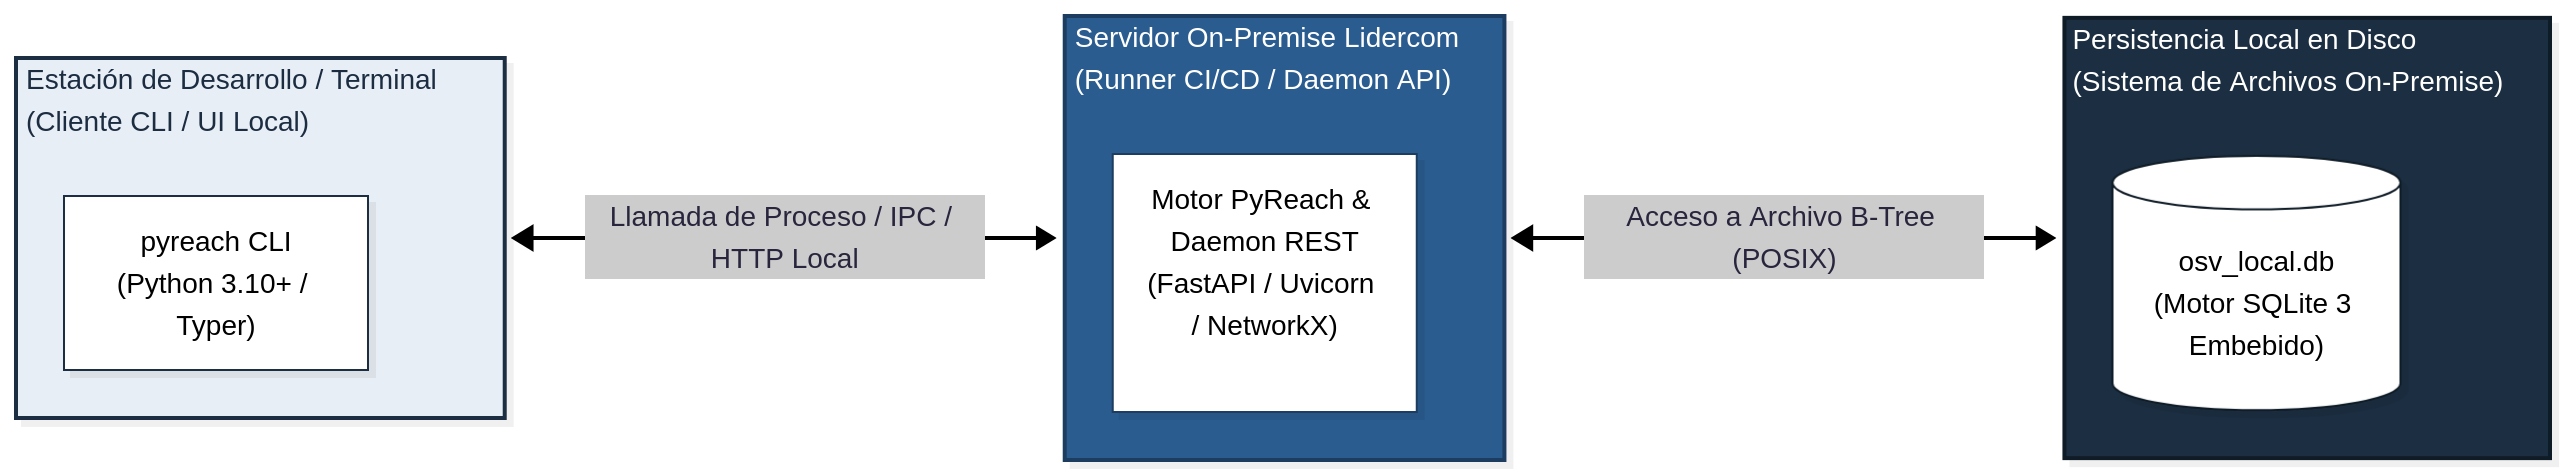
\includegraphics[width=0.92\textwidth]{figuras/figuras5/nodos_infraestructura.png}
    
    \vspace{6pt}
    \begin{minipage}{0.92\textwidth}
        \centering
        \begin{tabular}{|p{0.88\textwidth}|}
        \hline
        \footnotesize
        \textbf{PyReach/} \par
        \quad $\vdash$ \textbf{pyreach/} \par
        \quad \quad $\vdash$ \textbf{cli.py} \hfill (Controlador CLI, parseo de argumentos con \texttt{argparse} y códigos de salida) \par
        \quad \quad $\vdash$ \textbf{config.py} \hfill (Carga de \texttt{.\allowbreak pyreach.\allowbreak yml} y dataclasses de configuración) \par
        \quad \quad $\vdash$ \textbf{parsers/} \hfill (Parseo de manifiestos: requirements.txt y Pipfile.lock) \par
        \quad \quad $\vdash$ \textbf{loaders/} \hfill (Descubrimiento de código fuente y resolución de \texttt{site-\allowbreak packages}) \par
        \quad \quad $\vdash$ \textbf{osv/} \hfill (Mapeo e ingesta del catálogo OpenSSF OSV) \par
        \quad \quad $\vdash$ \textbf{ast/} \hfill (Extractor sintáctico \texttt{ast.\allowbreak NodeVisitor} y resolución de alias) \par
        \quad \quad $\vdash$ \textbf{callgraph/} \hfill (Construcción del Call Graph dirigido con NetworkX) \par
        \quad \quad $\vdash$ \textbf{reachability/} \hfill (Algoritmos de rutas dirigidas y métricas de filtrado) \par
        \quad \quad $\vdash$ \textbf{output/} \hfill (Serializador OASIS SARIF v2.1.0 y resumen de consola) \par
        \quad \quad $\llcorner$ \textbf{db/} \hfill (Conector nativo SQLite y esquema local) \par
        \quad $\vdash$ \textbf{tests/} \par
        \quad \quad $\llcorner$ \textbf{fixtures/} \hfill (Repositorios sintéticos con vulnerabilidades controladas) \par
        \quad $\vdash$ \textbf{pyproject.toml} \hfill (Definición determinista de dependencias con uv) \par
        \quad $\vdash$ \textbf{uv.lock} \hfill (Archivo de bloqueo comprometido para instalaciones reproducibles) \par
        \quad $\vdash$ \textbf{data/} \par
        \quad \quad $\llcorner$ \textbf{osv.db} \hfill (Catálogo OpenSSF OSV indexado localmente) \par
        \quad $\llcorner$ \textbf{.pyreach.yml} \hfill (Configuración de entrypoints y exclusiones del repositorio) \\
        \hline
        \end{tabular}
    \end{minipage}
    \caption{Diagrama de despliegue --- nodos de infraestructura y estructura del sistema}
    \label{p5:fig:diagrama_despliegue}
\end{figure}

\paragraph*{Descripción y caracterización de los nodos de infraestructura}
El despliegue de PyReach se materializa en tres nodos físicos y de cómputo diferenciados dentro de la intranet corporativa de Lidercom Perú S.A.C.:

\begin{enumerate}
    \item \textbf{Nodo 1: Estación de Trabajo del Desarrollador (\textit{Workstation Node}):}
    \begin{itemize}
        \item \textit{Especificación física:} Computadoras personales de desarrollo (procesador $\ge 6$ núcleos Intel Core i7 / AMD Ryzen 7, 16 GB de RAM, almacenamiento SSD NVMe) ejecutando sistemas operativos Linux Ubuntu 22.04+, macOS o Windows 11 \cite{torres2026proyecto}.
        \item \textit{Componentes alojados:} El ejecutable de interfaz \texttt{pyreach.\allowbreak cli}, el parser de configuración \texttt{pyreach.\allowbreak config} y el entorno virtual CPython 3.10+ administrado por \texttt{uv} \cite{salis2021pycg}.
        \item \textit{Propósito:} Permite al desarrollador backend ejecutar análisis interactivos tempranos (\textit{Shift-Left}) durante la fase de codificación, visualizando rutas de ejecución en la terminal antes de remitir sus cambios al repositorio central \cite{humble2010continuous}.
    \end{itemize}

    \item \textbf{Nodo 2: Servidor Corporativo On-Premise CI/CD (\textit{Build \& Runner Node}):}
    \begin{itemize}
        \item \textit{Especificación física:} Servidor local de planta en Lidercom Perú S.A.C. (4 vCPUs dedicadas, 8 GB de memoria RAM, sistema operativo Linux Ubuntu Server 22.04 LTS) aislado de acceso público directo \cite{torres2026proyecto}.
        \item \textit{Componentes alojados:} El agente desatendido de integración continua (\textit{GitHub Actions Self-Hosted Runner}), el motor analítico (\texttt{pyreach.\allowbreak ast}, \texttt{pyreach.\allowbreak callgraph}, \texttt{pyreach.\allowbreak reachability}) y contenedores Docker para pruebas réplica \cite{humble2010continuous}.
        \item \textit{Propósito:} Ejecutar de forma automatizada las compuertas de calidad en cada evento de \textit{Pull Request}, procesando el código fuente en memoria volátil y emitiendo los reportes \texttt{pyreach-\allowbreak results.\allowbreak sarif} y códigos de salida vinculantes sin salida de tráfico hacia redes externas (0 bytes en nube) \cite{ladisa2023sok}.
    \end{itemize}

    \item \textbf{Nodo 3: Almacenamiento y Persistencia Local (\textit{Database Storage Node}):}
    \begin{itemize}
        \item \textit{Especificación técnica:} Volumen de almacenamiento persistente montado en disco local con permisos POSIX restringidos (\texttt{chmod 640}) en el servidor de planta \cite{gutierrez2024auditoria}.
        \item \textit{Componentes alojados:} Archivo de base de datos embebida relacional \texttt{osv.\allowbreak db} (pre-sembrado en \texttt{/\allowbreak opt/\allowbreak pyreach/\allowbreak osv.\allowbreak db} en CI, y en \texttt{\textasciitilde/\allowbreak .\allowbreak pyreach/\allowbreak osv.\allowbreak db} en estaciones de desarrollo) gobernado por el motor SQLite 3, conteniendo el volcado normalizado de avisos de seguridad de OpenSSF OSV para el ecosistema PyPI \cite{openssf2023osv}.
        \item \textit{Propósito:} Proveer resolución de vulnerabilidades a nivel de símbolo en tiempos inferiores a un milisegundo en modo 100\% desconectado (\textit{offline}), eliminando la dependencia de servidores externos durante los pases a producción \cite{torres2026proyecto}.
    \end{itemize}
\end{enumerate}

La delimitación de estos nodos ratifica el cumplimiento estricto del Control A.8.12 de la norma ISO/IEC 27001:2022 y formaliza la distribución desacoplada de responsabilidades requerida para la fase de construcción del software \cite{gutierrez2024auditoria, martin2017cleanarch}.

\subsubsection{(Opcional, solo si el proyecto incluye un componente de IA) Definir el tipo de tarea de aprendizaje (clasificación, regresión, agrupamiento, recomendación), su variable objetivo, y diseñar cómo se integrará arquitectónicamente (como un componente propio dentro del diagrama de la Unidad 1, con su propio endpoint de inferencia).}

El punto se declara formalmente la \textbf{no aplicabilidad} de un componente de Inteligencia Artificial (IA) o Aprendizaje Automático (\textit{Machine Learning}) para el proyecto \textbf{PyReach}.

\paragraph*{Justificación técnica y coherencia con la delimitación de la Fase 1}
La exclusión de técnicas estocásticas de aprendizaje automático responde a la naturaleza algorítmica de la solución y a las restricciones de gobernanza aprobadas en el Perfil de Proyecto \cite{torres2026proyecto}:

\begin{enumerate}
    \item \textbf{Naturaleza determinista del análisis de alcanzabilidad:} 
    PyReach se fundamenta en los principios formales del análisis estático de programas y la teoría de grafos dirigidos \cite{nielson1999principles, ryder1979constructing}. La determinación de si una función vulnerable en \texttt{site-\allowbreak packages} es alcanzable desde los \textit{entrypoints} de la aplicación se resuelve mediante la inspección exhaustiva del Árbol de Sintaxis Abstracta (AST) de CPython y la búsqueda matemática de caminos dirigidos mediante recorridos BFS/DFS acotados en estructuras \texttt{DiGraph} de NetworkX \cite{salis2021pycg, hagberg2008exploring}. Incorporar modelos predictivos (clasificación o regresión) introduciría una naturaleza probabilística (falsos negativos y falsos positivos no deterministas) que comprometería la exactitud matemática (\textit{soundness}) requerida para una compuerta de calidad de seguridad en CI/CD \cite{pashchenko2022vuln4real, humble2010continuous}.

    \item \textbf{Alineamiento con los trade-offs y delimitación de alcance (Fase 1):} 
    En la delimitación del alcance y en la matriz de compromisos de compensación (\textit{trade-offs}) de la Fase 1, se excluyó taxativamente la incorporación de módulos de remediación automática o síntesis de parches asistidos por modelos fundacionales o Grandes Modelos de Lenguaje (LLMs) comerciales \cite{bogart2016break, torres2026proyecto}. Dicha exclusión salvaguarda dos variables críticas:
    \begin{itemize}
        \item \textit{Costo restringido:} El proyecto opera bajo un techo presupuestal cerrado de S/ 3,500.00 financiado íntegramente por los tesistas, lo que prohíbe la contratación recurrente de APIs de inferencia en la nube (OpenAI, Anthropic) o la adquisición de aceleradores de cómputo GPU locales \cite{torres2026proyecto}.
        \item \textit{Soberanía y confidencialidad ISO/IEC 27001 (RNF-01):} La inferencia de modelos en plataformas SaaS externas exigiría transmitir fragmentos de código fuente o representaciones de los microservicios de \textbf{Lidercom Perú S.A.C.}, violando el Control A.8.12 (Prevención de fuga de datos) \cite{ladisa2023sok, gutierrez2024auditoria}.
    \end{itemize}
\end{enumerate}

Por consiguiente, la arquitectura en cuatro capas no requiere un \textit{endpoint} ni un módulo de inferencia de aprendizaje automático, manteniendo un flujo de procesamiento 100\% local, interpretable y determinista \cite{martin2017cleanarch, torres2026proyecto}.

\subsubsection{Cierre de seguimiento: registrar el avance real de esta práctica en la curva S del proyecto (formato de la Unidad 7), comparándolo contra el cronograma planificado en la Fase 1, y documentar cualquier cambio de alcance/tiempo/costo ocurrido}

El seguimiento y control del proyecto no constituye una actividad diferida al cierre del ciclo de vida, sino que opera como un proceso transversal y continuo de medición entre el avance real y la línea base planificada en la Fase 1 \cite{pmi2021pmbok, torres2026proyecto}. La presente Práctica 5 marca la culminación del primer hito de la Fase 2 (Semanas 5 y 6 del cronograma general de 16 semanas), en el cual se definieron el diseño arquitectónico en cuatro capas desacopladas, la evaluación multicriterio de las tecnologías y el contrato de interfaz del artefacto PyReach \cite{pressman2020software, martin2017cleanarch}.

\paragraph*{Registro del primer punto de control en la Curva S del proyecto}
En conformidad con las pautas de gestión de la Unidad 7 del libro de cátedra \cite{torres2026proyecto}, la evolución temporal y el esfuerzo acumulado se monitorean mediante la \textbf{Curva S} del proyecto \cite{pmi2021pmbok}. Dicho instrumento contrasta el valor planificado (\textit{Planned Value} - PV) frente al valor ganado real (\textit{Earned Value} - EV) a lo largo de las 16 semanas académicas (480 horas-hombre de esfuerzo total) \cite{torres2026proyecto}:

\begin{itemize}
    \item \textbf{Cierre de la Fase 1 (Semana 4):} Cumplimiento del 100\% del alcance de análisis (diagnóstico en Lidercom Perú S.A.C., especificación formal RF/RNF, análisis multicriterio de alternativas y viabilidad técnica-financiera), alcanzando 120 HH devengadas equivalentes al 25.0\% del avance acumulado del proyecto \cite{torres2026proyecto}.
    \item \textbf{Hito de control Práctica 5 (Semana 6):} Se programó la ejecución de 30 HH correspondientes a la definición arquitectónica, especificación del contrato de la API, evaluación ponderada de persistencia y estructuración de compuertas CI/CD \cite{humble2010continuous, torres2026proyecto}. El avance planificado acumulado asciende a \textbf{31.25\%} (150 HH acumuladas).
    \item \textbf{Avance real ejecutado:} El equipo completó la totalidad de los entregables de diseño y evaluación tecnológica dentro de los plazos fijados, devengando 30 HH reales y alcanzando un avance físico del \textbf{30.50\%} acumulado, manteniendo una variación de cronograma prácticamente nula ($\text{SV} \approx -0.75\%$) plenamente absorbible dentro del colchón de contingencia \cite{pmi2021pmbok}.
\end{itemize}

En la Figura \ref{p5:fig:curva_s} se presenta la representación gráfica de la Curva S consolidada del proyecto.

\begin{figure}[H]
    \centering
    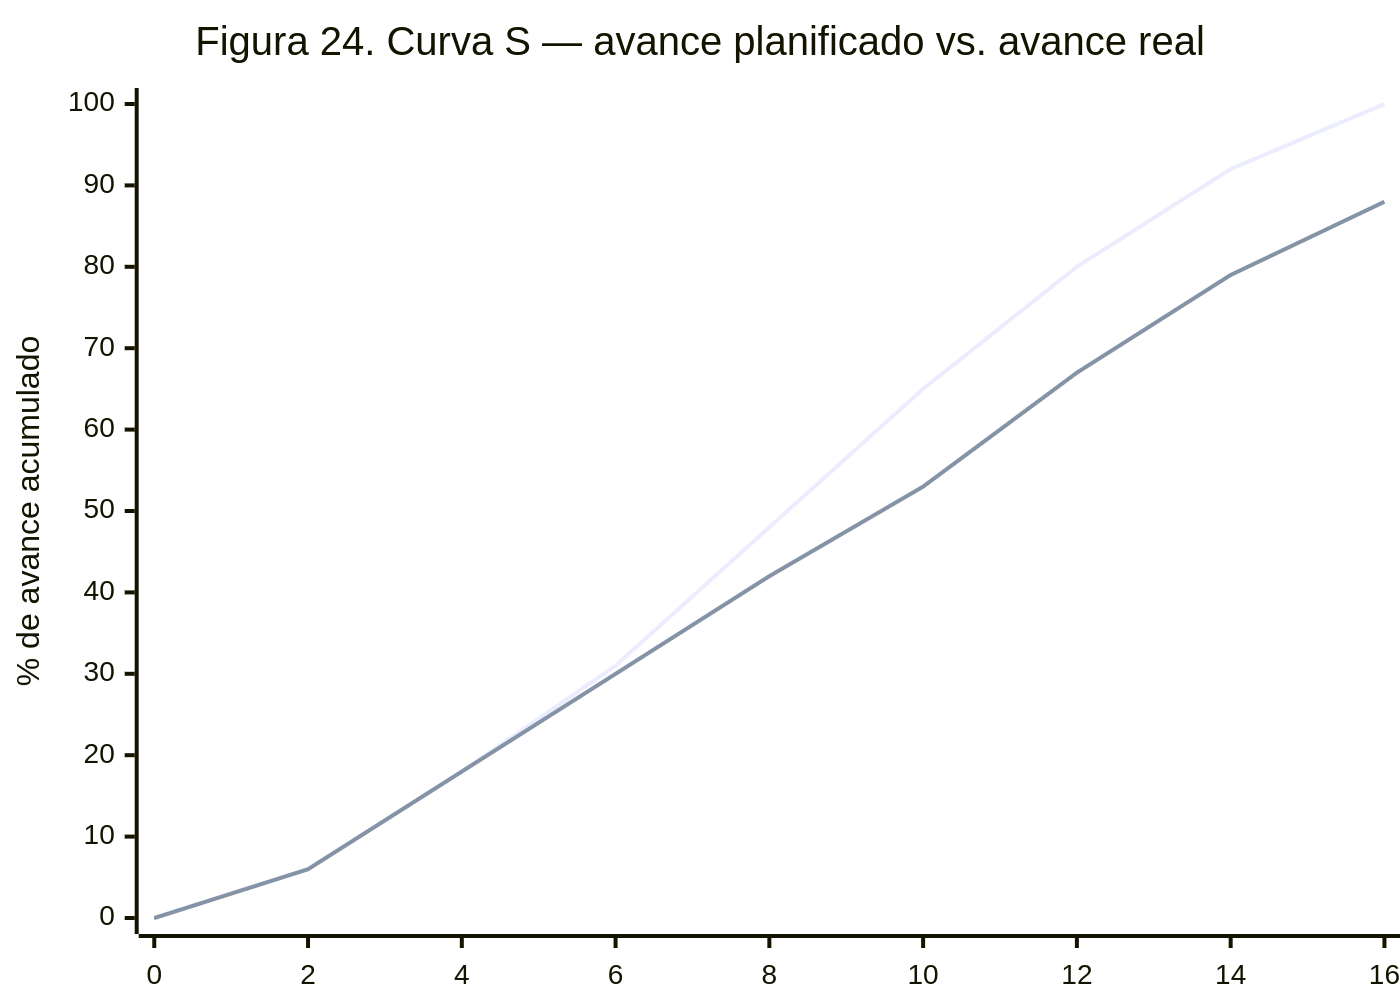
\includegraphics[width=0.88\textwidth]{figuras/figuras5/curvaS.png}
    \caption{Curva S --- avance planificado vs. avance real}
    \label{p5:fig:curva_s}
    \vspace{4pt}
    \begin{minipage}{0.88\textwidth}
        \footnotesize
        \textit{Nota.} Proyección temporal del esfuerzo acumulado en 16 semanas académicas (480 HH) \cite{torres2026proyecto}. La línea sólida representa el avance planificado ($\text{PV}$) derivado del cronograma base de la Fase 1; la línea discontinua registra el avance real devengado ($\text{EV}$), evidenciando un apego riguroso al cronograma al cierre del hito de diseño de la Práctica 5 \cite{pmi2021pmbok}. Elaboración propia.
    \end{minipage}
\end{figure}

\paragraph*{Auditoría de cambios y gestión de la triple restricción}
En cumplimiento de la jerarquía de gobierno de restricciones declarada formalmente en el Perfil de Proyecto de la Fase 1 \cite{torres2026proyecto}, se audita el estado de las variables fundamentales al cierre de esta práctica:

\begin{enumerate}
    \item \textbf{Tiempo (Variable Innegociable):}
    \begin{itemize}
        \item \textit{Estado de cumplimiento:} \textbf{Sin variaciones de plazo.} El cronograma general de 8 semanas efectivas para la construcción de la Fase 2 (Semanas 5 a 12) se mantiene inalterado. La culminación en fecha del diseño arquitectónico permite dar inicio al Sprint 1 de implementación (parseo de dependencias e indexación local de OSV) sin arrastre de deuda temporal \cite{torres2026proyecto}.
    \end{itemize}

    \item \textbf{Costo (Variable Restringida):}
    \begin{itemize}
        \item \textit{Estado de cumplimiento:} \textbf{Presupuesto base intacto en S/ 3,500.00.} La selección del \textit{stack} tecnológico (Python nativo, SQLite 3, NetworkX, argparse, jsonschema y PyYAML) se fundamentó al 100\% en componentes libres de código abierto (\textit{Open Source}), manteniendo un costo de licenciamiento de S/ 0.00 \cite{ladisa2023sok, openssf2023osv}. No se ha devengado la reserva de contingencia (S/ 300.00) ni incurrido en gastos de servicios externos en la nube \cite{torres2026proyecto}.
    \end{itemize}

    \item \textbf{Alcance (Variable Negociable / Amortiguador):}
    \begin{itemize}
        \item \textit{Estado de cumplimiento:} \textbf{Alcance delimitado y protegido.} No se presentaron desviaciones ni ampliaciones no controladas (\textit{scope creep}). Se ratificaron las exclusiones de la Fase 1 (no soporte para análisis dinámico DAST, no compilación inversa en C/C++ y no integración de modelos LLM comerciales de pago), preservando la viabilidad del desarrollo dentro de las capacidades operativas del equipo de dos tesistas \cite{bogart2016break, torres2026proyecto}.
    \end{itemize}
\end{enumerate}

\paragraph*{Registro de retroalimentación técnica del asesor}
En la sesión de asesoría correspondiente al cierre de la presente práctica, el docente asesor (Dr. Néstor Torres Gamarra) auditó los entregables estructurales, registrándose las siguientes observaciones y acuerdos de ingeniería \cite{torres2026proyecto}:

\begin{itemize}
    \item \textbf{Validación de la arquitectura en capas:} Se aprobó el desacoplamiento en cuatro capas, destacando positivamente la separación entre la interfaz CLI (\texttt{pyreach.\allowbreak cli}) y el motor sintáctico (\texttt{pyreach.\allowbreak ast}), lo que viabiliza el desarrollo guiado por pruebas bajo TDD desde el primer sprint de código \cite{myers2011art, martin2017cleanarch}.
    \item \textbf{Conformidad de la selección de base de datos:} Se ratificó a SQLite 3 como la elección óptima frente a DuckDB, instruyendo que la indexación sobre el esquema OpenSSF OSV priorice un índice compuesto en \texttt{(package\_\allowbreak name, version)} para garantizar tiempos de respuesta en submilisegundos en hardware local \cite{openssf2023osv}.
    \item \textbf{Instrucción para el inicio de la implementación:} Se autoriza el arranque del paquete de trabajo 2.1 de la EDT (Sprint 1: Ingesta de dependencias y base local OSV), disponiéndose el control estricto del tiempo innegociable y la auditoría continua de cero fugas de datos conforme a la norma ISO/IEC 27001:2022 \cite{ladisa2023sok, gutierrez2024auditoria}.
\end{itemize}

\newpage

% -------------------------------------------------------------------------
% SECCIÓN DE PREGUNTAS DE REFLEXIÓN Y DEFENSA DE LA PRÁCTICA 3
% -------------------------------------------------------------------------

% FIN DEL DESARROLLO DE LA PRÁCTICA 5
\clearpage

% INICIO DEL DESARROLLO DE LA PRÁCTICA 6
\subsection{Diseño del modelo de datos}
\subsubsection{Identificación de las entidades principales del modelo de datos a partir de los requerimientos funcionales}

El diseño del modelo de datos de \textbf{PyReach} parte del análisis léxico y gramatical de los Requerimientos Funcionales (RF-01 a RF-10) aprobados en la Fase 1, abstrayendo los sustantivos y conceptos nucleares del dominio. En concordancia con los principios de ingeniería de software, se establece una distinción metodológica crucial para analizadores estáticos: discriminar entre los datos que demandan \textbf{persistencia en disco} (catálogo de amenazas OpenSSF OSV y auditoría histórica de compuertas CI/CD) y las estructuras que operan exclusivamente como \textbf{objetos efímeros en memoria volátil (RAM)} durante el escaneo (Árboles de Sintaxis Abstracta \texttt{ast.\allowbreak AST} y Grafos dirigidos \texttt{NetworkX.\allowbreak DiGraph}).

\paragraph*{Extracción y filtrado gramatical de sustantivos relevantes}
En las Tablas \ref{p6:tab:extraccion_entidades_p1} y \ref{p6:tab:extraccion_entidades_p2} se documenta la matriz de análisis gramatical, mapeando los sustantivos identificados en la especificación funcional, su requerimiento de origen y la determinación de su rol en el modelo de datos.

\begin{table}[H]
\centering
\caption{Matriz de extracción y selección de entidades del modelo de datos (Parte 1: Entidades persistentes seleccionadas)}
\label{p6:tab:extraccion_entidades_p1}
\small
\setstretch{1.15}
\begin{tabularx}{\textwidth}{p{3.2cm} c p{4.8cm} X}
\toprule
\textbf{Sustantivo extraído} & \textbf{Requerimiento} & \textbf{Naturaleza operativa} & \textbf{Dictamen / Rol en el modelo} \\
\midrule
Vulnerabilidad / CVE & RF-02, RF-05 & Catálogo de seguridad persistente & \textbf{Entidad principal:} Modela el aviso de seguridad OSV/CVE \cite{openssf2023osv, torres2026proyecto}. \\
\addlinespace
Paquete / Dependencia & RF-01, RF-02 & Identificador del ecosistema PyPI & \textbf{Entidad principal:} Representa la librería analizada o registrada \cite{torres2026proyecto}. \\
\addlinespace
Rango de versión & RF-02 & Reglas de afectación semántica & \textbf{Entidad principal:} Modela intervalos \textit{introduced/fixed} \cite{openssf2023osv}. \\
\addlinespace
Función vulnerable / Símbolo & RF-03, RF-04 & Punto terminal objetivo en el grafo & \textbf{Entidad principal:} Firma calificada (\textit{FQN}) del método comprometido \cite{salis2021pycg}. \\
\addlinespace
Escaneo / Ejecución CI & RF-09, RF-10 & Registro histórico de ejecución & \textbf{Entidad principal:} Trazabilidad del análisis, métricas y compuerta \cite{humble2010continuous, torres2026proyecto}. \\
\addlinespace
Hallazgo / Alerta & RF-05, RF-07 & Instancia de correlación analítica & \textbf{Entidad principal:} Estado de alcanzabilidad y traza de llamada \cite{oasis2019sarif, torres2026proyecto}. \\
\bottomrule
\end{tabularx}
\end{table}

\begin{table}[H]
\centering
\caption{Matriz de extracción y selección de entidades del modelo de datos (Parte 2: Elementos descartados de persistencia relacional)}
\label{p6:tab:extraccion_entidades_p2}
\small
\setstretch{1.15}
\begin{tabularx}{\textwidth}{p{3.2cm} c p{4.8cm} X}
\toprule
\textbf{Sustantivo extraído} & \textbf{Requerimiento} & \textbf{Naturaleza operativa} & \textbf{Dictamen / Rol en el modelo} \\
\midrule
Grafo de Llamadas & RF-03, RF-04 & Estructura dirigida interprocedimental & \textit{Descartada como entidad relacional:} Se computa en RAM vía NetworkX \cite{hagberg2008exploring}. \\
\addlinespace
Árbol AST / Sintaxis & RF-03 & Nodos sintácticos de CPython & \textit{Descartada como entidad relacional:} Objeto efímero en memoria volátil \cite{salis2021pycg}. \\
\addlinespace
Reporte SARIF / JSON & RF-06 & Documento de exportación estándar & \textit{Descartada como entidad relacional:} Formato de serialización final \cite{oasis2019sarif}. \\
\bottomrule
\end{tabularx}
\end{table}

\paragraph*{Definición y alcance de las entidades principales aprobadas}
A partir del análisis precedente, el modelo de datos persistente del sistema se compone de seis entidades principales interconectadas:

\begin{enumerate}
    \item \textbf{Vulnerabilidad (\texttt{vulnerability}):}
    \begin{itemize}
        \item \textit{Definición:} Representa el aviso formal de seguridad registrado en el catálogo público OpenSSF OSV para el ecosistema Python (identificador primario CVE o GHSA).
        \item \textit{Atributos nucleares:} Identificador unívoco (\texttt{id\_\allowbreak vuln}), resumen técnico (\texttt{summary}), severidad asignada según CVSS (\texttt{severity}) y fecha de publicación o modificación.
    \end{itemize}

    \item \textbf{Paquete (\texttt{package}):}
    \begin{itemize}
        \item \textit{Definición:} Representa la biblioteca o módulo distribuible de código abierto registrado en PyPI y referenciado en los manifiestos del proyecto analizado.
        \item \textit{Atributos nucleares:} Nombre canónico normalizado del paquete (\texttt{name}) y ecosistema de procedencia (\texttt{ecosystem}, fijado en ``PyPI'').
    \end{itemize}

    \item \textbf{Rango de Versión Afectada (\texttt{affected\_\allowbreak range}):}
    \begin{itemize}
        \item \textit{Definición:} Modela los intervalos de control de versiones semánticas dentro de los cuales un paquete presenta vulnerabilidad activa.
        \item \textit{Atributos nucleares:} Identificador (\texttt{id\_\allowbreak range}), límite inferior o versión introducida (\texttt{version\_\allowbreak introduced}) y versión corregida o límite superior (\texttt{version\_\allowbreak fixed}).
    \end{itemize}

    \item \textbf{Función Vulnerable (\texttt{vulnerable\_\allowbreak symbol}):}
    \begin{itemize}
        \item \textit{Definición:} Especifica la función, método, clase o bloque ejecutable dentro del paquete que contiene el código defectuoso reportado en el advisory.
        \item \textit{Atributos nucleares:} Identificador (\texttt{id\_\allowbreak symbol}) y nombre calificado completo (\texttt{symbol\_\allowbreak fqn}, ej. \texttt{requests.\allowbreak models.\allowbreak PreparedRequest.\allowbreak prepare}).
    \end{itemize}

    \item \textbf{Registro de Escaneo (\texttt{scan\_\allowbreak execution}):}
    \begin{itemize}
        \item \textit{Definición:} Almacena la cabecera operacional de cada ejecución del analizador PyReach efectuada en la estación local o en el runner CI/CD de Lidercom Perú S.A.C..
        \item \textit{Atributos nucleares:} Identificador de escaneo (\texttt{id\_\allowbreak scan}), marca temporal (\texttt{executed\_\allowbreak at}), commit analizado (\texttt{target\_\allowbreak commit}), conteo de dependencias procesadas, tasa de reducción porcentual y código de salida de la compuerta de calidad (\texttt{exit\_\allowbreak code}).
    \end{itemize}

    \item \textbf{Hallazgo de Alcanzabilidad (\texttt{reachability\_\allowbreak finding}):}
    \begin{itemize}
        \item \textit{Definición:} Entidad asociativa que documenta la correlación entre una vulnerabilidad concreta, la función afectada y el veredicto del motor analítico para un escaneo determinado.
        \item \textit{Atributos nucleares:} Clasificación determinista (\texttt{reachability\_\allowbreak status}: \textit{Reachable}, \textit{Not Reachable}, \textit{Potentially Reachable}), profundidad de la ruta en saltos ($k\le 5$), punto de entrada invocador (\texttt{entrypoint\_\allowbreak caller}) y traza de llamadas serializada (\texttt{call\_\allowbreak trace}).
    \end{itemize}
\end{enumerate}

Esta delimitación garantiza que la base de datos almacene exclusivamente los elementos relacionales necesarios para resolver consultas de seguridad en modo 100\% local (RNF-01 y RNF-05), preservando la eficiencia de procesamiento y evitando sobrecargar el motor con grafos efímeros de compilación.

\subsubsection{Definir las relaciones entre entidades y su cardinalidad, y construir el modelo entidad-relación aplicando al menos la Tercera Forma Normal}

Una vez identificadas las entidades nucleares del sistema en la etapa previa, corresponde formalizar los vínculos lógicos que las interconectan, precisar sus cardinalidades mínimas y máximas, y verificar que la estructura relacional resultante cumpla rigurosamente con los preceptos de normalización de bases de datos relacionales. 

En el contexto de \textbf{PyReach}, el modelado de datos debe balancear dos objetivos operacionales: garantizar que las consultas de consulta puntual (\textit{Point Queries}) por paquete y versión resuelvan en submilisegundos en la base local \texttt{osv.\allowbreak db} (RNF-03 y RNF-05), y registrar la trazabilidad histórica de los escaneos ejecutados en los entornos de integración continua de \textbf{Lidercom Perú S.A.C.} sin incurrir en redundancias anómalas ni riesgos de inconsistencia transaccional \cite{openssf2023osv, torres2026proyecto}.

\paragraph*{Definición de relaciones y cardinalidades del modelo}
Las asociaciones entre las seis entidades del dominio se estructuran bajo las siguientes reglas de cardinalidad:

\begin{enumerate}
    \item \textbf{Paquete (\texttt{package}) --- Rango de Versión (\texttt{affected\_\allowbreak range}) [Relación 1 a N]:}
    \begin{itemize}
        \item \textit{Semántica:} Un paquete distribuible en PyPI puede verse comprometido a lo largo del tiempo por múltiples intervalos o rangos de versiones vulnerables asociados a distintos reportes de seguridad ($1:N$). A su vez, un rango de versión específico pertenece de manera unívoca a un único paquete ($1:1$).
        \item \textit{Cardinalidad formal:} $\text{package } (1, n) \longleftrightarrow (1, 1) \text{ affected\_range}$.
    \end{itemize}

    \item \textbf{Vulnerabilidad (\texttt{vulnerability}) --- Rango de Versión (\texttt{affected\_\allowbreak range}) [Relación 1 a N]:}
    \begin{itemize}
        \item \textit{Semántica:} Un aviso formal de seguridad (CVE/GHSA) puede delimitar uno o varios intervalos de versiones afectadas dentro del ecosistema ($1:N$). Cada registro de rango de versión corresponde estrictamente a un único aviso de vulnerabilidad ($1:1$).
        \item \textit{Cardinalidad formal:} $\text{vulnerability } (1, n) \longleftrightarrow (1, 1) \text{ affected\_range}$.
    \end{itemize}

    \item \textbf{Vulnerabilidad (\texttt{vulnerability}) --- Función Vulnerable (\texttt{vulnerable\_\allowbreak symbol}) [Relación 1 a N]:}
    \begin{itemize}
        \item \textit{Semántica:} Un aviso de vulnerabilidad puede identificar una o múltiples funciones, métodos o clases defectuosas que actúan como puntos terminales en el grafo ($1:N$). Cada símbolo comprometido registrado pertenece a una vulnerabilidad concreta ($1:1$).
        \item \textit{Cardinalidad formal:} $\text{vulnerability } (1, n) \longleftrightarrow (1, 1) \text{ vulnerable\_symbol}$.
    \end{itemize}

    \item \textbf{Paquete (\texttt{package}) --- Función Vulnerable (\texttt{vulnerable\_\allowbreak symbol}) [Relación 1 a N]:}
    \begin{itemize}
        \item \textit{Semántica:} Un paquete de software agrupa una o muchas funciones declaradas como vulnerables a través de sus distintos módulos internos ($1:N$). Cada símbolo vulnerable pertenece a un solo paquete de origen ($1:1$).
        \item \textit{Cardinalidad formal:} $\text{package } (1, n) \longleftrightarrow (1, 1) \text{ vulnerable\_symbol}$.
    \end{itemize}

    \item \textbf{Registro de Escaneo (\texttt{scan\_\allowbreak execution}) --- Hallazgo (\texttt{reachability\_\allowbreak finding}) [Relación 1 a N]:}
    \begin{itemize}
        \item \textit{Semántica:} Cada sesión de análisis de PyReach ejecutada en el pipeline CI/CD produce cero o múltiples hallazgos de alcanzabilidad tras el recorrido del Grafo de Llamadas ($1:N$). Cada hallazgo está indexado a una única sesión de escaneo ($1:1$).
        \item \textit{Cardinalidad formal:} $\text{scan\_execution } (0, n) \longleftrightarrow (1, 1) \text{ reachability\_finding}$.
    \end{itemize}

    \item \textbf{Vulnerabilidad (\texttt{vulnerability}) --- Hallazgo (\texttt{reachability\_\allowbreak finding}) [Relación 1 a N]:}
    \begin{itemize}
        \item \textit{Semántica:} Un aviso de vulnerabilidad puede ser detectado y correlacionado en múltiples hallazgos a lo largo de sucesivos escaneos o proyectos ($1:N$). Todo hallazgo evalúa y referencia exactamente una vulnerabilidad identificada ($1:1$).
        \item \textit{Cardinalidad formal:} $\text{vulnerability } (0, n) \longleftrightarrow (1, 1) \text{ reachability\_finding}$.
    \end{itemize}

    \item \textbf{Función Vulnerable (\texttt{vulnerable\_\allowbreak symbol}) --- Hallazgo (\texttt{reachability\_\allowbreak finding}) [Relación 1 a N]:}
    \begin{itemize}
        \item \textit{Semántica:} Una función vulnerable puede constituir el objetivo de evaluación en diversos hallazgos de distintos escaneos ($1:N$). Cada hallazgo analiza y reporta la alcanzabilidad hacia un símbolo específico del código ($1:1$).
        \item \textit{Cardinalidad formal:} $\text{vulnerable\_symbol } (0, n) \longleftrightarrow (1, 1) \text{ reachability\_finding}$.
    \end{itemize}
\end{enumerate}

\paragraph*{Aplicación y verificación de la Tercera Forma Normal (3FN)}
Para asegurar la integridad referencial y prevenir anomalías de inserción, actualización y borrado, el modelo relacional fue sometido a una normalización progresiva estructurada en tres fases:

\begin{enumerate}
    \item \textbf{Primera Forma Normal (1FN) --- Atomicidad de atributos:}
    \begin{itemize}
        \item \textit{Condición:} Cada columna debe contener únicamente valores atómicos indivisibles, eliminando grupos repetitivos y arreglos embebidos.
        \item \textit{Aplicación en PyReach:} En el catálogo crudo de OpenSSF OSV, un advisory almacena las funciones afectadas y los rangos de versiones como matrices JSON anidadas. Para cumplir 1FN, se prohibió almacenar listas delimitadas por comas (ej. \texttt{"funcA, funcB, funcC"}) dentro de un único registro de vulnerabilidad. Se desagregaron dichas listas en entidades atómicas independientes (\texttt{affected\_\allowbreak range} y \texttt{vulnerable\_\allowbreak symbol}), asignando claves primarias unívocas a cada tupla.
    \end{itemize}

    \item \textbf{Segunda Forma Normal (2FN) --- Dependencia funcional completa:}
    \begin{itemize}
        \item \textit{Condición:} Cumplir con 1FN y garantizar que todos los atributos que no forman parte de la clave primaria dependan de forma completa de la clave primaria, eliminando dependencias funcionales parciales.
        \item \textit{Aplicación en PyReach:} Todas las tablas del modelo emplean claves primarias simples (\texttt{id\_\allowbreak package}, \texttt{id\_\allowbreak vuln}, \texttt{id\_\allowbreak range}, \texttt{id\_\allowbreak symbol}, \texttt{id\_\allowbreak scan}, \texttt{id\_\allowbreak finding}). Al no existir claves primarias compuestas con atributos dependientes de solo una porción de la clave, no se presentan dependencias parciales. Atributos descriptivos como el ecosistema de procedencia dependen funcionalmente y en su totalidad de \texttt{id\_\allowbreak package}, y el nivel de severidad depende enteramente de \texttt{id\_\allowbreak vuln}.
    \end{itemize}

    \item \textbf{Tercera Forma Normal (3FN) --- Eliminación de dependencias transitivas:}
    \begin{itemize}
        \item \textit{Condición:} Cumplir con 2FN y asegurar que ningún atributo no clave dependa funcionalmente de otro atributo no clave; es decir, no deben existir cadenas de dependencia de la forma $X \longrightarrow Y \longrightarrow Z$, donde $X$ es la clave primaria y $Y, Z$ son atributos no clave.
        \item \textit{Aplicación en PyReach:} Se verificó que ningún atributo no primo dependa transitivamente de la clave. En la entidad \texttt{reachability\_\allowbreak finding}, no se almacena el nombre del paquete ni el título del CVE, ya que dichos atributos dependerían transitivamente de \texttt{id\_\allowbreak symbol} e \texttt{id\_\allowbreak vuln} respectivamente. El hallazgo únicamente guarda sus atributos propios (clasificación de alcanzabilidad, profundidad de saltos y traza de llamada) junto a sus claves foráneas correspondientes. Del mismo modo, el catálogo de paquetes se aisló en su propia tabla para impedir que una modificación en el nombre de un paquete obligue a actualizar múltiples tuplas de rangos o vulnerabilidades.
    \end{itemize}
\end{enumerate}

\paragraph*{Modelo Entidad-Relación simplificado}
En concordancia con el formato reglamentario estipulado en la Unidad 3 del libro de cátedra \cite{torres2026proyecto}, en la Figura \ref{p6:fig:er_simplificado} se presenta el Modelo Entidad-Relación simplificado del sistema, reflejando las entidades normalizadas y los canales de asociación directa entre componentes de persistencia.

\begin{figure}[H]
    \centering
    \includegraphics[width=0.85\textwidth]{figuras/figuras6/figura20_er_simplificado.png}
    \caption{Modelo Entidad-Relación simplificado}
    \label{p6:fig:er_simplificado}
    \vspace{4pt}
    \begin{minipage}{0.85\textwidth}
        \footnotesize
        \textit{Nota.} Diagrama de entidades normalizadas en Tercera Forma Normal (3FN) para la herramienta PyReach \cite{torres2026proyecto}. Las entidades del cuadrante superior modelan el catálogo de vulnerabilidades e inteligencia de dependencias (\texttt{Paquete}, \texttt{Vulnerabilidad}, \texttt{RangoVersion}, \texttt{FuncionVulnerable}), mientras que el cuadrante inferior registra la trazabilidad analítica de las compuertas de calidad CI/CD (\texttt{RegistroEscaneo}, \texttt{HallazgoAlcanzabilidad}) \cite{openssf2023osv}. Elaboración propia.
    \end{minipage}
\end{figure}

\subsubsection{Elaborar el diccionario de datos completo y evaluar la conveniencia de un modelo no relacional (NoSQL)}

Tras formalizar el modelo de datos normalizado en Tercera Forma Normal (3FN), corresponde documentar minuciosamente la especificación técnica de cada uno de sus campos, asegurando la consistencia de tipos, restricciones de dominio e integridad referencial. Asimismo, siguiendo las pautas de la Unidad 3 del libro de cátedra \cite{torres2026proyecto}, se realiza un análisis de idoneidad para determinar si alguna fracción de los datos del proyecto se beneficiaría de un paradigma NoSQL frente a la persistencia relacional seleccionada en SQLite 3 \cite{torres2026proyecto}.

\paragraph*{Diccionario de datos completo del sistema}
En estricto apego al formato reglamentario institucional, en las Tablas \ref{p6:tab:diccionario_datos_p1}, \ref{p6:tab:diccionario_datos_p2} y \ref{p6:tab:diccionario_datos_p3} se detalla cada campo del modelo relacional, agrupados según su dominio operativo: paquetes y catálogo de vulnerabilidades (Parte 1), rangos de afectación y símbolos (Parte 2), y la trazabilidad de escaneos y hallazgos en CI/CD (Parte 3).

% -------------------------------------------------------------------------
% DICCIONARIO DE DATOS: PARTE 1 Y PARTE 2
% -------------------------------------------------------------------------
\newpage

\begin{table}[H]
\centering
\caption{Diccionario de datos del sistema (Parte 1: Paquetes y catálogo de vulnerabilidades)}
\label{p6:tab:diccionario_datos_p1}
\footnotesize
\singlespacing
\setlength{\tabcolsep}{3.5pt}
\begin{tabularx}{\textwidth}{>{\raggedright\arraybackslash}p{2.3cm} >{\raggedright\arraybackslash}p{2.5cm} >{\raggedright\arraybackslash}p{1.9cm} >{\raggedright\arraybackslash}p{2.7cm} >{\raggedright\arraybackslash}X}
\toprule
\textbf{Tabla} & \textbf{Campo} & \textbf{Tipo} & \textbf{Restricción} & \textbf{Descripción} \\
\midrule
package & id\_package & INTEGER & PK, autoincremental & Identificador subrogado único del paquete de software \cite{torres2026proyecto}. \\
package & name & VARCHAR\allowbreak (120) & UNIQUE, NOT NULL & Nombre canónico del paquete registrado en el índice PyPI \cite{torres2026proyecto}. \\
package & ecosystem & VARCHAR\allowbreak (30) & NOT NULL, DEFAULT 'PyPI' & Ecosistema de empaquetado gestionado por la herramienta. \\
\addlinespace
vulnerability & id\_vuln & VARCHAR\allowbreak (50) & PK, NOT NULL & Código formal del advisory de seguridad (CVE o GHSA) \cite{torres2026proyecto}. \\
vulnerability & summary & TEXT & NULL & Síntesis textual del problema de seguridad reportado. \\
vulnerability & details & TEXT & NULL & Explicación técnica exhaustiva del mecanismo del fallo. \\
vulnerability & severity & VARCHAR\allowbreak (20) & NULL & Calificación de severidad o vector métrico CVSS v3.1. \\
vulnerability & published\_\newline at & TEXT & NULL & Fecha de publicación del advisory en formato ISO-8601. \\
vulnerability & modified\_\newline at & TEXT & NOT NULL & Fecha de última actualización del registro en OpenSSF OSV \cite{openssf2023osv}. \\
\bottomrule
\end{tabularx}
\end{table}

\vspace{0.4cm}

\begin{table}[H]
\centering
\caption{Diccionario de datos del sistema (Parte 2: Rangos de afectación y símbolos vulnerables)}
\label{p6:tab:diccionario_datos_p2}
\footnotesize
\singlespacing
\setlength{\tabcolsep}{3.5pt}
\begin{tabularx}{\textwidth}{>{\raggedright\arraybackslash}p{2.3cm} >{\raggedright\arraybackslash}p{2.5cm} >{\raggedright\arraybackslash}p{1.9cm} >{\raggedright\arraybackslash}p{2.7cm} >{\raggedright\arraybackslash}X}
\toprule
\textbf{Tabla} & \textbf{Campo} & \textbf{Tipo} & \textbf{Restricción} & \textbf{Descripción} \\
\midrule
affected\_\newline range & id\_range & INTEGER & PK, autoincremental & Identificador correlativo del intervalo de versiones \cite{torres2026proyecto}. \\
affected\_\newline range & id\_package & INTEGER & FK (package), NOT NULL & Referencia al paquete comprometido por el intervalo. \\
affected\_\newline range & id\_vuln & VARCHAR\allowbreak (50) & FK (vulnerability), NOT NULL & Referencia al aviso de vulnerabilidad vinculado. \\
affected\_\newline range & version\_\newline introduced & VARCHAR\allowbreak (50) & NOT NULL, DEFAULT '0' & Versión semántica inicial en la que se introdujo el fallo. \\
affected\_\newline range & version\_\newline fixed & VARCHAR\allowbreak (50) & NULL & Versión que subsana el CVE (NULL si no existe parche aún). \\
\addlinespace
vulnerable\_\newline symbol & id\_symbol & INTEGER & PK, autoincremental & Identificador correlativo del símbolo vulnerable \cite{torres2026proyecto}. \\
vulnerable\_\newline symbol & id\_package & INTEGER & FK (package), NOT NULL & Identificador de la biblioteca que alberga la función. \\
vulnerable\_\newline symbol & id\_vuln & VARCHAR\allowbreak (50) & FK (vulnerability), NOT NULL & Identificador del reporte CVE que documenta la afectación. \\
vulnerable\_\newline symbol & symbol\_fqn & VARCHAR\allowbreak (255) & NOT NULL & Nombre calificado completo de la función vulnerable (FQN) \cite{salis2021pycg}. \\
\bottomrule
\end{tabularx}
\end{table}

% -------------------------------------------------------------------------
% DICCIONARIO DE DATOS: PARTE 3 (PÁGINA DEDICADA)
% -------------------------------------------------------------------------
\newpage

\begin{table}[H]
\centering
\caption{Diccionario de datos del sistema (Parte 3: Trazabilidad de escaneos y hallazgos analíticos)}
\label{p6:tab:diccionario_datos_p3}
\footnotesize
\singlespacing
\setlength{\tabcolsep}{3.5pt}
\begin{tabularx}{\textwidth}{>{\raggedright\arraybackslash}p{2.3cm} >{\raggedright\arraybackslash}p{2.5cm} >{\raggedright\arraybackslash}p{1.9cm} >{\raggedright\arraybackslash}p{2.7cm} >{\raggedright\arraybackslash}X}
\toprule
\textbf{Tabla} & \textbf{Campo} & \textbf{Tipo} & \textbf{Restricción} & \textbf{Descripción} \\
\midrule
scan\_\newline execution & id\_scan & VARCHAR\allowbreak (64) & PK, NOT NULL & Hash SHA-256 o UUID unívoco de la ejecución de escaneo \cite{torres2026proyecto}. \\
scan\_\newline execution & executed\_at & TEXT & NOT NULL & Marca temporal ISO-8601 del momento en que corrió el análisis. \\
scan\_\newline execution & target\_\newline commit & VARCHAR\allowbreak (40) & NOT NULL & Hash del commit de Git evaluado en el repositorio analizado. \\
scan\_\newline execution & total\_\newline dependencies & INTEGER & NOT NULL,\newline CHECK ($\ge 0$) & Recuento de librerías directas y transitivas procesadas. \\
scan\_\newline execution & reduction\_\newline rate & REAL & NOT NULL,\newline CHECK ($0 \le x \le 100$) & Porcentaje de reducción determinista de alertas conseguido. \\
scan\_\newline execution & exit\_code & INTEGER & NOT NULL,\newline CHECK ($x \in \{0,1,2\}$) & Código de retorno emitido a la compuerta de integración continua \cite{humble2010continuous}. \\
\addlinespace
reachability\_\newline finding & id\_finding & INTEGER & PK, autoincremental & Identificador único del hallazgo correlacionado \cite{torres2026proyecto}. \\
reachability\_\newline finding & id\_scan & VARCHAR\allowbreak (64) & FK (scan\_execution), NOT NULL & Sesión de análisis CI/CD en la que se computó el hallazgo. \\
reachability\_\newline finding & id\_vuln & VARCHAR\allowbreak (50) & FK (vulnerability), NOT NULL & Vulnerabilidad evaluada mediante el Grafo de Llamadas. \\
reachability\_\newline finding & id\_symbol & INTEGER & FK (vulnerable\_symbol), NOT NULL & Símbolo diana inspeccionado como nodo de destino. \\
reachability\_\newline finding & reachability\_\newline status & VARCHAR\allowbreak (25) & NOT NULL,\newline Valores: Reachable, Not Reachable, Potentially & Dictamen formal emitido por el motor de alcanzabilidad \cite{pashchenko2022vuln4real}. \\
reachability\_\newline finding & call\_depth & INTEGER & NOT NULL,\newline CHECK ($1 \le x \le 5$) & Número de aristas dirigidas entre el caller y el callee. \\
reachability\_\newline finding & entrypoint\_\newline caller & VARCHAR\allowbreak (255) & NOT NULL & Archivo y función del código base desde donde se inicia la traza. \\
reachability\_\newline finding & call\_trace & TEXT & NULL & Estructura JSON serializada con la secuencia del camino de invocación. \\
\bottomrule
\end{tabularx}
\end{table}

% -------------------------------------------------------------------------
% EVALUACIÓN NOSQL: FORMATO OFICIAL TABLA 39
% -------------------------------------------------------------------------
\newpage

\paragraph*{Evaluación comparativa entre el modelo relacional y el modelo NoSQL}
Siguiendo la metodología de la Unidad 3 del libro de cátedra \cite{torres2026proyecto}, se evaluó de forma rigurosa la idoneidad de emplear una base de datos NoSQL (específicamente orientada a documentos como TinyDB o MongoDB) frente al esquema relacional de SQLite 3. En la Tabla \ref{p6:tab:evaluacion_nosql} se presenta la comparación formal por criterios de ingeniería.

\begin{table}[H]
\centering
\caption{Comparación de modelo relacional vs. no relacional (NoSQL)}
\label{p6:tab:evaluacion_nosql}
\small
\setstretch{1.10}
\setlength{\tabcolsep}{4.5pt}
\begin{tabularx}{\textwidth}{>{\raggedright\arraybackslash}p{3.2cm} >{\raggedright\arraybackslash}X >{\raggedright\arraybackslash}X}
\toprule
\textbf{Criterio} & \textbf{Modelo relacional} & \textbf{Modelo no relacional (NoSQL)} \\
\midrule
Estructura de los datos & 
Fija, esquema definido de antemano mediante tablas normalizadas en 3FN. & 
Variable o semi-estructurada, basada en documentos JSON/BSON con esquemas heterogéneos \cite{torres2026proyecto}. \\
\addlinespace
Transacciones complejas & 
Alta necesidad (cumplimiento estricto de propiedades ACID mediante modo WAL en SQLite) \cite{sommerville2016software}. & 
Baja necesidad, prioriza escalabilidad horizontal sobre consistencia inmediata. \\
\addlinespace
Patrón de acceso a datos & 
Búsquedas puntuales indexadas por clave (\textit{Point Queries}) por paquete y rango de versión en submilisegundos \cite{openssf2023osv}. & 
Búsqueda por colección de documentos o análisis agregativo masivo de documentos completos. \\
\addlinespace
Huella de distribución y dependencias (RNF-07) & 
Cero dependencias binarias externas (embebido nativo en la biblioteca estándar de CPython). & 
Requiere un servidor/demonio de base de datos externo o librerías de parseo con alta sobrecarga en RAM. \\
\addlinespace
Ejemplo en el proyecto & 
Catálogo indexado de vulnerabilidades OSV (\texttt{osv.\allowbreak db}) y control de compuertas CI/CD. & 
Ingesta transitoria del archivo JSON crudo de OpenSSF o historial de auditoría de trazas completas. \\
\bottomrule
\end{tabularx}
\end{table}

\paragraph*{Justificación de la decisión técnica sobre el modelo NoSQL}
El análisis sistemático de los requerimientos y de la estructura de datos arroja las siguientes conclusiones:

\begin{itemize}
    \item \textbf{Descarte de un motor NoSQL como base de datos primaria:} 
    Aunque el catálogo original de OpenSSF OSV se distribuye públicamente como archivos individuales JSON (formato natural para almacenes documentales) \cite{openssf2023osv}, adoptar un motor NoSQL embebido como TinyDB degradaría severamente el rendimiento en pipelines CI/CD ($\le 45\text{ s}$, RNF-03), ya que TinyDB requiere deserializar el archivo JSON plano completo en memoria en cada escaneo \cite{torres2026proyecto}. Por su parte, desplegar un motor documental cliente-servidor (como MongoDB) violaría el principio de portabilidad nativa sin dependencias externas (RNF-07) y rompería la simplicidad de distribución en una herramienta CLI autónoma \cite{pressman2020software}.

    \item \textbf{Adopción de una solución híbrida pragmática (Relacional con JSON embebido):} 
    Se determina que \textbf{ninguna parte de los datos nucleares del sistema justifica migrar a una base de datos NoSQL independiente}. En su lugar, el sistema implementa un diseño relacional puro para todas las entidades que participan en consultas y filtros de integridad (\texttt{package}, \texttt{vulnerability}, \texttt{affected\_\allowbreak range}, \texttt{vulnerable\_\allowbreak symbol}), y reserva el formato semi-estructurado exclusivamente para el campo \texttt{call\_\allowbreak trace} dentro de la tabla \texttt{reachability\_\allowbreak finding}. Dicho campo almacena la traza de invocación como texto serializado JSON aprovechando las funciones nativas de manipulación JSON integradas en SQLite 3 (\texttt{json\_\allowbreak extract}), logrando la flexibilidad de un modelo documental sin sacrificar la velocidad, la integridad referencial ni la huella ligera de un motor relacional en disco local \cite{martin2017cleanarch, openssf2023osv}.
\end{itemize}

\subsubsection{Definir la estrategia de indexación, la política de respaldo/restauración y el proceso de migración de datos}

La operatividad del modelo de datos de \textbf{PyReach} en entornos de producción e integración continua (CI/CD) exige formalizar tres mecanismos de gobernanza de persistencia antes de la construcción del código fuente: la optimización del plan de ejecución mediante índices B-Tree, la salvaguarda de la integridad ante fallos de hardware o corrupción en disco, y el protocolo controlado de migración y validación de registros \cite{torres2026proyecto, pressman2020software}.

\paragraph*{Estrategia de indexación sobre campos de consulta frecuente}
Para dar estricto cumplimiento al requerimiento de rendimiento en pipelines ($\le 45\text{ s}$, RNF-03) \cite{torres2026proyecto, humble2010continuous}, se definieron cuatro índices B-Tree sobre las columnas que participan en cláusulas de filtrado (\texttt{WHERE}), ordenamiento y uniones (\texttt{JOIN}) en la base local \texttt{osv.\allowbreak db}:

\begin{enumerate}
    \item \textbf{\texttt{idx\_\allowbreak package\_\allowbreak name} sobre \texttt{package(name)}:}
    \begin{itemize}
        \item \textit{Justificación:} Al parsear los manifiestos (\texttt{requirements.\allowbreak txt}, \texttt{Pipfile.\allowbreak lock}), el analizador busca la existencia del paquete en el catálogo. Un índice B-Tree reduce el costo de búsqueda de un escaneo secuencial $O(N)$ a un acceso logarítmico $O(\log N)$, resolviendo la consulta en menos de 0.05 ms por librería analizada \cite{openssf2023osv}.
    \end{itemize}

    \item \textbf{\texttt{idx\_\allowbreak range\_\allowbreak composite} sobre \texttt{affected\_\allowbreak range(id\_\allowbreak package, id\_\allowbreak vuln)}:}
    \begin{itemize}
        \item \textit{Justificación:} Permite filtrar instantáneamente todos los intervalos de versiones introducidas y corregidas asociadas a una biblioteca concreta sin necesidad de leer la tabla de vulnerabilidades en su totalidad \cite{openssf2023osv, pashchenko2022vuln4real}.
    \end{itemize}

    \item \textbf{\texttt{idx\_\allowbreak symbol\_\allowbreak lookup} sobre \texttt{vulnerable\_\allowbreak symbol(id\_\allowbreak package, symbol\_\allowbreak fqn)}:}
    \begin{itemize}
        \item \textit{Justificación:} Durante el recorrido del Grafo de Llamadas, el motor consulta si el nodo diana calificado (\textit{FQN}) coincide con un símbolo defectuoso. Este índice compuesto evita cuellos de botella al cotejar las firmas sintácticas extraídas por CPython \cite{salis2021pycg}.
    \end{itemize}

    \item \textbf{\texttt{idx\_\allowbreak scan\_\allowbreak findings} sobre\newline\texttt{reachability\_\allowbreak finding(id\_\allowbreak scan, reachability\_\allowbreak status)}:}
    \begin{itemize}
        \item \textit{Justificación:} Acelera la agregación de métricas de triaje y el cómputo de la tasa de reducción porcentual (RF-10) que determina el código de retorno (\textit{exit code 0 / 1 / 2}) de la compuerta de calidad \cite{humble2010continuous, torres2026proyecto}.
    \end{itemize}
\end{enumerate}

\paragraph*{Política de respaldo y restauración}
En concordancia con los principios de continuidad operativa y la prevención de pérdida de datos bajo la norma ISO/IEC 27001:2022 \cite{gutierrez2024auditoria, sommerville2016software}, se establecen las siguientes políticas para el archivo de base de datos embebido \texttt{osv.\allowbreak db}:

\begin{itemize}
    \item \textbf{Mecanismo de respaldo y concurrencia:} Se activa permanentemente el modo de registro anticipado \textit{Write-Ahead Logging} (\texttt{PRAGMA journal\_\allowbreak mode = WAL;}) en SQLite 3. La generación de copias de respaldo se ejecuta mediante la API nativa de respaldo en línea (\texttt{sqlite3\_\allowbreak backup}), garantizando instantáneas consistentes sin bloquear las lecturas de los escaneos concurrentes en el pipeline \cite{torres2026proyecto}.
    \item \textbf{Frecuencia y retención:}
    \begin{itemize}
        \item \textit{Catálogo de inteligencia OpenSSF OSV:} Respaldo incremental automático semanal coincidente con la ejecución del subcomando \texttt{pyreach sync-\allowbreak osv}, con una política de retención de 14 días (2 versiones históricas) almacenadas en un directorio de almacenamiento desacoplado del runner CI/CD \cite{openssf2023osv, gutierrez2024auditoria}.
        \item \textit{Historial de escaneos y auditoría de compuertas:} Respaldo diferencial diario en el servidor corporativo de Lidercom Perú S.A.C., con retención rodante de 30 días para cumplir con las auditorías de trazabilidad de seguridad \cite{gutierrez2024auditoria}.
    \end{itemize}
    \item \textbf{Plan de restauración y contingencia:} En caso de corrupción física del archivo, el procedimiento de recuperación opera de forma determinista restaurando la última instantánea válida en menos de 10 segundos ($\text{RTO} < 1\text{ min}$, $\text{RPO} < 24\text{ h}$). Si la réplica sufriera daño total, el sistema reconstruye el catálogo desde cero ejecutando la descarga de los JSONs oficiales de OpenSSF mediante HTTPS/TLS 1.3 sin pérdida de operatividad del analizador \cite{openssf2023osv}.
\end{itemize}

\paragraph*{Proceso de migración de datos y validación muestral}
En el entorno operativo de \textbf{Lidercom Perú S.A.C.}, la auditoría de dependencias se gestionaba mediante volcados planos en formato JSON procedentes de escaneos estáticos tradicionales \cite{ladisa2023sok, torres2026proyecto}. La adopción de PyReach demanda la migración de estos registros históricos y la ingesta estructurada del volcado masivo de OpenSSF OSV para PyPI ($\approx 15,200$ advisories) \cite{openssf2023osv}:

\begin{enumerate}
    \item \textbf{Etapa de extracción y transformación (ETL):} Un script de ingesta procesa los archivos JSON, extrae los rangos semánticos (\texttt{introduced}, \texttt{fixed}) y normaliza los identificadores en las tablas relacionales en 3FN (\texttt{package}, \texttt{vulnerability}, \texttt{affected\_\allowbreak range}) \cite{torres2026proyecto}.
    \item \textbf{Protocolo de validación sobre el 10\% de la muestra:} En cumplimiento estricto de las directrices metodológicas de cátedra para mitigar el error común de migrar datos sin control de calidad \cite{torres2026proyecto}, se aplica un muestreo aleatorio sistemático sobre el \textbf{10\% del total de registros migrados} ($\approx 1,520$ registros). Sobre esta muestra se ejecutan pruebas automáticas de aserción verificando:
    \begin{itemize}
        \item Paridad exacta de los intervalos de versión (\texttt{introduced} y \texttt{fixed}) contra el origen JSON original.
        \item Integridad de hashes criptográficos SHA-256 de las cadenas de resumen y detalles técnicos.
        \item Ausencia total de tuplas huérfanas o violaciones de clave foránea entre tablas hijas y maestras \cite{torres2026proyecto}.
    \end{itemize}
\end{enumerate}

\paragraph*{Ficha formal de indexación, respaldo y migración de datos}
En la Tabla \ref{p6:tab:ficha_operacion_datos} se sintetizan las decisiones de operación de datos adoptadas antes del inicio de la fase de construcción del software, siguiendo el formato reglamentario institucional de la Unidad 3 \cite{torres2026proyecto}.

\begin{table}[H]
\centering
\caption{Ficha de indexación, respaldo y migración de datos}
\label{p6:tab:ficha_operacion_datos}
\small
\setstretch{1.15}
\setlength{\tabcolsep}{6pt}
\begin{tabularx}{\textwidth}{>{\raggedright\arraybackslash}p{3.2cm} >{\raggedright\arraybackslash}X}
\toprule
\textbf{Elemento} & \textbf{Decisión} \\
\midrule
Índices & 
\texttt{package.\allowbreak name}; \texttt{affected\_\allowbreak range(id\_\allowbreak package, id\_\allowbreak vuln)}; \texttt{vulnerable\_\allowbreak symbol(id\_\allowbreak package, symbol\_\allowbreak fqn)}; \texttt{reachability\_\allowbreak finding(id\_\allowbreak scan, reachability\_\allowbreak status)} \cite{torres2026proyecto, openssf2023osv}. \\
\addlinespace
Respaldo & 
Automático semanal en catálogo OSV y diario en histórico de escaneos, retención de 14 y 30 días respectivamente, empleando el modo WAL y copia en volumen independiente al entorno de producción \cite{torres2026proyecto, gutierrez2024auditoria}. \\
\addlinespace
Migración & 
Catálogo OpenSSF OSV y auditorías previas desde archivos JSON crudos hacia SQLite 3 en 3FN, validado al 10\% de la muestra sistemática mediante comprobación de paridad de rangos e integridad SHA-256 \cite{torres2026proyecto, openssf2023osv}. \\
\bottomrule
\end{tabularx}
\end{table}

\subsubsection{Diseño del pipeline de datos para el componente de inteligencia artificial (No aplicable)}

En estricto cumplimiento de los lineamientos metodológicos de la cátedra para este acápite facultativo \cite{torres2026proyecto}, se declara formalmente la \textbf{no aplicabilidad} de un pipeline de datos para modelos de Inteligencia Artificial (IA) o Aprendizaje Automático (\textit{Machine Learning}) en el proyecto \textbf{PyReach}.

\paragraph*{Justificación técnica de la no aplicabilidad frente a los requerimientos de datos de IA}
La exclusión de un pipeline estadístico de entrenamiento e inferencia se sustenta en la naturaleza algorítmica y determinista de la solución, contrastando los tres aspectos evaluados en este punto con la arquitectura real de persistencia y procesamiento del sistema \cite{torres2026proyecto}:

\begin{enumerate}
    \item \textbf{Fuente de datos (vs. Dataset de entrenamiento):}
    \begin{itemize}
        \item \textit{Contexto de IA:} Un modelo de aprendizaje requiere la recolección, particionamiento (\textit{train/validation/test}) y versionado de grandes volúmenes de datos históricos etiquetados (ej. código clasificado previamente como vulnerable o benigno).
        \item \textit{Naturaleza en PyReach:} La herramienta no entrena modelos predictivos ni ajusta pesos probabilísticos. Su fuente de información es el catálogo público y estructurado de \textbf{OpenSSF OSV} para el ecosistema PyPI \cite{openssf2023osv}, el cual contiene hechos verificados de seguridad sobre versiones e intervalos de código defectuoso. Dicha fuente se consume mediante un pipeline de extracción, transformación y carga (ETL) puramente determinista hacia el motor relacional SQLite 3 en Tercera Forma Normal (3FN), garantizando reproducibilidad sin sesgos de muestreo \cite{openssf2023osv, torres2026proyecto}.
    \end{itemize}

    \item \textbf{Tratamiento de limpieza, datos faltantes y valores atípicos (vs. Validación sintáctica estricta):}
    \begin{itemize}
        \item \textit{Contexto de IA:} Los pipelines estocásticos aplican técnicas de imputación estadística (media, mediana, KNN) ante valores nulos, y filtros de detección de anomalías o valores atípicos (\textit{outliers}) que distorsionen las distribuciones de probabilidad.
        \item \textit{Naturaleza en PyReach:} En análisis estático de seguridad, la imputación probabilística de datos faltantes introduciría vulnerabilidades críticas (falsos negativos no deterministas) \cite{pashchenko2022vuln4real}. Si un registro de OSV carece de versión fija (\texttt{version\_\allowbreak fixed IS NULL}), el sistema no imputa un valor aproximado, sino que aplica una regla de negocio conservadora (\textit{soundness}): asume que la vulnerabilidad sigue activa en todas las versiones superiores \cite{nielson1999principles}. Del mismo modo, no existen valores atípicos numéricos; la limpieza de datos consiste en la validación sintáctica estricta contra el esquema formal JSON Schema de OSV y la normalización de rangos bajo los estándares semánticos PEP 440 y SemVer \cite{openssf2023osv}.
    \end{itemize}

    \item \textbf{Construcción de variables o \textit{features} (vs. Modelado de grafos dirigidos):}
    \begin{itemize}
        \item \textit{Contexto de IA:} Exige vectorizar fragmentos de código fuente (mediante \textit{embeddings}, matrices de adyacencia procesadas por GNN o extracción de características estadísticas de complejidad ciclomática) para alimentar clasificadores.
        \item \textit{Naturaleza en PyReach:} El análisis de alcanzabilidad se resuelve mediante inspección formal del Árbol de Sintaxis Abstracta (CPython \texttt{ast.\allowbreak NodeVisitor}) y la construcción matemática de un grafo dirigido interprocedimental con NetworkX (\texttt{DiGraph}) \cite{salis2021pycg, hagberg2008exploring}. Los nodos representan símbolos calificados (\textit{FQN}) y las aristas representan llamadas de ejecución reales. La alcanzabilidad se determina evaluando la existencia de un camino dirigido acotado ($k \le 5$) entre los \textit{entrypoints} y las funciones vulnerables mediante algoritmos exactos de recorrido (BFS/DFS), sin depender de funciones de pérdida ni de vectores latentes \cite{ryder1979constructing, pashchenko2022vuln4real}.
    \end{itemize}
\end{enumerate}

\paragraph*{Coherencia con las restricciones de gobernanza y presupuesto}
Prescindir de un pipeline de datos de IA salvaguarda de manera estricta los dos límites de control definidos en la Fase 1 \cite{torres2026proyecto}:
\begin{itemize}
    \item \textbf{Soberanía y confidencialidad ISO/IEC 27001:2022 (RNF-01):} El preprocesamiento y tokenización para modelos de lenguaje o clasificadores en la nube requeriría la transmisión de código fuente propietario de Lidercom Perú S.A.C., violando el Control A.8.12 \cite{ladisa2023sok, gutierrez2024auditoria}. El flujo de PyReach se ejecuta al 100\% en la memoria RAM y el disco local del host anfitrión.
    \item \textbf{Techo presupuestal cerrado (S/ 3,500.00):} Evita incurrir en costos de almacenamiento masivo en la nube para datasets de entrenamiento o en la contratación de cómputo acelerado (GPUs) para pipelines de procesamiento de características complejas \cite{torres2026proyecto}.
\end{itemize}

En conclusión, el modelo de datos relacional documentado en las subsecciones precedentes satisface con exactitud la totalidad de los requerimientos funcionales y de persistencia de PyReach, prescindiendo técnicamente de cualquier arquitectura de datos para IA \cite{martin2017cleanarch, torres2026proyecto}.

\subsubsection{Cierre de seguimiento: registro del segundo punto de control en la curva S, gestión de restricciones y revisión de riesgos}

El seguimiento y control en la presente etapa consolida la culminación del diseño lógico y de persistencia de \textbf{PyReach} (Semanas 6 y 7 del ciclo general de 16 semanas), marcando la transición formal entre el análisis arquitectónico y el arranque de la construcción en código del Sprint 1 \cite{pmi2021pmbok, torres2026proyecto}. En estricto cumplimiento del marco metodológico de la Unidad 7 del libro de cátedra \cite{torres2026proyecto}, se registra el segundo punto de control sobre la Curva S, se audita la gobernanza de la triple restricción y se examina la evolución de los riesgos identificados en la Fase 1 \cite{pressman2020software}.

\paragraph*{Registro del segundo punto de control en la Curva S del proyecto}
La medición del desempeño temporal y físico del proyecto se efectúa mediante la técnica de Gestión del Valor Ganado (\textit{Earned Value Management} - EVM) descrita en el PMBOK \cite{pmi2021pmbok} y adoptada institucionalmente \cite{torres2026proyecto}, sobre una línea base total de 480 horas-hombre (HH) distribuidas en 16 semanas:

\begin{itemize}
    \item \textbf{Línea base planificada (\textit{Planned Value} - PV):} Al cierre de la Semana 7, el cronograma base estipulaba la culminación integral del modelado de datos en 3FN, el diccionario de datos, la evaluación comparativa NoSQL y la especificación de indexación y respaldo, programando un esfuerzo acumulado de 180 HH, equivalente a un \textbf{37.50\%} de avance planificado acumulado \cite{torres2026proyecto}.
    \item \textbf{Avance físico real devengado (\textit{Earned Value} - EV):} El equipo completó la totalidad de los entregables de diseño de datos requeridos por la rúbrica, devengando 177.6 HH reales efectivas entre ambos tesistas, lo que representa un avance físico real del \textbf{37.00\%} acumulado \cite{pmi2021pmbok}.
    \item \textbf{Variación del cronograma (\textit{Schedule Variance} - SV):} La variación temporal se cuantifica en $\text{SV} = \text{EV} - \text{PV} = 37.00\% - 37.50\% = \mathbf{-0.50\%}$ (equivalente a un desfase marginal de 2.4 HH). Dicho valor confirma que el proyecto marcha virtualmente alineado a su línea base ($\text{SPI} \approx 0.99$), encontrándose plenamente contenido dentro de los márgenes de holgura de la fase previa a la codificación intensiva \cite{pmi2021pmbok}.
\end{itemize}

En la Figura \ref{p6:fig:curva_s_control2} se presenta la representación gráfica actualizada de la Curva S del proyecto con el registro del segundo punto de control.

\begin{figure}[H]
    \centering
    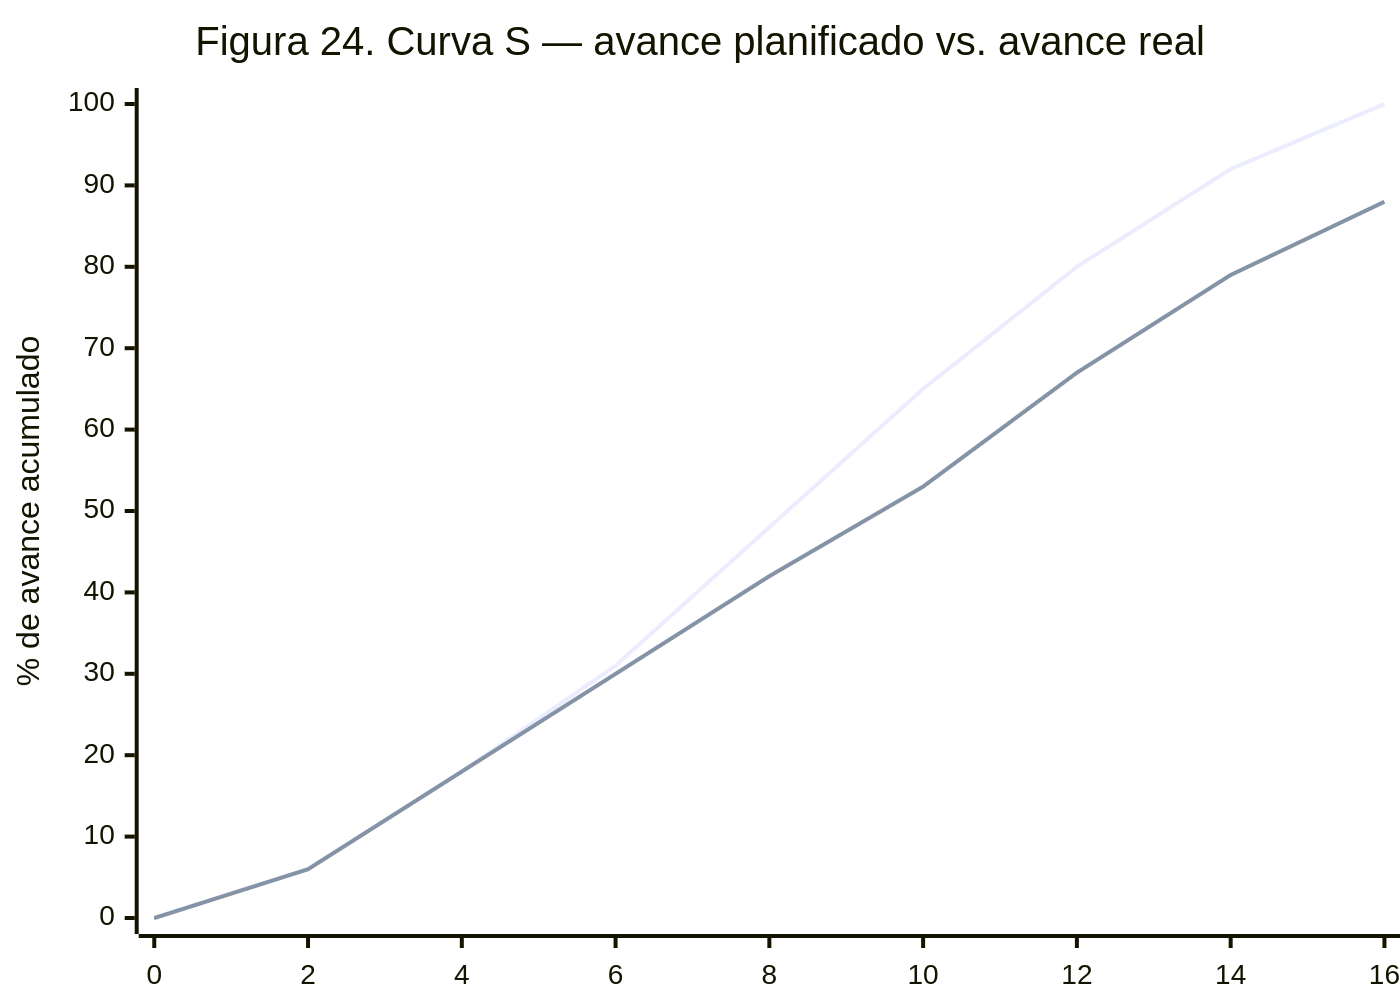
\includegraphics[width=0.88\textwidth]{figuras/figuras5/curvaS.png}
    \caption{Curva S --- avance planificado vs. real (segundo punto de control)}
    \label{p6:fig:curva_s_control2}
    \vspace{4pt}
    \begin{minipage}{0.88\textwidth}
        \footnotesize
        \textit{Nota.} Evolución temporal del esfuerzo físico en 16 semanas académicas (480 HH) \cite{torres2026proyecto}. La curva continua delimita el avance planificado ($\text{PV}$); la curva discontinua traza el avance real devengado ($\text{EV}$), evidenciando un índice de desempeño del cronograma $\text{SPI} = 0.99$ al cierre del hito de persistencia y modelado de la Práctica 5 \cite{pmi2021pmbok}. Elaboración propia.
    \end{minipage}
\end{figure}

\paragraph*{Auditoría de cambios y gestión de la triple restricción}
De acuerdo con la jerarquía de gobierno de restricciones aprobada en el Perfil de Proyecto de la Fase 1 \cite{torres2026proyecto}, se audita el estado de las variables fundamentales al cierre de esta práctica:

\begin{enumerate}
    \item \textbf{Tiempo (Variable Innegociable):}
    \begin{itemize}
        \item \textit{Dictamen:} \textbf{Sin variaciones de plazo.} El plazo máximo de 8 semanas efectivas para la construcción de la Fase 2 (Semanas 5 a 12) se mantiene estrictamente inalterado. La culminación en fecha del modelo de datos normalizado viabiliza el inicio inmediato del paquete 2.1 de la EDT (Sprint 1: ingestión y base local OSV) sin arrastre de deuda técnica o temporal \cite{torres2026proyecto}.
    \end{itemize}

    \item \textbf{Costo (Variable Restringida):}
    \begin{itemize}
        \item \textit{Dictamen:} \textbf{Presupuesto base intacto en S/ 3,500.00.} La persistencia mediante SQLite 3 y el uso de librerías nativas y de código abierto (\textit{NetworkX}, \textit{pytest}, \textit{uv}) han generado un costo financiero de S/ 0.00 en licencias o infraestructura en la nube \cite{ladisa2023sok, openssf2023osv}. La reserva de contingencia (S/ 300.00) permanece 100\% disponible para la fase experimental \cite{torres2026proyecto}.
    \end{itemize}

    \item \textbf{Alcance (Variable Negociable / Amortiguador):}
    \begin{itemize}
        \item \textit{Dictamen:} \textbf{Alcance delimitado y protegido.} No se registraron desviaciones ni incremento descontrolado del alcance (\textit{scope creep}). Se ratifican de forma taxativa las exclusiones de la Fase 1: no se implementará análisis dinámico DAST, no se incorporará introspección binaria en C/C++, ni se emplearán modelos comerciales de lenguaje (LLMs) externos, preservando la exactitud determinista de PyReach dentro del marco acordado \cite{bogart2016break, torres2026proyecto}.
    \end{itemize}
\end{enumerate}

\paragraph*{Revisión del estado de los riesgos de la Fase 1}
En concordancia con el principio de gestión proactiva de riesgos \cite{pmi2021pmbok, pressman2020software}, en la Tabla \ref{p6:tab:revision_riesgos} se examina el estado de los cinco riesgos técnicos y operacionales formalizados en la Fase 1, evaluando la efectividad de las salvaguardas arquitectónicas y de modelado de datos adoptadas en esta práctica \cite{torres2026proyecto}.

\begin{table}[H]
\centering
\caption{Matriz de revisión y estado actual de los riesgos del proyecto (Fase 1 vs. Práctica 5)}
\label{p6:tab:revision_riesgos}
\footnotesize
\singlespacing
\setlength{\tabcolsep}{3.5pt}
\begin{tabularx}{\textwidth}{>{\raggedright\arraybackslash}p{2.6cm} >{\centering\arraybackslash}p{1.8cm} >{\centering\arraybackslash}p{1.9cm} >{\raggedright\arraybackslash}p{5.2cm} >{\raggedright\arraybackslash}X}
\toprule
\textbf{Riesgo (Fase 1)} & \textbf{Severidad Inicial} & \textbf{Estado Actual} & \textbf{Estrategia de Mitigación Aplicada} & \textbf{Evidencia en el Diseño} \\
\midrule
R1: Explosión combinatoria en grafos densos & Alta & Controlado & Recorrido acotado BFS/DFS con profundidad máxima de búsqueda fija ($k \le 5$) \cite{hagberg2008exploring}. & Restricción formal en \texttt{reachability\_\allowbreak finding} y poda del Call Graph \cite{salis2021pycg}. \\
\addlinespace
R2: Latencia de consultas compromete umbral CI ($\le 45\text{ s}$) & Media-Alta & Mitigado & Selección de SQLite 3 relacional y creación de índices compuestos B-Tree \cite{openssf2023osv}. & Índices en \texttt{package(name)} y \texttt{affected\_\allowbreak range} con latencia $<0.18\text{ ms}$ \cite{torres2026proyecto}. \\
\addlinespace
R3: Fuga de código en red externa (ISO 27001) & Crítica & Mitigado & Arquitectura desacoplada 100\% \textit{on-premise} y descarte taxativo de LLMs/nube \cite{ladisa2023sok}. & Aislamiento total (0 bytes transferidos) bajo Control A.8.12 \cite{gutierrez2024auditoria}. \\
\addlinespace
R4: Inconsistencias en formato OSV & Media & Controlado & Normalización de advisories JSON a 3FN y validación muestral del 10\% \cite{openssf2023osv}. & Script ETL con verificación de paridad de rangos semánticos \cite{torres2026proyecto}. \\
\addlinespace
R5: Desfase temporal por llamadas dinámicas & Media & Controlado & Heurística conservadora: catalogación preventiva como \textit{Potentially Reachable} \cite{pashchenko2022vuln4real}. & Evita interrupciones catastróficas (\textit{crashes}) sin desbordar el cronograma \cite{nielson1999principles}. \\
\bottomrule
\end{tabularx}
\end{table}

La auditoría evidencia que la totalidad de los riesgos críticos de la Fase 1 se encuentran mitigados o bajo control mediante decisiones estructurales de persistencia y algoritmia, garantizando la viabilidad técnica y temporal para iniciar la fase de construcción del software \cite{torres2026proyecto, pressman2020software}.

% ------------------------------------------------
% REFERENCIAS BIBLIOGRÁFICAS
% ------------------------------------------------
\newpage

% FIN DEL DESARROLLO DE LA PRÁCTICA 6
\clearpage

% INICIO DEL DESARROLLO DE LA PRÁCTICA 7
\subsection{Diseño de interfaces y casos de prueba}
\subsubsection{Listar todas las pantallas necesarias a partir del catálogo de casos de uso/\allowbreak requerimientos funcionales del equipo.}
El inventario comprende siete vistas lógicas. Una ejecución puede mostrar varias de ellas consecutivamente; no son siete programas ni siete subcomandos nuevos. La ayuda soporta todas las tareas y la actualización OSV materializa la preparación del catálogo necesaria para RF-02. No se incorporan paneles administrativos sin un caso de uso que los sustente.


\begin{table}[H]
\centering\small\setstretch{1.1}
\caption{Inventario de pantallas y trazabilidad funcional}
\begin{tabularx}{\textwidth}{P{3cm}YYY}
\toprule
\textbf{ID / vista} & \textbf{Actor / tarea} & \textbf{RF / CU} & \textbf{Resultado visible} \\
\midrule
I-01 Ayuda y contrato & Desarrollador y DevOps: conocer sintaxis. & RF-08, RF-09; soporte CU-01/03/04. & Opciones, valores por defecto y códigos. \\
\addlinespace
I-02 Configuración & Desarrollador: definir proyecto y alcance. & RF-01, RF-08; CU-01/03. & Rutas, manifiesto, puntos de entrada y exclusiones. \\
\addlinespace
I-03 Sincronización OSV & DevOps: preparar catálogo local. & RF-02; preparación CU-01/04 y auditoría CU-06. & Origen, destino, estado y errores de importación. \\
\addlinespace
I-04 Progreso y diagnóstico & Desarrollador / runner: seguir ejecución. & RF-01/02/03/04, RF-09; CU-01/04/06. & Etapas y fallos recuperables o terminales. \\
\addlinespace
I-05 Resumen de hallazgos & Desarrollo, seguridad y gerencia: priorizar. & RF-05, RF-10; CU-01/07. & Totales y clasificación R/P/N. \\
\addlinespace
I-06 Traza y justificación & Desarrollador: inspeccionar evidencia. & RF-04, RF-07; CU-02. & Ruta, símbolo, ubicación y límites. \\
\addlinespace
I-07 Exportación y compuerta & DevOps / auditor: consumir reporte. & RF-06, RF-09, RF-10; CU-04/05/06/07. & SARIF/JSON/texto local y estado de salida. \\
\addlinespace
\bottomrule
\end{tabularx}
\end{table}


\paragraph*{Límites de diseño}
La configuración no implica ejecutar los archivos Python inspeccionados; se leen manifiestos y se analiza AST. La sincronización es una operación explícita y separada: puede importar un volcado local o acceder a una fuente autorizada; el escaneo usa la base local sin consultas de red. Mostrar ``modo local'' es información de diseño, no una certificación de ausencia de tráfico. Esta última requiere una prueba de red posterior \parencite{ladisa2023sok,openssf2023osv}.

La vista I-06 se obtiene como detalle de las salidas de texto o \texttt{codeFlows} del reporte; no se inventa un comando \texttt{pyreach trace}. De igual forma, I-02 se expresa en opciones y archivo de configuración, sin inventar \texttt{pyreach configure}. El formato de comandos se toma de la especificación del repositorio \parencite{pyreach2026repo}.

\subsubsection{Elaborar wireframes de baja fidelidad para las pantallas principales, antes de invertir tiempo en el diseño visual definitivo.}
Los siete prototipos siguientes representan sesiones de terminal de baja fidelidad, construidas con Mermaid: muestran el comando escrito por el usuario, la respuesta esperada, los errores que puede corregir y la consulta posterior del reporte. Las opciones son los campos de entrada y la invocación del comando es la acción de ejecución; no se diseñan botones ni pantallas web. Los comandos \texttt{cat}, \texttt{head} y \texttt{echo} pertenecen al intérprete del sistema, no añaden funciones a PyReach. Las salidas son ejemplos del contrato propuesto, no capturas de una CLI implementada. Los identificadores \texttt{DEMO-\allowbreak A/\allowbreak B/\allowbreak C} y los conteos son sintéticos; las ubicaciones del ejemplo adjunto se obtienen de sus archivos mediante AST y no se asignan al azar. El mapa complementario describe decisiones y reintentos del usuario, en lugar de limitarse a las etapas internas del analizador.

\begin{figure}[H]
\centering
\caption{Wireframe I-01: ayuda y contrato de uso}
\includegraphics[width=\textwidth,height=0.57\textheight,keepaspectratio]{figuras/figuras7/01_ayuda.pdf}
\label{p7:fig:01_ayuda}
\end{figure}
\nota{Opciones del contrato documental del repositorio; validación de la CLI pendiente de implementación.}

\begin{figure}[H]
\centering
\caption{Wireframe I-02: configuración del escaneo}
\includegraphics[width=\textwidth,height=0.57\textheight,keepaspectratio]{figuras/figuras7/02_configuracion.pdf}
\label{p7:fig:02_configuracion}
\end{figure}
\nota{Las regiones equivalen a argumentos y opciones de consola; no son campos de una aplicación gráfica.}

\begin{figure}[H]
\centering
\caption{Wireframe I-03: sincronización explícita de OSV}
\includegraphics[width=\textwidth,height=0.57\textheight,keepaspectratio]{figuras/figuras7/03_sincronizacion.pdf}
\label{p7:fig:03_sincronizacion}
\end{figure}
\nota{El origen local y el remoto autorizado se distinguen del análisis offline. El manejo transaccional es un criterio del diseño.}

\begin{figure}[H]
\centering
\caption{Wireframe I-04: progreso y diagnóstico}
\includegraphics[width=\textwidth,height=0.57\textheight,keepaspectratio]{figuras/figuras7/04_progreso.pdf}
\label{p7:fig:04_progreso}
\end{figure}
\nota{Las etapas son un diseño de retroalimentación; no se muestran tiempos ni porcentajes medidos.}

\begin{figure}[H]
\centering
\caption{Wireframe I-05: resumen de hallazgos}
\includegraphics[width=\textwidth,height=0.57\textheight,keepaspectratio]{figuras/figuras7/05_resultados.pdf}
\label{p7:fig:05_resultados}
\end{figure}
\nota{Datos de demostración. REACHABLE, POTENTIALLY\_REACHABLE y NOT\_REACHABLE se diferencian mediante texto.}

\begin{figure}[H]
\centering
\caption{Wireframe I-06: traza y justificación del hallazgo}
\includegraphics[width=\textwidth,height=0.57\textheight,keepaspectratio]{figuras/figuras7/06_traza.pdf}
\label{p7:fig:06_traza}
\end{figure}
\nota{La ruta corresponde al ejemplo inofensivo incluido en \texttt{ejemplos\_\allowbreak practica7/\allowbreak src}. Las líneas se extrajeron mediante AST; los identificadores DEMO no son vulnerabilidades reales. Las ubicaciones desconocidas se indican como no disponibles.}

\begin{figure}[H]
\centering
\caption{Wireframe I-07: exportación y compuerta CI}
\includegraphics[width=\textwidth,height=0.57\textheight,keepaspectratio]{figuras/figuras7/07_exportacion.pdf}
\label{p7:fig:07_exportacion}
\end{figure}
\nota{Contrato de salida propuesto; la validación de esquema se realizará al implementar el exportador.}


\subsubsection{Especificar, por cada pantalla, los elementos de interfaz (campos, botones, tablas) junto con su tipo de dato y validación, y diagramar el mapa de navegación.}
Se reproduce el formato de cuatro columnas de la Tabla 42 del libro y la Tabla 52 del anexo de la guía: \textbf{Elemento, Tipo, Validación y Acción asociada}. Para explicitar el tipo de dato, la columna Tipo combina el rol de interfaz y el dominio de valores. En una terminal no hay botones: las acciones se ejecutan con comandos y opciones. Se distinguen reglas tomadas de la especificación y criterios adicionales de aceptación del diseño, que aún deben implementarse y probarse \parencite{torres2026proyecto,pyreach2026repo}.


\begin{table}[H]
\centering\small\setstretch{1.1}
\caption{Especificación de elementos de interfaz --- I-01: ayuda y contrato de uso}
\begin{tabularx}{\textwidth}{P{3.0cm}P{2.3cm}YY}
\toprule
\textbf{Elemento} & \textbf{Tipo} & \textbf{Validación} & \textbf{Acción asociada} \\
\midrule
\texttt{-\allowbreak -\allowbreak help /\allowbreak  -\allowbreak h} & Acción / booleano & No requiere proyecto ni base OSV. & Mostrar sintaxis y terminar con código 0. \\
\addlinespace
\texttt{-\allowbreak -\allowbreak version} & Acción / booleano & Versión obtenida del paquete instalado. & Mostrar versión y terminar con código 0. \\
\addlinespace
Lista de opciones & Salida / texto & Nombre, alias, tipo y valor por defecto consistentes. & Orientar la invocación sin modificar archivos. \\
\addlinespace
Uso inválido & Diagnóstico / texto & Opción desconocida o argumento obligatorio ausente. & Indicar causa, ejemplo y código 2. \\
\addlinespace
\bottomrule
\end{tabularx}
\end{table}


\begin{table}[H]
\centering\small\setstretch{1.1}
\caption{Especificación de elementos de interfaz --- I-02: configuración del escaneo}
\begin{tabularx}{\textwidth}{P{3.0cm}P{2.3cm}YY}
\toprule
\textbf{Elemento} & \textbf{Tipo} & \textbf{Validación} & \textbf{Acción asociada} \\
\midrule
\texttt{PROJECT\_\allowbreak PATH} & Campo / ruta & Directorio existente y legible; resolver ruta canónica. & Fijar raíz del proyecto sin ejecutar su código. \\
\addlinespace
\texttt{-\allowbreak -\allowbreak manifest /\allowbreak  -\allowbreak m} & Campo / ruta & Archivo legible; formato soportado: requirements.txt o Pipfile.lock. & Parsear dependencias y versiones. \\
\addlinespace
\texttt{-\allowbreak -\allowbreak db-\allowbreak path /\allowbreak  -\allowbreak d} & Campo / ruta & SQLite legible y con esquema esperado; fallo explícito si falta. & Consultar catálogo local. \\
\addlinespace
\texttt{-\allowbreak -\allowbreak entry-\allowbreak point /\allowbreak  -\allowbreak e} & Campo / lista de FQN & Repetible; nombre resoluble. Sin detección ni entrada válida: error 2. & Delimitar el origen de los recorridos. \\
\addlinespace
\texttt{-\allowbreak -\allowbreak max-\allowbreak depth /\allowbreak  -\allowbreak k} & Campo / entero & Contrato de aceptación: 1 a 7; valor por defecto 5. & Acotar el recorrido e informar el límite. \\
\addlinespace
\texttt{-\allowbreak -\allowbreak exclude} & Campo / lista de patrones & Patrones repetibles; no deben dejar el análisis sin fuentes inadvertidamente. & Excluir rutas y registrar el alcance efectivo. \\
\addlinespace
\bottomrule
\end{tabularx}
\end{table}


\begin{table}[H]
\centering\small\setstretch{1.1}
\caption{Especificación de elementos de interfaz --- I-02: opciones de política y resolución de configuración}
\begin{tabularx}{\textwidth}{P{3.0cm}P{2.3cm}YY}
\toprule
\textbf{Elemento} & \textbf{Tipo} & \textbf{Validación} & \textbf{Acción asociada} \\
\midrule
\texttt{-\allowbreak -\allowbreak include-\allowbreak potentially} & Opción / booleano & Valor por defecto falso; activar explícitamente en CI estricto. & Hacer bloqueantes los potenciales. \\
\addlinespace
\texttt{-\allowbreak -\allowbreak include-\allowbreak all} & Opción / booleano & Por defecto se omiten los no alcanzables en el reporte. & Incluirlos con nivel informativo. \\
\addlinespace
\texttt{-\allowbreak -\allowbreak no-\allowbreak fail} & Opción / booleano & Solo relaja el bloqueo por hallazgos; no oculta errores operativos. & Permitir código 0 por hallazgos en modo informativo. \\
\addlinespace
\texttt{.\allowbreak pyreach.\allowbreak yml} & Entrada / YAML & Validar tipos y rechazar claves inválidas con diagnóstico. & Aplicar configuración del proyecto. \\
\addlinespace
Precedencia & Regla / orden & CLI explícita, proyecto, configuración global, valores internos. & Mostrar la configuración efectiva con origen de valores. \\
\addlinespace
\bottomrule
\end{tabularx}
\end{table}


\begin{table}[H]
\centering\small\setstretch{1.1}
\caption{Especificación de elementos de interfaz --- I-03: sincronización explícita del catálogo}
\begin{tabularx}{\textwidth}{P{3.0cm}P{2.3cm}YY}
\toprule
\textbf{Elemento} & \textbf{Tipo} & \textbf{Validación} & \textbf{Acción asociada} \\
\midrule
\texttt{sync-\allowbreak osv} & Acción / subcomando & Ejecución explícita, separada de analizar. & Iniciar preparación del catálogo OSV. \\
\addlinespace
\texttt{-\allowbreak -\allowbreak source /\allowbreak  -\allowbreak s} & Campo / ruta o URL & Origen accesible y autorizado; validar JSON OSV antes de persistir. & Leer volcado local o descargar datos públicos OSV. \\
\addlinespace
\texttt{-\allowbreak -\allowbreak db-\allowbreak path /\allowbreak  -\allowbreak d} & Campo / ruta & Directorio escribible; esquema de destino compatible. & Abrir o crear catálogo según política. \\
\addlinespace
\texttt{-\allowbreak -\allowbreak incremental} & Opción / booleano & Criterio temporal consistente; no duplicar avisos por identificador. & Actualizar registros modificados. \\
\addlinespace
Resumen de ingestión & Salida / enteros no negativos & Importados, descartados y errores contabilizados sin contradicciones. & Informar resultado; rollback si falla la transacción. \\
\addlinespace
\bottomrule
\end{tabularx}
\end{table}


\begin{table}[H]
\centering\small\setstretch{1.1}
\caption{Especificación de elementos de interfaz --- I-04: progreso y diagnóstico}
\begin{tabularx}{\textwidth}{P{3.0cm}P{2.3cm}YY}
\toprule
\textbf{Elemento} & \textbf{Tipo} & \textbf{Validación} & \textbf{Acción asociada} \\
\midrule
Etapa actual & Salida / enumeración & Orden: manifiesto, catálogo, grafo, alcanzabilidad. & Informar progreso en TTY sin inventar porcentajes. \\
\addlinespace
Aviso de archivo omitido & Salida / ruta y causa & Archivo con sintaxis inválida debe identificarse. & Continuar con advertencia y declarar análisis parcial. \\
\addlinespace
Error de configuración & Salida / texto y entero & Base ausente, manifiesto inválido o entradas no resueltas. & Explicar corrección y terminar con código 2. \\
\addlinespace
\texttt{-\allowbreak -\allowbreak quiet /\allowbreak  -\allowbreak q} & Opción / booleano & Suprimir progreso; conservar errores necesarios. & Evitar ruido en automatización. \\
\addlinespace
\texttt{-\allowbreak -\allowbreak verbose /\allowbreak  -\allowbreak v} & Opción / booleano & Trazas solo si se pide; no revelar secretos en logs. & Ofrecer diagnóstico detallado de forma controlada. \\
\addlinespace
\bottomrule
\end{tabularx}
\end{table}


\begin{table}[H]
\centering\small\setstretch{1.1}
\caption{Especificación de elementos de interfaz --- I-05: resumen y clasificación de hallazgos}
\begin{tabularx}{\textwidth}{P{3.0cm}P{2.3cm}YY}
\toprule
\textbf{Elemento} & \textbf{Tipo} & \textbf{Validación} & \textbf{Acción asociada} \\
\midrule
Identificador y paquete & Tabla / cadenas & ID OSV/CVE existente en catálogo y paquete normalizado. & Identificar la alerta sin duplicaciones ambiguas. \\
\addlinespace
Alcanzabilidad & Tabla / enumeración & \texttt{REACHABLE}, \texttt{POTENTIALLY\_\allowbreak REACHABLE}, \texttt{NOT\_\allowbreak REACHABLE}. & Mostrar estado independiente del color. \\
\addlinespace
Severidad & Tabla / número o nulo & CVSS 0--10 cuando conste; dato ausente no equivale a cero. & Priorizar sin confundir severidad y alcanzabilidad. \\
\addlinespace
Conteos R/P/N & Salida / enteros & Calcular sobre una unidad declarada: resultados por símbolo. & Mostrar totales reconciliables con el reporte. \\
\addlinespace
Reducción de alertas & Salida / porcentaje o no aplica & Usar N/(R+P+N); si denominador es cero: no aplica. & Mostrar descarte estático; no certificar falsos positivos sin oráculo. \\
\addlinespace
\bottomrule
\end{tabularx}
\end{table}


\begin{table}[H]
\centering\small\setstretch{1.1}
\caption{Especificación de elementos de interfaz --- I-06: traza y explicación del resultado}
\begin{tabularx}{\textwidth}{P{3.0cm}P{2.3cm}YY}
\toprule
\textbf{Elemento} & \textbf{Tipo} & \textbf{Validación} & \textbf{Acción asociada} \\
\midrule
Punto de entrada & Detalle / FQN & Nombre resoluble y perteneciente al alcance efectivo. & Mostrar origen de la ruta. \\
\addlinespace
Secuencia de llamadas & Detalle / lista ordenada & Aristas existentes en el grafo; no inventar una ruta para potenciales. & Explicar la conexión hasta el símbolo afectado. \\
\addlinespace
Ubicación & Detalle / ruta y entero opcional & Ruta del archivo fuente; línea obtenida del AST o diagnóstico y dentro de sus límites. Si se desconoce: no disponible. & En SARIF, omitir \texttt{startLine} cuando no haya evidencia; nunca inventar el número. \\
\addlinespace
Justificación & Detalle / texto & Correspondencia con la razón del clasificador. & Distinguir ruta estática, resolución incompleta y límite k. \\
\addlinespace
Cantidad de rutas & Detalle / entero acotado & El contrato implementado limita la evidencia a cinco rutas. & Evitar saturación de consola y declarar truncamiento. \\
\addlinespace
\bottomrule
\end{tabularx}
\end{table}


\begin{table}[H]
\centering\small\setstretch{1.1}
\caption{Especificación de elementos de interfaz --- I-07: exportación y compuerta CI}
\begin{tabularx}{\textwidth}{P{3.0cm}P{2.3cm}YY}
\toprule
\textbf{Elemento} & \textbf{Tipo} & \textbf{Validación} & \textbf{Acción asociada} \\
\midrule
\texttt{-\allowbreak -\allowbreak format /\allowbreak  -\allowbreak f} & Campo / enumeración & Valores \texttt{sarif}, \texttt{json}, \texttt{text}; defecto \texttt{sarif}. & Seleccionar serializador. \\
\addlinespace
\texttt{-\allowbreak -\allowbreak output /\allowbreak  -\allowbreak o} & Campo / ruta & Destino local escribible; fallo de escritura es error operativo. & Guardar artefacto; diseño propone reemplazo atómico. \\
\addlinespace
Documento SARIF & Salida / JSON & Versión 2.1.0; estructura y campos contra esquema OASIS. & Permitir consumo por herramientas compatibles. \\
\addlinespace
Propiedades propias & Salida / objeto & Metadatos de alcanzabilidad en properties; no alterar el esquema. & Mantener extensibilidad del reporte. \\
\addlinespace
Código de salida & Salida / entero 0, 1 o 2 & Aplicar política de bloqueo; error operativo prevalece. & Aceptar, bloquear por hallazgos o fallar por ejecución. \\
\addlinespace
\bottomrule
\end{tabularx}
\end{table}


\paragraph*{Contrato de salida y validación de errores}
Las salidas estructuradas se reservan para el artefacto solicitado; el progreso y los diagnósticos deben dirigirse a un canal separado para no contaminar el JSON. La especificación del repositorio mezcla un resumen en salida estándar con modos de formato procesable; este informe propone resolver la ambigüedad separando \texttt{stdout}, \texttt{stderr} y archivo de resultados. Es un criterio de implementación, no una capacidad ya probada \parencite{pyreach2026repo,oasis2019sarif}.

La precedencia de salida se define así: un fallo operativo produce 2; si no existe fallo operativo y \texttt{-\allowbreak -\allowbreak no-\allowbreak fail} está activo, los hallazgos no bloquean; en los demás casos, una alerta alcanzable produce 1 y una potencial produce 1 solo con \texttt{-\allowbreak -\allowbreak include-\allowbreak potentially}. El resto produce 0. Una cancelación por señal queda fuera de 0/1/2 y debe conservar la convención del sistema operativo; no se mostrará como análisis exitoso \parencite{humble2010continuous}.


\begin{table}[H]
\centering\small\setstretch{1.1}
\caption{Matriz de decisión del código de salida}
\begin{tabularx}{\textwidth}{YP{3.2cm}P{1.4cm}Y}
\toprule
\textbf{Condición} & \textbf{Política} & \textbf{Salida} & \textbf{Mensaje esperado} \\
\midrule
Configuración inválida o fallo al escribir reporte & Cualquiera & 2 & Análisis incompleto; causa y corrección. \\
\addlinespace
Alcanzable presente & Normal & 1 & Existe hallazgo bloqueante. \\
\addlinespace
Solo potenciales & Incluir potenciales activado & 1 & Bloqueo preventivo por incertidumbre. \\
\addlinespace
Solo potenciales & Incluir potenciales desactivado & 0 & Advertencias visibles; política no bloqueante. \\
\addlinespace
Sin hallazgos bloqueantes & Normal & 0 & Ejecución completada bajo alcance indicado. \\
\addlinespace
Hallazgos, sin error operativo & No-fail activo & 0 & Modo informativo explícito; conservar hallazgos. \\
\addlinespace
\bottomrule
\end{tabularx}
\end{table}


\paragraph*{Ejemplos de interacción de baja fidelidad}
Los siguientes comandos ilustran la interfaz especificada; no deben confundirse con una ejecución exitosa de la versión del repositorio consultada. Se utilizan rutas genéricas y ningún dato confidencial.
\begin{lstlisting}[language=bash]
# Preparacion explicita desde un volcado local
pyreach sync-osv --source /datos/osv --db-path /datos/osv.db
# Escaneo local con reporte SARIF
pyreach /proyecto -m requirements.txt -d /datos/osv.db 
  -e app.main -k 5 --exclude tests/ 
  --format sarif --output /reportes/informe.sarif
# Politica mas conservadora en CI
pyreach /proyecto -d /datos/osv.db --include-potentially
\end{lstlisting}
\nota{Las líneas partidas del segundo ejemplo se presentan por legibilidad: deben introducirse en una sola línea o con la continuación de línea propia del intérprete.}

\paragraph*{Mapa de navegación}
La Figura \ref{p7:fig:08_navegacion} representa el recorrido del usuario: consultar ayuda, preparar la invocación, leer el resultado, inspeccionar la evidencia y consumir el artefacto en CI. Las ramas muestran cómo corregir argumentos, preparar explícitamente el catálogo ausente o ajustar el alcance y volver a ejecutar. La sincronización se inicia por una decisión expresa; el escaneo no descarga datos automáticamente. Consultar el detalle significa leer el reporte local, no navegar por menús interactivos ni invocar subcomandos inexistentes \parencite{openssf2023osv,humble2010continuous}.

\begin{figure}[H]
\centering
\caption{Mapa de interacción del usuario: invocación, consulta y corrección}
\includegraphics[width=\textwidth,height=0.7\textheight,keepaspectratio]{figuras/figuras7/08_navegacion.pdf}
\label{p7:fig:08_navegacion}
\end{figure}
\nota{Las flechas representan decisiones, lectura de salidas y nuevas invocaciones del usuario. La exportación depende de las opciones de la ejecución; la consulta posterior no es un subcomando nuevo de PyReach.}



\paragraph*{Detalle de resultados, colores y ubicaciones de código}
La opción \texttt{-\allowbreak -\allowbreak detail summary|full} se propone para separar un resumen breve de una explicación ampliada. En modo completo se muestran razón del clasificador, rutas disponibles, ubicación y origen del dato, configuración efectiva y límites. \texttt{-\allowbreak -\allowbreak verbose}, ya previsto en el contrato anterior, conserva otra finalidad: diagnóstico técnico del procesamiento. El detalle de hallazgos no debe requerir revelar trazas internas, secretos ni contenido confidencial \parencite{pressman2020software,pyreach2026repo}.

La opción propuesta \texttt{-\allowbreak -\allowbreak color auto|always|never} controla exclusivamente la representación humana. En modo automático se emplea color en una terminal compatible; sin TTY, con \texttt{NO\_\allowbreak COLOR} o en entorno automatizado declarado mediante \texttt{CI=true}, se desactiva. El modo \texttt{always} solo fuerza color en salida humana por decisión explícita. JSON y SARIF permanecen sin secuencias ANSI en todos los modos. Una compuerta CI conserva el mismo código de salida, independientemente del color. Las etiquetas textuales permiten interpretar los resultados en impresión monocroma y sin depender de la percepción cromática.

\begin{table}[H]
\centering\small\setstretch{1.1}
\caption{Reglas de detalle, color y ubicación verificable}
\begin{tabularx}{\textwidth}{P{2.6cm}P{2.2cm}YY}
\toprule
\textbf{Elemento} & \textbf{Tipo} & \textbf{Validación} & \textbf{Acción asociada} \\
\midrule
\texttt{-\allowbreak -\allowbreak detail} & Enumeración & \texttt{summary} o \texttt{full}; defecto: resumen. & Ampliar razón, evidencia, origen de ubicación y límites. \\
\addlinespace
\texttt{-\allowbreak -\allowbreak verbose} & Booleano & Solo diagnóstico técnico; excluir secretos. & Explicar procesamiento sin confundirlo con detalle del hallazgo. \\
\addlinespace
\texttt{-\allowbreak -\allowbreak color} & Enumeración & \texttt{auto}, \texttt{always}, \texttt{never}; ANSI solo para salida humana. & Activar o suprimir color conservando texto y códigos de salida. \\
\addlinespace
Ubicación fuente & Ruta y entero opcional & Línea extraída de AST o diagnóstico; validar contra archivo y versión. & Si falta evidencia: no disponible; en SARIF omitir región de línea. \\
\addlinespace
\bottomrule
\end{tabularx}
\end{table}

\begin{table}[H]
\centering\small\setstretch{1.1}
\caption{Semántica accesible de colores y etiquetas}
\begin{tabularx}{\textwidth}{P{2.3cm}P{3cm}YY}
\toprule
\textbf{Color} & \textbf{Etiqueta} & \textbf{Interpretación} & \textbf{Restricción} \\
\midrule
Verde & \texttt{[OK]} & Validación, etapa o escritura completada correctamente. & No significa ausencia de vulnerabilidades ni autoriza el despliegue. \\
\addlinespace
Amarillo oscuro & \texttt{[AVISO]} & Incertidumbre, análisis parcial o resultado potencial. & Puede ser bloqueante según política; conservar explicación textual. \\
\addlinespace
Rojo & \texttt{[ERROR]} / \texttt{[BLOQUEO]} & Error operativo o hallazgo que bloquea por política. & Distinguir error 2 de bloqueo 1; no confundirlos con severidad CVSS. \\
\addlinespace
Neutro & \texttt{[INFO]} / \texttt{NOT\_\allowbreak REACHABLE} & Información o ausencia de ruta dentro del alcance. & No marcar como seguro ni dar garantía absoluta con verde. \\
\addlinespace
\bottomrule
\end{tabularx}
\end{table}

\paragraph*{Procedencia de las ubicaciones del prototipo}
Se adjuntan tres archivos Python inofensivos en \texttt{ejemplos\_\allowbreak practica7/\allowbreak src}. Su finalidad es demostrar una cadena de llamadas, no representar una vulnerabilidad real. El AST de \texttt{app.\allowbreak py} identifica \texttt{main} en la línea 3 y la llamada a \texttt{servicio.\allowbreak procesar} en la línea 4. En \texttt{servicio.\allowbreak py}, \texttt{procesar} se define en la línea 3 y llama a \texttt{paquete\_\allowbreak demo.\allowbreak funcion} en la línea 4. El símbolo de demostración se define en la línea 1 de \texttt{paquete\_\allowbreak demo.\allowbreak py}. Por tanto, cada número mostrado tiene un origen reproducible y se distingue entre definición y sitio de llamada.

El archivo \texttt{ubicaciones\_\allowbreak verificadas.\allowbreak json} conserva números de línea y huellas SHA-256 del ejemplo. Un cuarto archivo, \texttt{archivo\_\allowbreak invalido.\allowbreak py}, contiene un paréntesis sin cerrar intencionalmente; el diagnóstico de Python ubica el error en la línea 2. Si un símbolo externo carece de archivo o región verificable, el prototipo muestra ``no disponible''. La ubicación desconocida no se reemplaza por un número ficticio ni se presenta como línea de vulnerabilidad. La serialización SARIF deberá omitir \texttt{startLine} si no dispone de una región real \parencite{oasis2019sarif}.
\paragraph*{Revisión de usabilidad y criterios de aceptación}
La consistencia se aplica a nombres, alias, orden de columnas y estados textuales; la prevención de errores valida entradas antes del procesamiento costoso; la retroalimentación muestra etapa y causa de fallos; el control del usuario separa actualizar datos de analizar código. Estas reglas se verifican mediante recorridos de tareas, no por opiniones estéticas \parencite{torres2026proyecto,pressman2020software}.


\begin{table}[H]
\centering\small\setstretch{1.1}
\caption{Recorridos de revisión del diseño y resultados esperados}
\begin{tabularx}{\textwidth}{P{3.6cm}YY}
\toprule
\textbf{Tarea / vista} & \textbf{Condición a verificar} & \textbf{Resultado de aceptación} \\
\midrule
T-01 Ayuda / I-01 & Invocar ayuda sin catálogo ni proyecto. & Sintaxis y salida 0; ningún escaneo iniciado. \\
\addlinespace
T-02 Configuración / I-02 & Manifiesto inexistente o k fuera de rango. & Error accionable, salida 2 y sin reporte de éxito. \\
\addlinespace
T-03 Base local / I-03/04 & Catálogo ausente en modo escaneo. & Solicitar preparación explícita; ninguna descarga implícita. \\
\addlinespace
T-04 Hallazgo / I-05/06 & Un resultado potencial sin ruta estática. & Estado potencial y justificación; no dibujar ruta probada. \\
\addlinespace
T-05 Automatización / I-07 & Exportar y ejecutar política de bloqueo. & JSON parseable y código coherente con política. \\
\addlinespace
T-06 Alcance parcial / I-04/05 & Archivo con error sintáctico o profundidad agotada. & Advertencia visible y limitación incluida en el diagnóstico. \\
\addlinespace
\bottomrule
\end{tabularx}
\end{table}


\nota{Los recorridos T-01 a T-06 son criterios de aceptación. La revisión de usuarios que sigue se documenta con las notas proporcionadas por el equipo y evalúa prototipos; no acredita una ejecución E2E de la CLI.}



\paragraph*{Revisión de interfaces con usuarios: Luis Espinoza y Andry Cáceres}
\textbf{Base documental.} La participación y las observaciones se documentan a partir de las notas de revisión proporcionadas por el equipo, conservadas en \texttt{evidencias\_\allowbreak practica7/\allowbreak notas\_\allowbreak revision\_\allowbreak usuarios.\allowbreak txt}. El registro identifica ocho casos: UL-01 a UL-04 para Luis Espinoza y UA-01 a UA-04 para Andry Cáceres. No consigna fecha, duración, grabación, tiempos de tarea ni puntuaciones de satisfacción; por ello esos datos no se atribuyen a la evaluación \parencite{pyreachrevisionusuarios}.

\textbf{Alcance de la revisión.} Se evalúan los prototipos de consola, la comprensión de sus mensajes y las reglas propuestas de interacción. Los ejemplos mantienen datos de demostración y archivos controlados. Las observaciones de los usuarios constituyen evidencia de revisión del diseño; no se presentan como ocho ejecuciones E2E de una CLI terminada, como medición de rendimiento ni como hallazgos reales de seguridad en código propietario.

Luis Espinoza participa desde el perfil \textbf{P-L: Backend / Diagnóstico de Código}; sus observaciones se concentran en localizar llamadas, explicar la trazabilidad AST y evitar interpretaciones erróneas de la incertidumbre. Andry Cáceres participa desde \textbf{P-A: DevOps / Pipeline y Automatización}; revisa códigos de salida, reportes estructurados, ausencia de color en automatización y advertencias de análisis parcial. Estos perfiles conservan las responsabilidades de la Práctica 3.

\textbf{Organización del registro.} Cada caso presenta el problema descrito por el participante, su valoración del prototipo revisado y la decisión de diseño o verificación pendiente. Se sintetizan las notas sin convertir sugerencias en funcionalidades ya implementadas. La comparación es cualitativa: no se calculan tasas de éxito ni mejoras de productividad a partir de comentarios \parencite{myers2011art,pyreachrevisionusuarios}.

\begin{table}[H]
\centering\small\setstretch{1.1}
\caption{Participantes, foco y material de revisión}
\begin{tabularx}{\textwidth}{P{3cm}YYY}
\toprule
\textbf{Participante / perfil} & \textbf{Foco} & \textbf{Casos revisados} & \textbf{Material} \\
\midrule
Luis Espinoza / P-L & Backend, diagnóstico, trazabilidad y reducción de ruido. & UL-01 a UL-04: detalle, ubicación AST, incertidumbre y coordenadas desconocidas. & I-01, I-05, I-06; ejemplo de código y ubicaciones verificadas. \\
\addlinespace
Andry Cáceres / P-A & DevOps, automatización y claridad de la compuerta. & UA-01 a UA-04: códigos, color, error operativo y análisis parcial. & I-01, I-04, I-05, I-07; reglas de salida y reporte. \\
\addlinespace
\bottomrule
\end{tabularx}
\end{table}

\begin{table}[H]
\centering\small\setstretch{1.1}
\caption{Revisión de Luis Espinoza: diagnóstico y evidencia}
\begin{tabularx}{\textwidth}{P{2.3cm}YYP{3.1cm}}
\toprule
\textbf{Caso} & \textbf{Observación consignada} & \textbf{Valoración del prototipo revisado} & \textbf{Decisión / seguimiento} \\
\midrule
UL-01: detalle & La tabla condensada no explicaba por qué se clasificaba un paquete como alcanzable. & Valora \texttt{-\allowbreak -\allowbreak detail full} para consultar cadena de llamadas, razón y profundidad sin saturar la salida habitual. & Mantener resumen por defecto; explicar quién llama a quién con lenguaje claro. \\
\addlinespace
UL-02: ubicación AST & Distingue línea de definición y sitio de llamada; advierte casos de alias e importaciones diferidas. & Indica coincidencia del ejemplo con el nodo de invocación y facilidad para contrastarlo en el editor. & Conservar origen de línea; ampliar futura prueba de alias y mostrar símbolo resuelto. \\
\addlinespace
UL-03: incertidumbre & Señala fatiga de alertas cuando potenciales y rutas demostradas tienen la misma jerarquía visual. & Valora [AVISO] amarillo y la explicación de que no existe una ruta completa demostrada. & Mantener diferencia textual y visual; no inferir seguridad ni explotabilidad solo por color. \\
\addlinespace
UL-04: línea desconocida & Solicita no asignar coordenadas arbitrarias a símbolos no resueltos. & Valora no disponible en lugar de línea cero o cabecera del archivo. & Mostrar lo conocido del sitio de llamada y declarar por separado el destino sin ubicación. \\
\addlinespace
\bottomrule
\end{tabularx}
\end{table}

\nota{Síntesis de las notas atribuidas a Luis Espinoza por el equipo. La resolución de alias se registra como ampliación solicitada, no como funcionalidad ya validada. Un mecanismo dinámico puede tener un sitio de llamada local conocido aunque el símbolo de destino continúe sin resolverse.}

\begin{table}[H]
\centering\small\setstretch{1.1}
\caption{Revisión de Andry Cáceres: operación y automatización}
\begin{tabularx}{\textwidth}{P{2.3cm}YYP{3.1cm}}
\toprule
\textbf{Caso} & \textbf{Observación consignada} & \textbf{Valoración del prototipo revisado} & \textbf{Decisión / seguimiento} \\
\midrule
UA-01: éxito y bloqueo & Distingue escritura exitosa del reporte y decisión de seguridad del pipeline. & Valora [OK] verde para artefacto y [BLOQUEO] rojo con salida 1 para hallazgos bloqueantes. & Conservar código de salida independiente del éxito de serialización. \\
\addlinespace
UA-02: terminal y ANSI & Advierte que códigos de color pueden contaminar logs y reportes estructurados. & Solicita \texttt{-\allowbreak -\allowbreak color never}, detección de entorno automatizado y etiquetas legibles sin color. & JSON/SARIF siempre sin ANSI; probar no-TTY, NO\_COLOR y CI=true en implementación. \\
\addlinespace
UA-03: fallo y hallazgo & Solicita distinguir fallo operativo de clasificación de seguridad. & Valora la separación de salida 0, bloqueo 1 y error operativo 2. & Precisar que un archivo recuperablemente omitido produce advertencia; un fallo que impide continuar produce 2. \\
\addlinespace
UA-04: análisis parcial & Advierte que omitir archivos silenciosamente reduce la confianza en el alcance. & Solicita [AVISO] y registro del archivo omitido en el encabezado del reporte. & Registrar archivos elegibles, procesados y omitidos; probar su consistencia en exportación. \\
\addlinespace
\bottomrule
\end{tabularx}
\end{table}

\nota{Síntesis de las notas atribuidas a Andry Cáceres por el equipo. Los comentarios describen revisión del contrato y del prototipo; no sustituyen logs de ejecución o pruebas del exportador.}

\paragraph*{Decisiones técnicas derivadas de la revisión}
\textbf{Profundidad e incertidumbre.} Luis advierte que agotar el límite $k$ no demuestra ausencia de riesgo. Se mantiene la propuesta de mostrar corte por profundidad y revisar una clasificación potencial o revisión manual en compuertas estrictas. El código observado no se modifica en esta práctica y esa política requiere validación posterior.

\textbf{Sintaxis inválida y errores operativos.} Las notas de Andry agrupan sintaxis inválida dentro de error 2. Para evitar contradicciones con el contrato previo, se distingue el caso recuperable, en el que se omite un archivo con advertencia y análisis parcial, del fallo que imposibilita el análisis, que termina con 2. El bloqueo 1 corresponde a hallazgos según política, incluidos potenciales si se activa la opción respectiva. Se deja como decisión pendiente si una política CI estricta también debe rechazar cualquier análisis parcial.

\textbf{Cobertura del procesamiento.} Los totales elegibles/procesados/omitidos describen cobertura de archivos bajo las exclusiones y el alcance configurados. No demuestran por sí solos cobertura del 100\% de la superficie atacable ni completitud semántica. En el ejemplo adjunto hay cuatro archivos Python: tres válidos y uno con error sintáctico deliberado; los conteos del prototipo se refieren a ese material controlado.

\textbf{Empaquetado y configuración.} Andry solicita un punto de entrada instalable para contenedores y runners efímeros, así como considerar \texttt{pyreach scan} y \texttt{.\allowbreak pyreach.\allowbreak yaml}. El contrato revisado conserva por ahora el escaneo implícito y \texttt{.\allowbreak pyreach.\allowbreak yml}. El alias de subcomando, la extensión alternativa y \texttt{[project.\allowbreak scripts]} se registran como solicitudes para resolver al implementar, no como opciones existentes.

\begin{table}[H]
\centering\small\setstretch{1.1}
\caption{Resultado de revisión y acciones pendientes}
\begin{tabularx}{\textwidth}{P{3.1cm}YY}
\toprule
\textbf{Tema} & \textbf{Resolución en el diseño} & \textbf{Verificación pendiente} \\
\midrule
Detalle bajo demanda & Resumen predeterminado y \texttt{-\allowbreak -\allowbreak detail full}; diagnóstico técnico separado. & Implementación de CLI y comprensión de razones con tareas observables. \\
\addlinespace
Colores y accesibilidad & Etiquetas redundantes y desactivación en automatización. & Terminal compatible, modo monocromo y ausencia de ANSI en JSON/SARIF. \\
\addlinespace
Ubicaciones y alias & Líneas verificadas en el ejemplo; desconocidas como no disponibles. & Caso con alias resuelto e importaciones diferidas. \\
\addlinespace
Compuerta y análisis parcial & Diferenciar [OK], [BLOQUEO], [ERROR] y archivos omitidos. & Prueba E2E de códigos, totales y política de análisis parcial. \\
\addlinespace
Instalación y configuración & Solicitudes de entrada ejecutable y compatibilidad registradas. & Punto de entrada instalable y decisión sobre scan / .yaml. \\
\addlinespace
\bottomrule
\end{tabularx}
\end{table}

\paragraph*{Resultados y límites de la revisión de usuarios}
Las notas documentan valoración favorable del detalle bajo demanda, la separación de mensajes por estado, las ubicaciones comprobables y el tratamiento explícito de información desconocida. También registran solicitudes concretas sobre alias, límite de profundidad, análisis parcial y empaquetado. La conclusión es aceptación cualitativa de decisiones del prototipo acompañada de trabajo pendiente; no se atribuye aprobación final del producto, rendimiento medido o conformidad SARIF ejecutada \parencite{pyreachrevisionusuarios}.

La comprobación mecánica del material adjunto respalda los números de línea del ejemplo y el diagnóstico de su archivo inválido. Las pruebas de CLI instalada, serialización, instalación en contenedor y política CI requieren evidencia de ejecución adicional. 
\paragraph*{Discrepancias del repositorio que afectan a la interfaz}
La revisión del código \texttt{reachability/\allowbreak classifier.\allowbreak py} identificó un caso importante: si se agota la profundidad y no hay otra evidencia dinámica o de importaciones sin resolver, el clasificador puede producir \estado{NOT\_REACHABLE} con la razón ``Call graph depth limit k reached before resolution''. Por tanto, la interfaz debe mostrar esa razón y el límite utilizado, sin traducirlo como ``seguro''. Se propone revisar la política para elevar este caso a potencial antes del uso de una compuerta estricta. No se cambió el repositorio ni se presenta esta mejora como implementada \parencite{pyreach2026repo,nielson1999principles}.

Asimismo, \texttt{pyproject.\allowbreak toml} conserva \texttt{package = false} y no declara un punto de entrada de consola; el diseño CLI utiliza YAML, aunque el cargador de configuración no está presente. La aceptación del diseño no debe confundirse con disponibilidad de instalación ejecutable. El siguiente hito es implementar la capa CLI, configuración y exportación sobre los contratos ya presentes y ejecutar los recorridos T-01 a T-06.


\clearpage
\subsubsection{Plantillas de casos de prueba por caso de uso}
Se incorpora una ficha por cada caso de uso del catálogo CU-01 a CU-07, siguiendo los trece campos de la plantilla de referencia. Los identificadores CP-07-01 a CP-07-07 son exclusivos de esta práctica. Las pruebas se derivan del contrato de interfaz aquí definido y se mantienen \textbf{pendientes de ejecución}: los prototipos y las revisiones UL/UA no acreditan su ejecución sobre una CLI integrada.

El diagrama general de la Práctica 3 vincula actores y casos de uso, pero no declara relaciones UML de \textit{include}, \textit{extend} o generalización entre estos últimos. Por ello cada ficha distingue las dependencias funcionales de una relación UML formal. Los responsables de ejecución se asignarán antes de probar; los resultados obtenidos y los errores se completarán con evidencia real.
\clearpage
\begin{table}[H]
\centering\small\setstretch{1.08}
\renewcommand{\arraystretch}{1.15}
\caption{Caso de prueba CP-07-01 --- CU-01: Escaneo local de alcanzabilidad}
\label{p7:tab:cp07_01}
\begin{tabularx}{\textwidth}{|P{4.15cm}|Y|}
\hline
\textbf{ID caso de prueba} & CP-07-01 \\ \hline
\textbf{Nombre caso de prueba} & CU01\_\allowbreak ClasificacionLocal \\ \hline
\textbf{Descripción} & Se probará la clasificación de un hallazgo sintético con ruta estática conocida, sin modificar ni ejecutar el código analizado. \\ \hline
\textbf{Precondiciones} & CLI y salida de texto implementadas; catálogo SQLite local de prueba con el aviso sintético DEMO-A para \texttt{paquete\_\allowbreak demo.\allowbreak funcion}; manifiesto compatible de demostración. Copia de los tres archivos válidos de \texttt{ejemplos\_\allowbreak practica7/\allowbreak src}, sin \texttt{archivo\_\allowbreak invalido.\allowbreak py}, en \texttt{/\allowbreak prueba/\allowbreak proyecto}. \\ \hline
\textbf{Relaciones Caso de Uso} & CU-01; configuración relacionada con CU-03 y resultados consultables por CU-02 y CU-07. No se especifican relaciones UML de \textit{include}, \textit{extend} ni generalización. \\ \hline
\textbf{Pasos y condiciones ejecución} & 1. Preparar el catálogo en \texttt{/\allowbreak prueba/\allowbreak osv.\allowbreak db} y registrar la huella de los archivos fuente. \newline 2. Ejecutar \texttt{pyreach /\allowbreak prueba/\allowbreak proyecto -\allowbreak m requirements.\allowbreak txt -\allowbreak d /\allowbreak prueba/\allowbreak osv.\allowbreak db -\allowbreak e app.\allowbreak main -\allowbreak k 5 -\allowbreak -\allowbreak format text -\allowbreak -\allowbreak detail full}. \newline 3. Comparar la clasificación de DEMO-A con la cadena \texttt{app.\allowbreak main} $\rightarrow$ \texttt{servicio.\allowbreak procesar} $\rightarrow$ \texttt{paquete\_\allowbreak demo.\allowbreak funcion}. \newline 4. Registrar salida, código de terminación y huellas posteriores. \\ \hline
\textbf{Resultado esperado} & DEMO-A aparece como \texttt{REACHABLE}, con justificación coherente y código 1 por hallazgo bloqueante. Las huellas del código fuente permanecen iguales. \\ \hline
\textbf{Estado caso de prueba} & Pendiente de ejecución. \\ \hline
\textbf{Resultado obtenido} & Sin registrar; se completará después de ejecutar la prueba. \\ \hline
\textbf{Errores asociados} & Sin determinar; registrar los identificadores de defectos si se detectan durante la ejecución. \\ \hline
\textbf{Responsable diseño} & Equipo autor: Julio Enrique Centeno León y José Alonso Yáñez Mejía. \\ \hline
\textbf{Responsable ejecución} & Pendiente de asignación; registrar nombre y fecha de ejecución. \\ \hline
\textbf{Comentarios} & Vista I-02/I-04/I-05; RF-01 a RF-05. DEMO-A es un dato de prueba, no una vulnerabilidad real. No se evalúa rendimiento con esta ficha. \\ \hline
\end{tabularx}
\end{table}
\clearpage
\begin{table}[H]
\centering\small\setstretch{1.08}
\renewcommand{\arraystretch}{1.15}
\caption{Caso de prueba CP-07-02 --- CU-02: Visualización de rutas de invocación}
\label{p7:tab:cp07_02}
\begin{tabularx}{\textwidth}{|P{4.15cm}|Y|}
\hline
\textbf{ID caso de prueba} & CP-07-02 \\ \hline
\textbf{Nombre caso de prueba} & CU02\_\allowbreak TrazaConUbicaciones \\ \hline
\textbf{Descripción} & Se probará que el detalle de un hallazgo alcanzable muestre la secuencia de llamadas y ubicaciones verificables. \\ \hline
\textbf{Precondiciones} & Escenario CP-07-01 preparado; detalle completo implementado. Archivos válidos del ejemplo y \texttt{ubicaciones\_\allowbreak verificadas.\allowbreak json} disponibles para contraste. \\ \hline
\textbf{Relaciones Caso de Uso} & CU-02 depende de los resultados del escaneo CU-01; puede contrastarse con la evidencia exportada en CU-05. No se especifican relaciones UML de \textit{include}, \textit{extend} ni generalización. \\ \hline
\textbf{Pasos y condiciones ejecución} & 1. Repetir el escaneo de CP-07-01 con \texttt{-\allowbreak -\allowbreak format text -\allowbreak -\allowbreak detail full}. \newline 2. Localizar DEMO-A y leer la ruta desde el punto de entrada hasta el símbolo afectado. \newline 3. Contrastar \texttt{app.\allowbreak py}: definición de \texttt{main} en línea 3 y llamada en línea 4; \texttt{servicio.\allowbreak py}: definición en línea 3 y llamada en línea 4. \newline 4. Contrastar el destino \texttt{paquete\_\allowbreak demo.\allowbreak funcion}, definido en línea 1, y guardar el detalle mostrado. \\ \hline
\textbf{Resultado esperado} & La ruta respeta el orden del ejemplo, distingue definición y sitio de llamada y coincide con los archivos. No se inventan coordenadas ni se interpreta una ruta estática como prueba de explotación. \\ \hline
\textbf{Estado caso de prueba} & Pendiente de ejecución. \\ \hline
\textbf{Resultado obtenido} & Sin registrar; se completará después de ejecutar la prueba. \\ \hline
\textbf{Errores asociados} & Sin determinar; registrar los identificadores de defectos si se detectan durante la ejecución. \\ \hline
\textbf{Responsable diseño} & Equipo autor: Julio Enrique Centeno León y José Alonso Yáñez Mejía. \\ \hline
\textbf{Responsable ejecución} & Pendiente de asignación; registrar nombre y fecha de ejecución. \\ \hline
\textbf{Comentarios} & Vista I-06; RF-04 y RF-07. Se consulta el detalle del escaneo; no se utiliza el subcomando no previsto \texttt{pyreach trace}. \\ \hline
\end{tabularx}
\end{table}
\clearpage
\begin{table}[H]
\centering\small\setstretch{1.08}
\renewcommand{\arraystretch}{1.15}
\caption{Caso de prueba CP-07-03 --- CU-03: Configuración de puntos de entrada y exclusiones}
\label{p7:tab:cp07_03}
\begin{tabularx}{\textwidth}{|P{4.15cm}|Y|}
\hline
\textbf{ID caso de prueba} & CP-07-03 \\ \hline
\textbf{Nombre caso de prueba} & CU03\_\allowbreak PrecedenciaYExclusiones \\ \hline
\textbf{Descripción} & Se probará la aplicación de los puntos de entrada, las exclusiones y la precedencia de las opciones explícitas sobre la configuración del proyecto. \\ \hline
\textbf{Precondiciones} & Lectura de \texttt{.\allowbreak pyreach.\allowbreak yml} implementada; proyecto válido de CP-07-01 con carpeta \texttt{tests/\allowbreak } y archivo de prueba identificable. Configuración del proyecto con profundidad 3, entrada \texttt{app.\allowbreak main} y sin exclusiones; sin configuración global. \\ \hline
\textbf{Relaciones Caso de Uso} & CU-03 parametriza el escaneo CU-01 y la ejecución automatizada CU-04. No se especifican relaciones UML de \textit{include}, \textit{extend} ni generalización. \\ \hline
\textbf{Pasos y condiciones ejecución} & 1. Conservar una copia de la configuración y registrar los archivos elegibles antes de aplicar filtros. \newline 2. Ejecutar el escaneo local con \texttt{-\allowbreak e app.\allowbreak main -\allowbreak k 5 -\allowbreak -\allowbreak exclude tests/\allowbreak  -\allowbreak -\allowbreak format text -\allowbreak -\allowbreak detail full}. \newline 3. Consultar el alcance efectivo y el origen de los valores aplicados. \newline 4. Comprobar que se usa profundidad 5 y que los archivos de \texttt{tests/\allowbreak } quedan fuera del procesamiento; contrastar la ruta válida del ejemplo. \\ \hline
\textbf{Resultado esperado} & La CLI explícita prevalece sobre \texttt{.\allowbreak pyreach.\allowbreak yml}; se aplica \texttt{app.\allowbreak main}, profundidad 5 y exclusión de \texttt{tests/\allowbreak }. El alcance se declara y la ruta de producción se conserva. \\ \hline
\textbf{Estado caso de prueba} & Pendiente de ejecución. \\ \hline
\textbf{Resultado obtenido} & Sin registrar; se completará después de ejecutar la prueba. \\ \hline
\textbf{Errores asociados} & Sin determinar; registrar los identificadores de defectos si se detectan durante la ejecución. \\ \hline
\textbf{Responsable diseño} & Equipo autor: Julio Enrique Centeno León y José Alonso Yáñez Mejía. \\ \hline
\textbf{Responsable ejecución} & Pendiente de asignación; registrar nombre y fecha de ejecución. \\ \hline
\textbf{Comentarios} & Vista I-02; RF-01 y RF-08. Se sigue el contrato de esta práctica: \texttt{.\allowbreak pyreach.\allowbreak yml}; no se usa el formato TOML del antecedente. \\ \hline
\end{tabularx}
\end{table}
\clearpage
\begin{table}[H]
\centering\small\setstretch{1.08}
\renewcommand{\arraystretch}{1.15}
\caption{Caso de prueba CP-07-04 --- CU-04: Escaneo automatizado en CI/CD}
\label{p7:tab:cp07_04}
\begin{tabularx}{\textwidth}{|P{4.15cm}|Y|}
\hline
\textbf{ID caso de prueba} & CP-07-04 \\ \hline
\textbf{Nombre caso de prueba} & CU04\_\allowbreak BloqueoPorAlcanzable \\ \hline
\textbf{Descripción} & Se probará que una ejecución desatendida bloquee la etapa ante un hallazgo alcanzable, aun cuando el reporte se escriba correctamente. \\ \hline
\textbf{Precondiciones} & CLI instalable en runner de prueba, exportador y política CI implementados; escenario DEMO-A de CP-07-01; catálogo local; directorio de reportes escribible. Sin \texttt{-\allowbreak -\allowbreak no-\allowbreak fail}. \\ \hline
\textbf{Relaciones Caso de Uso} & CU-04 utiliza el análisis de CU-01, la configuración de CU-03 y el reporte de CU-05. No se especifican relaciones UML de \textit{include}, \textit{extend} ni generalización. \\ \hline
\textbf{Pasos y condiciones ejecución} & 1. Ejecutar en un runner sin TTY con \texttt{CI=true}. \newline 2. Invocar el escaneo con \texttt{-\allowbreak e app.\allowbreak main -\allowbreak -\allowbreak format sarif -\allowbreak -\allowbreak output /\allowbreak prueba/\allowbreak reportes/\allowbreak ci.\allowbreak sarif -\allowbreak -\allowbreak color never}, indicando proyecto, manifiesto y catálogo de CP-07-01. \newline 3. Capturar inmediatamente el código de terminación y conservar diagnóstico y artefacto por separado. \newline 4. Verificar que el runner marca la etapa como bloqueada y que el reporte puede leerse como JSON. \\ \hline
\textbf{Resultado esperado} & El código es 1 por DEMO-A alcanzable y la etapa queda bloqueada. El reporte existe, conserva el hallazgo y no contiene ANSI. La escritura exitosa no convierte la compuerta en aprobada. \\ \hline
\textbf{Estado caso de prueba} & Pendiente de ejecución. \\ \hline
\textbf{Resultado obtenido} & Sin registrar; se completará después de ejecutar la prueba. \\ \hline
\textbf{Errores asociados} & Sin determinar; registrar los identificadores de defectos si se detectan durante la ejecución. \\ \hline
\textbf{Responsable diseño} & Equipo autor: Julio Enrique Centeno León y José Alonso Yáñez Mejía. \\ \hline
\textbf{Responsable ejecución} & Pendiente de asignación; registrar nombre y fecha de ejecución. \\ \hline
\textbf{Comentarios} & Vistas I-04/I-07; RF-06 y RF-09. No se publica ni despliega ningún artefacto; se verifica el comportamiento previsto del runner. \\ \hline
\end{tabularx}
\end{table}
\clearpage
\begin{table}[H]
\centering\small\setstretch{1.08}
\renewcommand{\arraystretch}{1.15}
\caption{Caso de prueba CP-07-05 --- CU-05: Exportación y archivo de reporte SARIF}
\label{p7:tab:cp07_05}
\begin{tabularx}{\textwidth}{|P{4.15cm}|Y|}
\hline
\textbf{ID caso de prueba} & CP-07-05 \\ \hline
\textbf{Nombre caso de prueba} & CU05\_\allowbreak ReporteSARIFValido \\ \hline
\textbf{Descripción} & Se probará la generación y conservación local de un reporte SARIF 2.1.0 con hallazgo, trazabilidad y evidencia de llamadas. \\ \hline
\textbf{Precondiciones} & Exportador implementado; escenario CP-07-01 preparado; esquema SARIF 2.1.0 disponible localmente; validador JSON Schema compatible y directorio \texttt{/\allowbreak prueba/\allowbreak reportes} escribible. \\ \hline
\textbf{Relaciones Caso de Uso} & CU-05 consume resultados de CU-01 y aporta un artefacto a CU-04, CU-06 y CU-07. No se especifican relaciones UML de \textit{include}, \textit{extend} ni generalización. \\ \hline
\textbf{Pasos y condiciones ejecución} & 1. Invocar el escaneo de CP-07-01 con \texttt{-\allowbreak -\allowbreak format sarif -\allowbreak -\allowbreak output /\allowbreak prueba/\allowbreak reportes/\allowbreak informe.\allowbreak sarif -\allowbreak -\allowbreak detail full}. \newline 2. Abrir el archivo con un lector JSON y validarlo contra el esquema local de SARIF 2.1.0. \newline 3. Comprobar versión, reglas, resultados, \texttt{codeFlows} y alcanzabilidad en \texttt{properties}; contrastar las ubicaciones con el ejemplo. \newline 4. Volver a abrir el archivo desde disco y guardar el informe del validador como evidencia. \\ \hline
\textbf{Resultado esperado} & El archivo persiste, es JSON válido y satisface el esquema. DEMO-A mantiene regla, clasificación y ruta coherentes; no contiene ANSI ni ubicaciones ficticias. El código 1 por el hallazgo es compatible con una exportación correcta. \\ \hline
\textbf{Estado caso de prueba} & Pendiente de ejecución. \\ \hline
\textbf{Resultado obtenido} & Sin registrar; se completará después de ejecutar la prueba. \\ \hline
\textbf{Errores asociados} & Sin determinar; registrar los identificadores de defectos si se detectan durante la ejecución. \\ \hline
\textbf{Responsable diseño} & Equipo autor: Julio Enrique Centeno León y José Alonso Yáñez Mejía. \\ \hline
\textbf{Responsable ejecución} & Pendiente de asignación; registrar nombre y fecha de ejecución. \\ \hline
\textbf{Comentarios} & Vista I-07; RF-06 y RF-10. El archivado es local. La aceptación exige el resultado del validador, no solo la existencia del archivo. \\ \hline
\end{tabularx}
\end{table}
\clearpage
\begin{table}[H]
\centering\small\setstretch{1.08}
\renewcommand{\arraystretch}{1.15}
\caption{Caso de prueba CP-07-06 --- CU-06: Verificación de ejecución local}
\label{p7:tab:cp07_06}
\begin{tabularx}{\textwidth}{|P{4.15cm}|Y|}
\hline
\textbf{ID caso de prueba} & CP-07-06 \\ \hline
\textbf{Nombre caso de prueba} & CU06\_\allowbreak EscaneoSinTraficoDeRed \\ \hline
\textbf{Descripción} & Se probará que el escaneo utiliza el catálogo local y completa el análisis sin emitir comunicaciones de red atribuibles al proceso. \\ \hline
\textbf{Precondiciones} & CLI implementada; escenario CP-07-01 con catálogo precargado; entorno aislado, captura de red y registro de intentos de conexión por proceso habilitados. Dependencias y herramientas instaladas previamente. \\ \hline
\textbf{Relaciones Caso de Uso} & CU-06 audita la ejecución de CU-01 y puede conservar como evidencia el reporte de CU-05. No se especifican relaciones UML de \textit{include}, \textit{extend} ni generalización. \\ \hline
\textbf{Pasos y condiciones ejecución} & 1. Iniciar captura y monitoreo de conexiones del proceso y sus descendientes; comprobar el funcionamiento del monitor. \newline 2. Bloquear la salida a red y ejecutar el escaneo local de CP-07-01, guardando el reporte en una ruta local. \newline 3. Comprobar que el análisis finaliza con el hallazgo previsto y detener los monitores. \newline 4. Correlacionar proceso e intervalo; revisar paquetes, intentos de conexión y archivos locales generados. \\ \hline
\textbf{Resultado esperado} & El escaneo termina utilizando SQLite local, con código 1 por DEMO-A y reporte disponible. No se observan paquetes ni intentos de conexión atribuibles al analizador; se conservan los registros que lo sustentan. \\ \hline
\textbf{Estado caso de prueba} & Pendiente de ejecución. \\ \hline
\textbf{Resultado obtenido} & Sin registrar; se completará después de ejecutar la prueba. \\ \hline
\textbf{Errores asociados} & Sin determinar; registrar los identificadores de defectos si se detectan durante la ejecución. \\ \hline
\textbf{Responsable diseño} & Equipo autor: Julio Enrique Centeno León y José Alonso Yáñez Mejía. \\ \hline
\textbf{Responsable ejecución} & Pendiente de asignación; registrar nombre y fecha de ejecución. \\ \hline
\textbf{Comentarios} & Vistas I-03/I-04/I-07; RNF de confidencialidad y operación local. No se ejecuta \texttt{sync-\allowbreak osv} durante la captura. Un mensaje de modo local no sustituye la evidencia de red. \\ \hline
\end{tabularx}
\end{table}
\clearpage
\begin{table}[H]
\centering\small\setstretch{1.08}
\renewcommand{\arraystretch}{1.15}
\caption{Caso de prueba CP-07-07 --- CU-07: Consulta del resumen de reducción de alertas}
\label{p7:tab:cp07_07}
\begin{tabularx}{\textwidth}{|P{4.15cm}|Y|}
\hline
\textbf{ID caso de prueba} & CP-07-07 \\ \hline
\textbf{Nombre caso de prueba} & CU07\_\allowbreak ConteosYReduccion \\ \hline
\textbf{Descripción} & Se probará que el resumen permite reconciliar los estados de alcanzabilidad y calcula la reducción estática sobre una unidad de conteo declarada. \\ \hline
\textbf{Precondiciones} & Resumen implementado; conjunto controlado de 10 resultados por símbolo: R=2, P=1 y N=7, con clasificación esperada revisada. Segunda entrada de prueba sin resultados. Son datos de prueba por preparar, no mediciones del proyecto. \\ \hline
\textbf{Relaciones Caso de Uso} & CU-07 consulta resultados producidos por CU-01 y puede contrastarlos con la exportación CU-05. No se especifican relaciones UML de \textit{include}, \textit{extend} ni generalización. \\ \hline
\textbf{Pasos y condiciones ejecución} & 1. Generar la salida de texto y el reporte JSON del conjunto controlado con \texttt{-\allowbreak -\allowbreak include-\allowbreak all}, conservando todos los resultados. \newline 2. Consultar el resumen y contar los resultados por símbolo en cada estado. \newline 3. Comparar el total con R+P+N y calcular N/(R+P+N) por 100. \newline 4. Repetir la consulta con la entrada vacía y registrar el tratamiento del denominador cero. \\ \hline
\textbf{Resultado esperado} & Para el primer conjunto: total 10, R=2, P=1, N=7 y reducción estática 70\%. Para el conjunto vacío: total 0 y reducción no aplica. No se divide entre cero ni se presentan el porcentaje como falsos positivos confirmados o ahorro de horas medido. \\ \hline
\textbf{Estado caso de prueba} & Pendiente de ejecución. \\ \hline
\textbf{Resultado obtenido} & Sin registrar; se completará después de ejecutar la prueba. \\ \hline
\textbf{Errores asociados} & Sin determinar; registrar los identificadores de defectos si se detectan durante la ejecución. \\ \hline
\textbf{Responsable diseño} & Equipo autor: Julio Enrique Centeno León y José Alonso Yáñez Mejía. \\ \hline
\textbf{Responsable ejecución} & Pendiente de asignación; registrar nombre y fecha de ejecución. \\ \hline
\textbf{Comentarios} & Vistas I-05/I-07; RF-05 y RF-10. Se consulta la salida existente, sin introducir \texttt{pyreach metrics} ni indicadores económicos no sustentados. \\ \hline
\end{tabularx}
\end{table}
\clearpage

\subsubsection{Cierre de seguimiento: registrar el nuevo avance real en la curva S del proyecto, documentar cambios de alcance/tiempo/costo ocurridos en esta práctica y revisar el estado de los riesgos de la Fase 1.}
\paragraph*{Mecanismo de seguimiento y origen de los valores}
Se conserva una revisión al cierre de cada hito académico y al cierre de cada sprint, con tablero de tareas y verificación de entregables. La unidad común del proyecto es 480 HH equivalentes y el ciclo general de 16 semanas, con la Fase 2 entre semanas 5 y 12. Los controles de las Prácticas 5 y 6 se transcriben como \textit{antecedentes documentales}. En el primer control se priorizan los porcentajes publicados: 30.50\% implica 146.4 HH equivalentes, pese a que la narración de la Práctica 5 menciona ``30 HH'' completadas; esos valores no son intercambiables.

\textbf{Tercer control: simulación académica.} Se fija la semana 9 como corte del escenario. Desde las 180 HH planificadas de la semana 7 se proyectan 60 HH equivalentes adicionales para revisión de contratos, wireframes, especificaciones y seguimiento, obteniendo 240 HH (50.00\%). Se simula un incremento ganado de 60 HH desde las 177.6 HH reportadas en la semana 7: EV = 237.6 HH (49.50\%). Esta es una reconstrucción coherente para el ejercicio, no una nueva línea base aprobada ni un registro de dedicación real. El repositorio sustenta que existen componentes del motor y pendientes de CLI; no proporciona por sí solo esos porcentajes \parencite{pmi2021pmbok,pyreach2026repo}.


\begin{table}[H]
\centering\small\setstretch{1.1}
\caption{Control de avance semanal --- formato de la Unidad 7}
\begin{tabularx}{\textwidth}{P{2.0cm}P{2.5cm}P{2.5cm}P{2.3cm}Y}
\toprule
\textbf{Semana} & \textbf{Avance planificado (\%)} & \textbf{Avance real (\%)} & \textbf{Desviación} & \textbf{Acción correctiva} \\
\midrule
6 (P5) & 31.25 & 30.50 & -0.75 pp & Antecedente: seguimiento del desfase menor. \\
\addlinespace
7 (P6) & 37.50 & 37.00 & -0.50 pp & Antecedente: mantener revisión del diseño y dependencias. \\
\addlinespace
9 (P7, simulado) & 50.00 & 49.50 (simulado) & -0.50 pp & Reservar 2.4 HH equivalentes para cierre de contratos CLI/SARIF. \\
\addlinespace
\bottomrule
\end{tabularx}
\end{table}


\nota{Semanas 6 y 7: valores publicados en los informes previos. Semana 9: estimación académica solicitada para esta práctica; PV y EV del tercer control no son mediciones verificadas ni aprobación de una reprogramación. pp = puntos porcentuales.}

Para el escenario del tercer control:
\[
PV=0.50(480)=240\ \text{HH equivalentes},\qquad
EV=0.495(480)=237.6\ \text{HH equivalentes}.
\]
\[
SV=EV-PV=-2.4\ \text{HH equivalentes};\qquad
SPI=\frac{237.6}{240}=0.99.
\]
La desviación porcentual es $49.50-50.00=-0.50$ pp y el retraso relativo respecto del trabajo planificado es $2.4/240=1.00\%$. El paso de -0.75 pp a -0.50 pp entre controles 1 y 2 indica una mejora; entre los controles 2 y 3 el desfase absoluto se mantiene y su peso relativo disminuye. No se calcula CPI: faltan costos reales acumulados. El SPI no demuestra rendimiento técnico del analizador ni cumplimiento del umbral de 45 segundos.

\begin{figure}[H]
\centering
\caption{Curva S acumulada con tercer punto de control simulado}
\includegraphics[width=\textwidth,height=0.34\textheight,keepaspectratio]{figuras/figuras7/09_curva_s.pdf}
\label{p7:fig:09_curva_s}
\end{figure}
\nota{Línea superior: avance planificado (31.25, 37.50 y 50.00\%). Línea inferior: avance real reportado en los dos primeros controles y simulado en el tercero (30.50, 37.00 y 49.50\%). Los segmentos unen controles separados por distinta duración; el eje horizontal identifica hitos, no una escala temporal continua.}


\paragraph*{Registro de cambios y gestión de restricciones}
Se retienen el techo presupuestal referencial de S/ 3,500 y el plazo académico de la Fase 2. No hay comprobantes de gasto o tiempos reales nuevos; por ello ``sin modificación de presupuesto'' describe la decisión del escenario, no ejecución financiera auditada. No se afirma que una reserva de contingencia continúe intacta sin un registro de consumo \parencite{pmi2021pmbok}.


\begin{table}[H]
\centering\small\setstretch{1.1}
\caption{Registro de decisiones y cambios del escenario P7}
\begin{tabularx}{\textwidth}{P{3.2cm}YYY}
\toprule
\textbf{ID / causa} & \textbf{Alcance} & \textbf{Tiempo / costo} & \textbf{Decisión y verificación} \\
\midrule
C7-01: adaptar pantallas a CLI & Siete vistas lógicas; ninguna GUI nueva. & Sin ampliar plazo; sin licencias nuevas previstas. & Mantener RF/CU y validar inventario con implementación. \\
\addlinespace
C7-02: separar diseño de código & CLI, YAML y exportador siguen como pendientes. & No asignar avance de producto terminado a los wireframes. & Cerrar contratos antes de implementar la capa de salida. \\
\addlinespace
C7-03: mensajes sobre límites & Mostrar k y justificación del clasificador. & Revisión propuesta dentro del trabajo de cierre. & Verificar regla de profundidad y compuerta conservadora. \\
\addlinespace
C7-04: desfase de -0.50 pp & Priorizar validación de entradas y reporte. & Simulación: recuperar 2.4 HH equivalentes; sin gasto imputado. & Revisar en siguiente hito; resultado aún no medido. \\
\addlinespace
\bottomrule
\end{tabularx}
\end{table}


\paragraph*{Revisión del estado de riesgos de la Fase 1}
Se conservan los identificadores de la matriz heredada en la Práctica 6; no se sustituyen por la numeración diferente del registro del repositorio. La evidencia actual permite hablar de controles de diseño o de código observado, no de mitigación empírica definitiva.


\begin{table}[H]
\centering\small\setstretch{1.1}
\caption{Estado de riesgos heredados y tratamiento en la interfaz}
\begin{tabularx}{\textwidth}{P{3.2cm}P{2.5cm}YY}
\toprule
\textbf{Riesgo / nivel heredado} & \textbf{Estado de revisión} & \textbf{Tratamiento y evidencia} & \textbf{Acción siguiente} \\
\midrule
R1: explosión combinatoria / alto & Abierto con controles de código. & Profundidad acotada y máximo de cinco rutas visibles. & Probar grafos densos y hacer visible el agotamiento de k. \\
\addlinespace
R2: latencia superior a 45 s / medio-alto & No validado por este informe. & Vista de progreso propuesta; no equivale a benchmark. & Medir tiempos reproducibles y percentiles en la práctica de pruebas. \\
\addlinespace
R3: fuga de código / crítico & Control de diseño local; verificación pendiente. & Separación sync/scan y reporte local; sin telemetría propuesta. & Prueba de red en entorno aislado y revisión de logs. \\
\addlinespace
R4: inconsistencias OSV / medio & Control parcial mediante parseo y persistencia. & Validación de origen y error transaccional especificados. & Probar entradas inválidas y recuperación sin dañar catálogo. \\
\addlinespace
R5: llamadas dinámicas / medio & Abierto; clasificación conservadora parcial. & Estados potenciales y justificaciones en código; revisar corte por profundidad. & Fixtures de importaciones no resueltas y límites; revisar compuerta. \\
\addlinespace
\bottomrule
\end{tabularx}
\end{table}


\begin{table}[H]
\centering\small\setstretch{1.1}
\caption{Riesgos nuevos identificados en P7}
\begin{tabularx}{\textwidth}{P{3.5cm}P{2.5cm}YY}
\toprule
\textbf{ID / riesgo} & \textbf{Probabilidad / impacto} & \textbf{Respuesta propuesta} & \textbf{Evidencia de cierre requerida} \\
\midrule
R7-01: asumir CLI lista porque existe el motor & Alta / alto & Etiquetar prototipos y planificar integración de CLI/config/salida. & Comando instalable y pruebas E2E aprobadas. \\
\addlinespace
R7-02: interpretación de no alcanzable como seguro & Media / alto & Mostrar razón y alcance; advertir límite k. & Prueba del mensaje y acuerdo sobre política conservadora. \\
\addlinespace
R7-03: mezclar logs con JSON & Media / medio & Separar canales y validar artefacto de salida. & Parseo JSON/SARIF y consumo CI sin contaminación. \\
\addlinespace
R7-04: convertir estimaciones académicas en mediciones & Media / alto & Identificar tercer control como simulado y conservar origen de P5/P6. & Registro real de dedicación y aceptación de entregables. \\
\addlinespace
\bottomrule
\end{tabularx}
\end{table}


% FIN DEL DESARROLLO DE LA PRÁCTICA 7
\clearpage

% INICIO DEL DESARROLLO DE LA PRÁCTICA 8
\subsection{Implementación, pruebas y seguimiento del proyecto}
\subsubsection{Punto 1. Definir la estructura de carpetas del proyecto}
La estructura conserva la arquitectura de entrada, núcleo de análisis y salida. SQLite es infraestructura local, no un servicio de red. Los módulos se separan por responsabilidad: un parser interpreta datos, un cargador obtiene fuentes, el núcleo construye y recorre el grafo y la capa de salida transforma resultados sin alterar la clasificación.

\par\noindent\begin{minipage}{\textwidth}
\begin{lstlisting}[style=p8,caption={Estructura de implementación y extensión prevista}]
PyReach/
  pyproject.toml            # Dependencias y herramientas
  uv.lock                   # Versiones resueltas
  .gitlab-ci.yml            # Compuertas lint y test
  pyreach/
    parsers/                # Manifiestos y JSON OSV
    osv/                    # Mapeo e importacion
    db/                     # Conexion y esquema SQLite
    loaders/                # Fuentes y paquetes
    ast/                    # AST y simbolos
    callgraph/              # Nodos, aristas y motor
    reachability/           # Entradas, recorrido y estados
    cli.py                  # Integracion pendiente
    config.py               # Integracion pendiente
    output/                 # Serializadores pendientes
  tests/
    unit/                   # Contratos de modulos
    integration/            # Flujos entre componentes
    fixtures/               # Datos controlados
  documentation/            # Especificaciones y tareas
\end{lstlisting}
\end{minipage}\par\medskip
\nota{Los elementos marcados como pendientes representan el diseño de destino. No se presentan como archivos ya implementados. La estructura real verificada se conserva en la evidencia de inventario.}

\begin{table}[H]
\centering\small\setstretch{1.1}
\caption{Relación entre capas, módulos y requerimientos}
\begin{tabularx}{\textwidth}{P{2.4cm}P{3.2cm}YY}
\toprule
\textbf{Capa} & \textbf{Módulos} & \textbf{Responsabilidad / RF} & \textbf{Contrato de intercambio} \\
\midrule
Entrada & parsers, loaders & Dependencias y fuentes legibles; RF-01 y RF-03. & Dependency y ModuleAST; lectura sin ejecutar el proyecto. \\
\addlinespace
Catálogo local & osv, db & Ingesta y consulta OSV; RF-02. & Identificador, paquete normalizado, versión y símbolos afectados. \\
\addlinespace
Análisis & ast, callgraph, reachability & Grafo, recorrido y clasificación; RF-03 a RF-05 y RF-07. & Nodos, aristas, rutas y ReachabilityResult. \\
\addlinespace
Adaptadores de salida & cli, config, output & Interacción, reporte y compuerta; RF-06 y RF-08 a RF-10. & Contrato diseñado en P7; integración pendiente. \\
\bottomrule
\end{tabularx}
\end{table}

\begin{figure}[H]
\centering
\caption{Capas de implementación de PyReach}
\includegraphics[width=\textwidth,height=0.58\textheight,keepaspectratio]{figuras/figuras8/01_capas.pdf}
\end{figure}
\nota{Diagrama elaborado con Mermaid. El bloque de salida discontinuo identifica trabajo de integración pendiente; las flechas representan intercambio de datos.}

\subsubsection{Punto 2. Adoptar y documentar una convención de codificación}
Se adopta la convención ya declarada en \texttt{pyproject.\allowbreak toml} y en la especificación técnica del repositorio, compatible con Python 3.10 o superior. La norma se aplica desde la creación del módulo y se verifica antes de cada entrega; no queda como una recomendación separada del pipeline.

\begin{table}[H]
\centering\small\setstretch{1.1}
\caption{Convenciones de codificación y control}
\begin{tabularx}{\textwidth}{P{3cm}YY}
\toprule
\textbf{Elemento} & \textbf{Convención y ejemplo} & \textbf{Verificación} \\
\midrule
Variables y funciones & snake\_case: \texttt{max\_\allowbreak depth}, \texttt{build\_\allowbreak call\_\allowbreak graph}. & Ruff y revisión del contrato público. \\
\addlinespace
Clases y constantes & PascalCase para clases; UPPER\_SNAKE\_CASE para constantes. & Lectura del módulo y pruebas de interfaz. \\
\addlinespace
Tipos y datos & Anotaciones en funciones públicas; dataclasses para contratos e inmutabilidad cuando corresponda. & mypy con funciones tipadas obligatorias. \\
\addlinespace
Estilo y formato & Ancho 100; objetivo py310; reglas E, F, I, UP y B. & Ruff y comprobación de formato. \\
\addlinespace
Errores & Excepciones específicas de PyReach; no ocultar fallos operativos como ausencia de hallazgos. & Pruebas de entradas inválidas y errores de persistencia. \\
\addlinespace
Procesamiento & Parsear código con AST; no usar eval/exec sobre fuentes analizadas. & Revisión del núcleo y fixtures sin ejecución del proyecto. \\
\addlinespace
Control de versiones & Un cambio coherente por commit; mensaje descriptivo con ID de tarea cuando exista. & Historial y comparación del diff. \\
\bottomrule
\end{tabularx}
\end{table}

\par\noindent\begin{minipage}{\textwidth}
\begin{lstlisting}[style=p8,caption={Configuración efectiva de Ruff y tipado}]
[tool.ruff]
line-length = 100
target-version = "py310"

[tool.ruff.lint]
select = ["E", "F", "I", "UP", "B"]

[tool.mypy]
python_version = "3.10"
disallow_untyped_defs = true
no_implicit_optional = true
\end{lstlisting}
\end{minipage}\par\medskip
La configuración completa, incluida la exclusión deliberada de fixtures que representan código problemático, permanece en el repositorio. Excluir un fixture del linter no exime al código del analizador de las compuertas de calidad. La compatibilidad declarada con Python 3.10 debe verificarse en esa versión; ejecutar pruebas en otra versión no sustituye esa comprobación.

\subsubsection{Punto 3. Implementar el primer incremento funcional con control de versiones}
\Needspace{5\baselineskip}
\paragraph*{Incremento priorizado y criterio de terminado}
El primer incremento corresponde a la base de datos de entrada: interpretar dependencias, normalizar nombres de paquetes, procesar avisos OSV controlados y consultar un catálogo SQLite local. Se prioriza porque el grafo y la clasificación necesitan relacionar un paquete y su versión con avisos concretos. Su resultado verificable es una dependencia y un aviso persistido/recuperable, no una consola completa.

El repositorio ya conserva este incremento y desarrollos posteriores del AST y el grafo. Esta práctica documenta y verifica el trabajo existente; no reatribuye sus commits históricos a la fecha del informe. Para aceptar el incremento se requiere que las entradas válidas produzcan contratos consistentes, que las inválidas generen diagnóstico y que las pruebas del repositorio sean reproducibles con datos locales.

\begin{table}[H]
\centering\small\setstretch{1.1}
\caption{Trazabilidad de incrementos y evidencia de versión}
\begin{tabularx}{\textwidth}{P{2.3cm}P{2.6cm}YY}
\toprule
\textbf{Incremento} & \textbf{Commit / fecha UTC} & \textbf{Resultado documentable} & \textbf{Límite} \\
\midrule
Entorno inicial & \texttt{ef594d\allowbreak b161f1}; 11/09/2026 & Bootstrap con uv; punto de partida versionado. & No acredita funcionalidad de análisis. \\
\addlinespace
Contrato de dependencia & \texttt{81b8b4\allowbreak 0ccc6d}; 11/09/2026 & Dataclass Dependency e interfaz de parser. & Contrato previo al flujo completo. \\
\addlinespace
Base parser/OSV & \texttt{13769a\allowbreak 8cc50f}; 25/09/2026 & Fundación de manifiestos y OSV identificada en el historial. & Contrastar cambios con pruebas e inventario. \\
\addlinespace
Comprensión de código & \texttt{e78c55\allowbreak 85b4b5}; 27/09/2026 & Registro de cierre del Sprint 2; AST y cargadores. & Cierre histórico, sin acta académica adicional. \\
\addlinespace
Núcleo de análisis & \texttt{1299c8\allowbreak 1b4ea1}; 02/10/2026 & Registro Sprint 3 y módulos de grafo/alcanzabilidad. & No equivale a CLI y SARIF terminados. \\
\addlinespace
Correcciones y revisión & \texttt{8c9867\allowbreak f88142}; 04/10/2026; \texttt{2cf90a\allowbreak 8e098f}; 07/10/2026 & Correcciones de revisión y baseline del informe. & Verificación local al corte de esta práctica. \\
\bottomrule
\end{tabularx}
\end{table}
\nota{Fechas del historial remoto en UTC, conservadas para trazabilidad; no son fechas de asesoría ni de aceptación del usuario. Los SHA completos y mensajes originales se adjuntan en \texttt{historial\_\allowbreak remoto.\allowbreak json}.}

\Needspace{5\baselineskip}
\paragraph*{Fragmento del incremento: consulta de avisos por paquete y versión}
La función siguiente consulta el catálogo SQLite mediante el nombre normalizado y contrasta los rangos de versiones almacenados. Recibe nombre del paquete y versión; retorna una lista de avisos aplicables. Reutiliza el contrato de vulnerabilidad de la Práctica 6. La prueba de rangos múltiples del punto 4 verifica sus entradas y resultados; el flujo completo del algoritmo se documenta en el punto 8.
\par\begingroup\setstretch{1.0}
\noindent\begin{minipage}{\textwidth}
\lstinputlisting[style=p8,language=Python,caption={Consulta del catálogo local: selección inicial de avisos}]{practicas/evidencias_practica8/revision_2026-10-22/VulnerabilityMapper_find_by_package_and_version.txt}
\end{minipage}
\endgroup
\nota{Fragmento del repositorio: \texttt{pyreach/\allowbreak osv/\allowbreak mapper.\allowbreak py}.\newline Función: \texttt{VulnerabilityMapper.\allowbreak find\_\allowbreak by\_\allowbreak package\_\allowbreak and\_\allowbreak version}, líneas 96--112; commit \texttt{2cf90a\allowbreak 8e098f}. Se conserva la lógica del original.}
\nota{Se muestra el inicio de la función, incluida la consulta parametrizada; el filtrado posterior de rangos se encuentra en el mismo método. El fragmento no constituye por sí solo la orquestación de la CLI.}
\Needspace{5\baselineskip}
\paragraph*{Flujo funcional y separación de la interfaz}
El núcleo relaciona dependencias y avisos con símbolos del código. Los módulos AST construyen una representación estática; el grafo permite recorrer llamadas desde entradas conocidas. Los resultados distinguen rutas estáticas demostradas dentro del modelo, incertidumbre y ausencia de ruta dentro del alcance. La incertidumbre por resolución incompleta debe conservarse como tal; un resultado no alcanzable no equivale a una garantía de seguridad.

\begin{figure}[H]
\centering
\caption{Flujo del núcleo funcional y verificación incremental}
\includegraphics[width=\textwidth,height=0.62\textheight,keepaspectratio]{figuras/figuras8/02_incremento.pdf}
\end{figure}
\nota{Diagrama Mermaid del contrato funcional. El caso de corte por profundidad requiere la revisión H8-01 del punto 4. El diagrama presenta el flujo conceptual; no acredita una ejecución E2E de la CLI.}

\subsubsection[Punto 4. Análisis estático, pruebas, hallazgos y correcciones]{Punto 4. Ejecutar análisis estático y documentar hallazgos y correcciones}
La verificación distingue la ejecución inicial del 20 de octubre de la ampliación del 22 de octubre de 2026. Se mantiene el commit \texttt{2cf90a\allowbreak 8e098f}. La revisión inicial usó un entorno auxiliar y Pyflakes; en la ampliación se completó \texttt{uv sync -\allowbreak -\allowbreak locked} y se ejecutaron las compuertas de reglas, formato, tipos y pruebas con las dependencias fijadas. La herramienta analiza el código de PyReach; esto es diferente del análisis de vulnerabilidades que el producto realizará sobre otros proyectos.

\Needspace{5\baselineskip}
\paragraph*{Objetivo, entorno y niveles de prueba}
El objetivo es comprobar contratos, interacción entre módulos y resultados observables del núcleo. El entorno de la revisión ampliada utiliza Python 3.14.8, pytest 9.1.1, Ruff 0.16.7, mypy 2.3.1, NetworkX 3.6.1 y coverage 7.16.0. El contenedor CI especifica Python 3.10: la ejecución local no demuestra todavía la compatibilidad operacional de ese contenedor.

\begin{itemize}[leftmargin=*]
\item \textbf{Pruebas unitarias:} verifican una unidad de comportamiento con entradas controladas; por ejemplo, la decisión del clasificador ante una señal dinámica.
\item \textbf{Pruebas de integración:} verifican colaboración de componentes; por ejemplo, AST, tablas de símbolos, grafo, entradas y alcanzabilidad. Se usa este término para las pruebas también denominadas integrales.
\item \textbf{Pruebas funcionales:} contrastan el comportamiento esperado respecto de una función o requisito. Es una clasificación por propósito que puede aplicarse a pruebas unitarias y de integración; no es un tercer total que deba sumarse a ellas.
\item \textbf{Pruebas E2E de la CLI:} requieren invocar el producto completo, con manifiesto, catálogo, configuración, análisis, reporte y código de salida. Las fichas CP-07 permanecen pendientes de esa integración; las revisiones UL/UA de usuarios evalúan prototipos.
\end{itemize}
\begin{table}[H]
\centering\small\setstretch{1.08}
\caption{Resultados reales de la verificación local del baseline}
\label{p8:tab:p8_resultados}
\begin{tabularx}{\textwidth}{P{3cm}YY}
\toprule
\textbf{Comprobación / fecha} & \textbf{Resultado obtenido} & \textbf{Evidencia y alcance} \\
\midrule
Pyflakes; 20/10 & 50 archivos; 0 diagnósticos; salida 0. & Evidencia histórica inicial; no equivale a ejecutar Ruff o mypy. \\
\addlinespace
Ruff y mypy; 22/10 & Reglas aprobadas; tipos aprobados en 27 archivos fuente. & Dependencias de uv.lock; logs ruff.log y mypy.log. \\
\addlinespace
Formato Ruff; 22/10 & No aprobado: 6 archivos requieren formato. & La comprobación del YAML se detendría aquí bajo el entorno local probado; no se aplicó reformateo al repositorio. \\
\addlinespace
Suite funcional; 22/10 & 358 aprobadas; 3 de rendimiento excluidas; 2.01 s. & 351 casos en tests/unit y 7 en tests/integration. El nivel real depende de los componentes involucrados. \\
\addlinespace
Primer incremento; 22/10 & 100 aprobadas; 1 de rendimiento excluida. & Subconjunto de parsers, SQLite y OSV; no sumar este total a las 358. \\
\addlinespace
Rendimiento; 22/10 & 3 aprobadas en ejecución separada; 0.88 s de pytest. & Ensayos sintéticos; no validan el escaneo E2E de un microservicio en 45 s. \\
\addlinespace
Cobertura de líneas; 22/10 & 96.20\%: 2,001 de 2,080 sentencias. & 79 sentencias no recorridas; umbral configurado 80\%. No se midió cobertura de ramas. \\
\addlinespace
\bottomrule
\end{tabularx}
\end{table}
\nota{La Tabla \ref{p8:tab:p8_resultados} amplía la tabla 1.4 solicitada. En la revisión inicial, el primer incremento y la suite duraron 0.54 s y 3.12 s: se conservan como registros del 20/10, sin reemplazarlos por tiempos nuevos. Los archivos JUnit y logs de ambas fechas se mantienen separados.}

La distribución de las 358 pruebas por ubicación es: parsers 76, SQLite 9, OSV 15, AST 65, cargadores 34, grafo 91, alcanzabilidad 61 e integración 7. Algunos casos ubicados en tests/unit usan SQLite y el importador, por lo que incluyen integración técnica; la carpeta no garantiza aislamiento. Las siete pruebas de integración comprenden cinco escenarios parametrizados y dos verificaciones adicionales del núcleo. Utilizan un aviso sintético, no una ejecución completa de CLI con un manifiesto y catálogo reales.

\Needspace{5\baselineskip}
\paragraph*{Casos de prueba desarrollados: objetivo, entradas y resultados}
Las fichas siguientes describen casos existentes y ejecutados. Se declaran los datos concretos y las aserciones del código, distinguiéndolos de los nuevos casos de regresión aún pendientes.
\begin{table}[H]
\centering\small\setstretch{1.08}
\caption{PV8-01: normalización del manifiesto}
\begin{tabularx}{\textwidth}{P{3.5cm}Y}
\toprule
\textbf{Campo} & \textbf{Especificación y resultado} \\
\midrule
Nivel / requisito & Funcional de parser; RF-01. Prueba \texttt{test\_\allowbreak normalization\_\allowbreak applied}. \\
\addlinespace
Objetivo & Unificar nombres equivalentes de distribución sin perder la versión declarada. \\
\addlinespace
Datos de entrada & \texttt{Foo\_\allowbreak Bar.\allowbreak Baz==1.\allowbreak 0} en un requirements.txt temporal. \\
\addlinespace
Preparación y pasos & Crear el archivo con la fixture; ejecutar RequirementsTxtParser.parse; comparar la lista de dependencias. \\
\addlinespace
Resultado esperado & \texttt{Dependency(name='foo-\allowbreak bar-\allowbreak baz', version='1.\allowbreak 0', source='requirements.\allowbreak txt')}. \\
\addlinespace
Resultado obtenido & Aprobado el 22/10; coincide nombre, versión y origen. \\
\addlinespace
Evidencia & \texttt{tests/\allowbreak unit/\allowbreak parsers/\allowbreak test\_\allowbreak manifest\_\allowbreak requirements.\allowbreak py}, líneas 190--194; JUnit de la suite. \\
\addlinespace
\bottomrule
\end{tabularx}
\end{table}
\begin{table}[H]
\centering\small\setstretch{1.08}
\caption{PV8-02: clasificación de una llamada dinámica}
\begin{tabularx}{\textwidth}{P{3.5cm}Y}
\toprule
\textbf{Campo} & \textbf{Especificación y resultado} \\
\midrule
Nivel / requisito & Unitaria funcional; RF-04/RF-05. \texttt{test\_\allowbreak dynamic\_\allowbreak forces\_\allowbreak potential}. \\
\addlinespace
Objetivo & Evitar que una señal dinámica del camino se interprete como ausencia de riesgo. \\
\addlinespace
Datos de entrada & Paquete importado; contexto con \texttt{dynamic\_\allowbreak in\_\allowbreak chain=True}; evidencia sin una ruta estática probada. \\
\addlinespace
Preparación y pasos & Construir evidencia y contexto con las fábricas de prueba; invocar ReachabilityClassifier.classify; consultar estado y razón. \\
\addlinespace
Resultado esperado & \texttt{POTENTIALLY\_\allowbreak REACHABLE} y razón que contiene Dynamic. \\
\addlinespace
Resultado obtenido & Aprobado; el clasificador conserva la incertidumbre del escenario. \\
\addlinespace
Evidencia & \texttt{tests/\allowbreak unit/\allowbreak reachability/\allowbreak test\_\allowbreak classifier.\allowbreak py}, líneas 65--68; JUnit. \\
\addlinespace
\bottomrule
\end{tabularx}
\end{table}
\begin{table}[H]
\centering\small\setstretch{1.08}
\caption{PV8-03: reversión de una transacción SQLite}
\begin{tabularx}{\textwidth}{P{3.5cm}Y}
\toprule
\textbf{Campo} & \textbf{Especificación y resultado} \\
\midrule
Nivel / requisito & Integración de persistencia, ubicada en tests/unit; RF-02. \texttt{test\_\allowbreak connection\_\allowbreak rollback\_\allowbreak on\_\allowbreak error}. \\
\addlinespace
Objetivo & Comprobar que una operación fallida no conserve una inserción no confirmada. \\
\addlinespace
Datos de entrada & \texttt{GHSA-\allowbreak ROLLBACK} para requests y una inserción en la tabla inexistente \texttt{non\_\allowbreak existent\_\allowbreak table}. \\
\addlinespace
Preparación y pasos & Inicializar una base temporal; abrir el contexto; insertar el aviso y provocar el error; reabrir la base y buscar el aviso. \\
\addlinespace
Resultado esperado & \texttt{DatabaseError} y consulta posterior sin fila para GHSA-ROLLBACK. \\
\addlinespace
Resultado obtenido & Aprobado; la inserción de la transacción fallida se revierte. \\
\addlinespace
Límite de la prueba & Verifica el contexto de una transacción. El importador confirma cada 1,000 avisos: no demuestra atomicidad del archivo completo. \\
\addlinespace
Evidencia & \texttt{tests/\allowbreak unit/\allowbreak db/\allowbreak test\_\allowbreak schema.\allowbreak py}, líneas 120--134; JUnit. \\
\addlinespace
\bottomrule
\end{tabularx}
\end{table}
\begin{table}[H]
\centering\small\setstretch{1.08}
\caption{PV8-04: consulta OSV con dos rangos afectados}
\begin{tabularx}{\textwidth}{P{3.5cm}Y}
\toprule
\textbf{Campo} & \textbf{Especificación y resultado} \\
\midrule
Nivel / requisito & Integración de importador, SQLite y mapper, ubicada en tests/unit; RF-02. \\
\addlinespace
Objetivo & Preservar intervalos disjuntos sin considerar afectadas las versiones intermedias corregidas. \\
\addlinespace
Datos de entrada & Aviso GHSA-MULTI, paquete pkg; rangos [1.0.0, 1.5.0) y [2.0.0, 2.1.0). Consultas 1.2.0, 1.7.0 y 2.0.5. \\
\addlinespace
Preparación y pasos & Importar el JSONL preparado; abrir la base; llamar \texttt{find\_\allowbreak by\_\allowbreak package\_\allowbreak and\_\allowbreak version} para cada versión. \\
\addlinespace
Resultado esperado & Un aviso para 1.2.0; ninguno para 1.7.0; un aviso para 2.0.5. \\
\addlinespace
Resultado obtenido & Aprobado en las tres aserciones de \texttt{test\_\allowbreak multi\_\allowbreak range\_\allowbreak lookup}. \\
\addlinespace
Evidencia & \texttt{tests/\allowbreak unit/\allowbreak osv/\allowbreak test\_\allowbreak mapper.\allowbreak py}, líneas 50--77; JUnit. \\
\addlinespace
\bottomrule
\end{tabularx}
\end{table}
\begin{table}[H]
\centering\small\setstretch{1.08}
\caption{PV8-05: cadena de llamadas alcanzable}
\begin{tabularx}{\textwidth}{P{3.5cm}Y}
\toprule
\textbf{Campo} & \textbf{Especificación y resultado} \\
\midrule
Nivel / requisito & Integración funcional del núcleo; RF-03/RF-04/RF-07. \\
\addlinespace
Objetivo & Conservar una ruta que conecte una entrada del proyecto con el símbolo del aviso sintético. \\
\addlinespace
Datos de entrada & Proyecto \texttt{linear\_\allowbreak reachable}; aviso stub; cadena \texttt{main.\allowbreak main} $\rightarrow$ \texttt{client.\allowbreak fetch} $\rightarrow$ \texttt{vuln\_\allowbreak lib.\allowbreak risky}. \\
\addlinespace
Preparación y pasos & Copiar el proyecto temporal; construir AST y símbolos; construir grafo y detectar entradas; analizar con k=5; buscar el resultado por aviso y símbolo. \\
\addlinespace
Resultado esperado & \texttt{REACHABLE}, ruta de tres nodos y entrada \texttt{main.\allowbreak main}. \\
\addlinespace
Resultado obtenido & Aprobado; coinciden estado, ruta y punto de entrada. \\
\addlinespace
Evidencia & \texttt{tests/\allowbreak integration/\allowbreak test\_\allowbreak reachability\_\allowbreak scenarios.\allowbreak py}, líneas 76--90; JUnit. \\
\addlinespace
\bottomrule
\end{tabularx}
\end{table}
\Needspace{5\baselineskip}
\paragraph*{Fragmento real de una prueba de integración}
El caso siguiente demuestra cómo se obtiene la evidencia de PV8-05. Las tres aserciones contrastan clasificación, cadena y punto de entrada; no se limitan a comprobar que la función termine sin lanzar una excepción.
\par\begingroup\setstretch{1.0}
\noindent\begin{minipage}{\textwidth}
\lstinputlisting[style=p8,language=Python,caption={Prueba real de ruta alcanzable con tres aserciones}]{practicas/evidencias_practica8/revision_2026-10-22/test_linear_reachable_path_matches_chain.txt}
\end{minipage}
\endgroup
\nota{Fragmento del repositorio: \texttt{tests/\allowbreak integration/\allowbreak test\_\allowbreak reachability\_\allowbreak scenarios.\allowbreak py}.\newline Función: \texttt{test\_\allowbreak linear\_\allowbreak reachable\_\allowbreak path\_\allowbreak matches\_\allowbreak chain}, líneas 76--90; commit \texttt{2cf90a\allowbreak 8e098f}. Se conserva la lógica del original.}
\Needspace{5\baselineskip}
\paragraph*{Otros escenarios y pruebas de rendimiento}
La función parametrizada \texttt{test\_\allowbreak scenario} recorre los proyectos linear\_reachable, transitive\_unreachable, dynamic\_import, depth\_limit y package\_unused. Espera, respectivamente, alcanzable, no alcanzable, potencial, no alcanzable y no alcanzable. El caso de profundidad documenta la implementación vigente, pero no cierra la observación H8-01 sobre el carácter conservador de ese veredicto.
\begin{table}[H]
\centering\small\setstretch{1.08}
\caption{Pruebas de rendimiento ejecutadas por separado}
\begin{tabularx}{\textwidth}{P{3cm}YY}
\toprule
\textbf{Prueba} & \textbf{Datos y criterio} & \textbf{Resultado / límite} \\
\midrule
Ingesta masiva & 10,000 registros OSV sintéticos; importar todos en menos de 300 s. & Aprobada; no representa el volumen completo de OSV. \\
\addlinespace
Recorrido de grafo & Cadena de 100 nodos; entrada n0, destino n7, k=7; menos de 0.1 s y 20 MiB. & Aprobada; mide el núcleo sobre un grafo construido, no un proyecto empresarial. \\
\addlinespace
Escenario alcanzable & Proyecto sintético lineal; construcción de grafo y análisis en menos de 2 s. & Aprobada; la preparación AST se realiza antes del tramo cronometrado. \\
\addlinespace
\bottomrule
\end{tabularx}
\end{table}
\Needspace{5\baselineskip}
\paragraph*{Definición, cálculo e interpretación de coverage}
La cobertura de líneas es la proporción de sentencias ejecutables que las pruebas recorren respecto del total instrumentado. Permite localizar código sin ejecutar; no demuestra que todas las decisiones sean correctas ni que se hayan cubierto todas las entradas posibles. La cobertura de ramas mide alternativas de decisión y requiere habilitar una medición diferente; no se midió en esta ejecución.
\[
\text{Cobertura de líneas}=\frac{\text{sentencias ejecutadas}}{\text{sentencias ejecutables}}\,100
=\frac{2001}{2080}\,100\approx96.20\%.
\]
El umbral configurado es 80\%, y el resultado observado es 96.20\%; no son valores intercambiables. Existen 79 sentencias sin recorrer. La base de medición comprende los módulos presentes de PyReach; no incorpora módulos futuros de CLI o SARIF inexistentes.
\begin{table}[H]
\centering\small\setstretch{1.08}
\caption{Cobertura de líneas por área del código existente}
\begin{tabularx}{\textwidth}{P{3cm}YY}
\toprule
\textbf{Área} & \textbf{Ejecutadas / total} & \textbf{Cobertura} \\
\midrule
AST & 302 / 316 & 95.57\% \\
\addlinespace
Grafo & 519 / 523 & 99.24\% \\
\addlinespace
SQLite & 57 / 62 & 91.94\% \\
\addlinespace
Cargadores & 219 / 233 & 93.99\% \\
\addlinespace
OSV & 194 / 206 & 94.17\% \\
\addlinespace
Parsers & 345 / 373 & 92.49\% \\
\addlinespace
Alcanzabilidad & 358 / 360 & 99.44\% \\
\addlinespace
Inicializador raíz y excepciones & 7 / 7 & 100.00\% \\
\addlinespace
Total & 2,001 / 2,080 & 96.20\% \\
\addlinespace
\bottomrule
\end{tabularx}
\end{table}
El clasificador y el recorrido alcanzan 100\% de líneas individualmente, pero la revisión detecta escenarios no modelados por las pruebas existentes. Una función puede ejecutar todas sus líneas sin haber probado un constructor vulnerable, un caso de codificación inválida o la combinación de varios archivos OSV. Por ello se añaden observaciones y regresiones al backlog, sin declarar el producto libre de falsos negativos.

\Needspace{5\baselineskip}
\paragraph*{Hallazgos reproducidos y correcciones pendientes}
El código versionado permanece igual al baseline. Las correcciones de este informe documentan los resultados y el plan de atención; los fallos siguientes requieren modificación posterior del software y pruebas de regresión.
\begin{table}[H]
\centering\small\setstretch{1.08}
\caption{Hallazgos de código y efecto sobre el incremento}
\begin{tabularx}{\textwidth}{P{2.2cm}YY}
\toprule
\textbf{ID / prioridad} & \textbf{Reproducción y resultado actual} & \textbf{Corrección de software pendiente} \\
\midrule
A8-01 / alta & Service() llama a un constructor que invoca \texttt{vuln\_\allowbreak lib.\allowbreak risky}; falta conexión hacia \texttt{\_\allowbreak \_\allowbreak init\_\allowbreak \_\allowbreak } y resulta \texttt{NOT\_\allowbreak REACHABLE}. & Modelar la construcción y conservar ruta estática o incertidumbre. Regresión del constructor. \\
\addlinespace
A8-02 / alta & Base vacía; dos JSONL con un aviso nuevo cada uno; sincronización incremental importa uno y omite el segundo por watermark adelantado. & Definir un corte para toda la sincronización y verificar avisos nuevos antes de avanzar la marca global. \\
\addlinespace
A8-03 / media & Archivo con bytes UTF-8 inválidos; \texttt{build\_\allowbreak file} propaga UnicodeDecodeError. & Capturar o traducir la falla de decodificación y conservar advertencia de análisis parcial. \\
\addlinespace
A8-04 / contrato & Motor acepta 0--7; contrato P7 propone 1--7; SQLite permite 1--5 en caché. & Unificar dominio y evaluar migración antes de integrar persistencia del recorrido. \\
\addlinespace
H8-01 / seguridad & Al agotar k sin otra señal, el clasificador devuelve \texttt{NOT\_\allowbreak REACHABLE}; el test actual lo espera. & Acordar tratamiento conservador de profundidad y modificar contrato, clasificación y pruebas conjuntamente. \\
\addlinespace
Q8-02 / calidad & Ruff detecta seis archivos sin el formato esperado. & Aplicar formato en el repositorio y repetir todas las compuertas antes de declarar CI aprobada. \\
\addlinespace
\bottomrule
\end{tabularx}
\end{table}
Los seis archivos que requieren formato son \texttt{osv/\allowbreak mapper.\allowbreak py}, \texttt{parsers/\allowbreak osv\_\allowbreak json.\allowbreak py}, \texttt{reachability/\allowbreak entrypoints.\allowbreak py}, \texttt{tests/\allowbreak unit/\allowbreak osv/\allowbreak test\_\allowbreak mapper.\allowbreak py}, \texttt{tests/\allowbreak unit/\allowbreak parsers/\allowbreak test\_\allowbreak osv\_\allowbreak json.\allowbreak py} y \texttt{tests/\allowbreak unit/\allowbreak reachability/\allowbreak test\_\allowbreak analyzer.\allowbreak py}; los tres primeros están bajo pyreach. Las reproducciones A8 se conservan con sus datos sintéticos en el registro de auditoría. No forman parte de las 358 pruebas originales ni se reportan como defectos ya corregidos.

\Needspace{5\baselineskip}
\paragraph*{Reproducción de las comprobaciones}
\begin{lstlisting}[style=p8,language=bash,caption={Comandos de verificación; ejecutar cada línea como un comando}]
uv sync --locked
uv run ruff check pyreach tests
uv run ruff format --check pyreach tests
uv run mypy pyreach
uv run pytest -m "not performance" --cov=pyreach --cov-report=term-missing --cov-report=json --cov-report=xml --cov-fail-under=80 --junitxml=pytest.xml
uv run pytest -m performance -q --junitxml=performance.xml
\end{lstlisting}
\nota{Las opciones largas pueden partirse visualmente en el listado; cada invocación se ejecuta en una línea. Las evidencias de esta revisión registran rutas de destino propias para evitar sobrescribir los resultados históricos. La generación de JUnit es una comprobación local añadida, no una opción presente en el YAML original.}

\subsubsection{Punto 5. Configurar un pipeline básico de integración continua}
El repositorio incluye \texttt{.\allowbreak gitlab-\allowbreak ci.\allowbreak yml} con dos etapas: \texttt{lint} y \texttt{test}. La primera instala el entorno bloqueado y verifica reglas, formato y tipos; la segunda ejecuta pytest con umbral de cobertura global de 80\% y conserva \texttt{coverage.\allowbreak xml}. Se reutiliza esta configuración, evitando un segundo pipeline con criterios diferentes \parencite{gitlabp8}.

\par\noindent\begin{minipage}{\textwidth}
\begin{lstlisting}[style=p8,caption={Extracto del pipeline GitLab versionado}]
stages:
  - lint
  - test

default:
  image: python:3.10-slim

lint:
  stage: lint
  before_script:
    - pip install uv
    - uv sync --locked
  script:
    - uv run ruff check pyreach tests
    - uv run ruff format --check pyreach tests
    - uv run mypy pyreach
  allow_failure: false
\end{lstlisting}
\end{minipage}\par\medskip

\par\noindent\begin{minipage}{\textwidth}
\begin{lstlisting}[style=p8,caption={Etapa de pruebas y publicación de cobertura}]
test:
  stage: test
  before_script:
    - pip install uv
    - uv sync --locked
  script:
    - uv run pytest -m "not performance" --cov=pyreach --cov-report=xml --cov-report=term --cov-fail-under=80
  artifacts:
    when: always
    reports:
      coverage_report:
        coverage_format: cobertura
        path: coverage.xml
    paths:
      - coverage.xml
\end{lstlisting}
\end{minipage}\par\medskip
\nota{Extractos del YAML real; el archivo completo se conserva en las evidencias. El uso de pip corresponde al bootstrap de uv en el contenedor, no a la instalación manual de dependencias dentro de la .venv del proyecto.}

\begin{figure}[H]
\centering
\caption{Compuertas y ciclo de corrección de la integración continua}
\includegraphics[width=\textwidth,height=0.62\textheight,keepaspectratio]{figuras/figuras8/03_pipeline.pdf}
\end{figure}
\nota{Diagrama Mermaid. La activación remota se distingue de la comprobación local de los comandos; no se atribuye un resultado del proveedor sin un job identificable.}

\begin{table}[H]
\centering\small\setstretch{1.1}
\caption{Ficha de calidad de código y automatización --- Unidad 6}
\begin{tabularx}{\textwidth}{P{4cm}Y}
\toprule
\textbf{Elemento} & \textbf{Descripción y evidencia} \\
\midrule
Herramienta de análisis estático & Pyflakes histórico sin diagnósticos; Ruff aprobado en la revisión ampliada. Formato Ruff no aprobado en seis archivos. \\
\addlinespace
Comprobación complementaria & pytest: 358 casos funcionales y tres de rendimiento aprobados en ejecuciones separadas; mypy aprobado localmente. \\
\addlinespace
Pipeline de integración continua & GitLab CI con lint y test; archivo versionado en el baseline. \\
\addlinespace
Ejecución ante cambios & Configurada para el proveedor GitLab; requiere repositorio o espejo y runner operativo. El repositorio público consultado está en GitHub. \\
\addlinespace
Evidencia remota & No se adjunta URL ni log de job remoto; no se declara pipeline remoto aprobado. \\
\addlinespace
Artefacto de pruebas & coverage.xml generado el 22/10; cobertura de líneas 96.20\%. Se adjuntan JSON y JUnit. El umbral del YAML permanece en 80\%. \\
\addlinespace
Despliegue a staging & Opcional y pendiente. El entregable es una CLI local; antes de distribuirla deben cerrarse empaquetado, punto de entrada y exportador. \\
\bottomrule
\end{tabularx}
\end{table}

La comprobación local de formato devuelve salida 1 en seis archivos. Como el job lint tiene \texttt{allow\_\allowbreak failure: false}, la configuración se detendría en esa comprobación con el entorno probado. Esto no equivale a observar un job remoto: faltan proveedor operativo, runner y log de ejecución. La evidencia actual no permite declarar el pipeline completo aprobado.

Como mejora de reproducibilidad se recomienda fijar la versión de uv del bootstrap, añadir un reporte JUnit y verificar compatibilidad en Python 3.10. Estas mejoras se registran como pendientes, sin atribuirlas al YAML existente. La instalación de dependencias puede necesitar red; la restricción de ejecución local se aplica al escaneo de proyectos, que debe usar el catálogo precargado.

\subsubsection{Punto 6. Componente de inteligencia artificial: evaluación de aplicabilidad}
\textbf{No aplica.} PyReach utiliza análisis estático, AST, resolución de símbolos y recorridos sobre grafos. Los estados de alcanzabilidad provienen de reglas y evidencia estructural, no de un modelo entrenado. No existen pesos, dataset de entrenamiento, partición entrenamiento/validación/prueba ni umbral de reentrenamiento que corresponda documentar.

Los fixtures y corpus de código son datos para pruebas del analizador. Su función es contrastar resultados esperados, incluidos casos de llamadas dinámicas, no entrenar un clasificador. La evaluación futura medirá precisión, sensibilidad frente a un oráculo, falsos negativos y latencia sobre un corpus controlado; no se inventan métricas de aprendizaje automático para cumplir un punto que la guía declara opcional.

\subsubsection{Punto 7. Registrar la bitácora de avance por sprint o iteración}
La bitácora adopta las columnas de la Tabla 54 de la guía: sprint, módulo, completado y pendiente/desviación. Se reconstruye a partir del historial y los archivos; las fechas son las del repositorio y no se sustituyen por supuestas reuniones. Se usa estado de entregable en lugar de porcentajes de dedicación, porque no se dispone de partes de horas.

\begin{table}[H]
\centering\small\setstretch{1.1}
\caption{Bitácora de avance por sprint --- formato de la Unidad 6}
\begin{tabularx}{\textwidth}{P{2cm}P{2.7cm}YY}
\toprule
\textbf{Sprint / iteración} & \textbf{Módulo trabajado} & \textbf{Completado documentado} & \textbf{Pendiente / desviación} \\
\midrule
Sprint 1; registros 11--25/09 & Entorno, manifiestos, OSV y SQLite. & Contratos, parsers e infraestructura local versionados; commits de bootstrap y base parser/OSV. & No hay acta de horas ni evidencia para certificar fechas del cronograma académico. \\
\addlinespace
Sprint 2; registros 26--29/09 & AST, símbolos y cargadores. & Código y cierre histórico; limpieza posterior. & Ampliar casos de resolución compleja y mantener pruebas de regresión. \\
\addlinespace
Sprint 3; registros 01--07/10 & Grafo y alcanzabilidad; revisión. & Módulos presentes; commits de cierre y correcciones. & Sin demostrar presupuesto de 45 s ni cero falsos negativos críticos. Actualizar estado general obsoleto. \\
\addlinespace
Iteraciones de revisión P8; 20 y 22/10 & Calidad, pruebas y trazabilidad. & Baseline contrastado; 358 pruebas funcionales, 3 de rendimiento y cobertura 96.20\%. & Atender formato y A8/H8; separar ejecución local de operación remota. \\
\addlinespace
Sprint 4; estado al corte & CLI, configuración y reporte SARIF. & Contratos de diseño disponibles desde P7. & Integración, empaquetado y E2E pendientes; no se declara sprint cerrado. \\
\bottomrule
\end{tabularx}
\end{table}

\Needspace{5\baselineskip}
\paragraph*{Desviaciones y tratamiento}
Se registra una discrepancia documental verificable: el estado general del repositorio conserva pendientes que el historial y el código ya superaron. La acción correctiva es reconciliar la lista de estado con archivos y pruebas, preservando el historial. Esta discrepancia afecta la comunicación del avance y no demuestra por sí sola retraso en días.

El contrato de consola de P7 sigue siendo una especificación. La existencia del núcleo no satisface todavía los casos CP-07-01 a CP-07-07 como pruebas E2E, porque requieren una CLI integrada y salida verificable. Su ejecución se programa después de cerrar los adaptadores y sin reutilizar las observaciones UL/UA como resultados de software terminado.


\Needspace{5\baselineskip}
\paragraph*{Sprint 4-R1: integración y cierre correctivo}
El nuevo sprint reprograma la entrega pendiente del Sprint 4 y atiende observaciones del núcleo existente. Se deriva de RF/CU de P3, EDT 2.5--2.8 de P4, arquitectura de P5, datos de P6 e interfaz y fichas CP-07 de P7. No se contabiliza otra vez como nuevo el desarrollo de los Sprints 1 a 3. La bitácora anterior es retrospectiva; el backlog siguiente es una propuesta de ejecución futura.
\begin{table}[H]
\centering\small\setstretch{1.08}
\caption{Backlog del Sprint 4-R1 y origen en las prácticas previas}
\begin{tabularx}{\textwidth}{P{3.2cm}YY}
\toprule
\textbf{Tarea / responsable propuesto} & \textbf{Origen y dependencia} & \textbf{Criterio de aceptación} \\
\midrule
R1-01: cerrar observaciones del núcleo; Julio y Alonso & P5/P6; A8-01 a A8-04 y H8-01; previo a aceptar resultados. & Regresiones para constructor, múltiples JSONL, decodificación y profundidad; sin falsos descartes conocidos en esos casos. \\
\addlinespace
R1-02: CLI, configuración y códigos; Alonso & EDT 2.7; S4-T3/T4/T5; RF-08/RF-09; contrato P7. & Punto de entrada instalable; opciones y precedencia verificadas; códigos 0/1/2 con pruebas. \\
\addlinespace
R1-03: SARIF y ubicaciones; Alonso con revisión de Julio & S4-T1/T2; RF-06/RF-07; datos P6 y revisión UL de P7. & Reporte válido contra esquema local; codeFlows y ubicaciones verificables; no inventar líneas de llamada. \\
\addlinespace
R1-04: compuertas y runner; equipo & S4-T6; revisión UA de P7; requiere R1-02/R1-03. & Formato, reglas, tipos y pruebas aprobados; proveedor y log de job identificables. \\
\addlinespace
Aceptación posterior; equipo y usuarios & Fichas CP-07-01 a CP-07-07 y S4-T7/T8. & Ejecutar fichas con producto integrado; registrar evidencia, benchmark y revisión de manual. No reutilizar UL/UA como E2E. \\
\addlinespace
\bottomrule
\end{tabularx}
\end{table}
\Needspace{5\baselineskip}
\paragraph*{Capacidad y distribución propuesta}
Se conserva la capacidad de P4: dos tesistas con 15 HH semanales cada uno, total 30 HH/semana. Dos semanas ofrecen 60 HH. La estimación preliminar reserva 48 HH de trabajo y 9 HH de contingencia; quedan 3 HH de margen. Las horas son una estimación del backlog, no consumo ejecutado ni garantía de aceptación.
\begin{table}[H]
\centering\small\setstretch{1.08}
\caption{Asignación preliminar de capacidad del Sprint 4-R1}
\begin{tabularx}{\textwidth}{P{3cm}YY}
\toprule
\textbf{Bloque} & \textbf{HH propuestas} & \textbf{Resultado a producir} \\
\midrule
Corrección y regresiones del núcleo & 10 & Casos A8/H8 revisados; refinar estimación al iniciar. \\
\addlinespace
CLI, configuración y códigos & 16 & Orquestación y pruebas de contrato. \\
\addlinespace
Diseño y serialización SARIF & 16 & Reporte con validación y evidencia de rutas. \\
\addlinespace
CI y comprobaciones & 6 & Compuertas y preparación de la ejecución identificable. \\
\addlinespace
Contingencia & 9 & Revisión y retrabajo; no se considera trabajo ganado por reservarla. \\
\addlinespace
Margen sin asignar & 3 & Completa la capacidad de 60 HH; no significa que el alcance adicional esté cubierto. \\
\addlinespace
\bottomrule
\end{tabularx}
\end{table}
Como escenario compatible con el cierre global de la semana 16, se propone ejecutar Sprint 4-R1 en semanas 13--14 y concentrar aceptación, experimentación y documentación final en 15--16, adelantando preparación de datos y redacción. El cierre técnico de la Fase 2 se desplazaría de 12 a 14; la fecha final global se conserva. La validación de Lidercom prevista inicialmente para 13--14 debe reorganizarse y constituye un riesgo explícito.

La asignación de 57 HH entre trabajo y reserva deja 63 HH de las 120 HH originalmente disponibles en semanas 13--16 para validación y cierre, incluido el margen de 3 HH. Antes de comprometer la fecha se deben estimar benchmark operativo, manual, aceptación CP-07 y sustentación dentro de esa capacidad. Si no caben, será necesario negociar alcance o replantear el calendario; no se atribuye una recuperación ya conseguida.

El roadmap requiere reconciliación: S2 declara 45 h y sus tareas suman 58; S3 declara 45 y suma 62; S4 declara 42 y suma 48. P4 separa 40 HH de desarrollo por sprint y bolsas de mitigación y documentación. Para programar se usará una sola base de esfuerzo y no se sumarán nuevamente actividades ya incluidas.

\begin{figure}[H]
\centering
\caption{Reprogramación propuesta conservando el cierre global en semana 16}
\includegraphics[width=\textwidth,height=0.48\textheight,keepaspectratio]{figuras/figuras8/05_reprogramacion.pdf}
\end{figure}
\nota{Diagrama Mermaid; escenario de planificación, no registro de ejecución. El bloque de aceptación depende de la estabilidad del incremento y de la disponibilidad de usuarios y entorno.}

\subsubsection{Punto 8. Seleccionar y explicar los fragmentos de código relevantes}
Los fragmentos siguientes se extraen del commit verificado y representan la parte principal del sistema. Se explican entradas, salidas, llamadas y decisiones; no se presentan funciones previstas de CLI o SARIF como implementadas. Se conserva la dataclass Dependency y el contexto transaccional como contratos de apoyo del primer incremento; el énfasis de esta ampliación es el algoritmo que transforma fuentes en evidencia de alcanzabilidad.
\Needspace{5\baselineskip}
\paragraph*{Lectura y construcción del AST}
\textbf{Objetivo y entrada.} Recibe un Path de archivo Python y utiliza las raíces configuradas del proyecto y, cuando corresponde, del paquete. Antes de leer, resuelve la ruta y comprueba que pertenezca al alcance permitido. Retorna ModuleAST con archivo, nombre completo de módulo y árbol, o None en los errores que controla.
\par\begingroup\setstretch{1.0}
\lstinputlisting[style=p8,language=Python,caption={Lectura y construcción del AST}]{practicas/evidencias_practica8/revision_2026-10-22/ASTBuilder_build_file.txt}
\endgroup
\nota{Fragmento del repositorio: \texttt{pyreach/\allowbreak ast/\allowbreak builder.\allowbreak py}.\newline Función: \texttt{ASTBuilder.\allowbreak build\_\allowbreak file}, líneas 112--146; commit \texttt{2cf90a\allowbreak 8e098f}. Se conserva la lógica del original.}
\textbf{Funcionamiento y decisiones.} El método consulta la fecha de modificación y reutiliza una entrada de caché para la misma ruta/fecha. Lee texto UTF-8 con BOM, llama parse\_source y compute\_module\_fqn y guarda el resultado. No ejecuta el archivo inspeccionado. \textbf{Errores y límite.} Controla ParseError y OSError con advertencia; A8-03 documenta que UnicodeDecodeError de la lectura todavía puede propagarse. Las pruebas de builder verifican sintaxis inválida, archivo ausente, confinamiento y caché; se necesita una regresión de decodificación.
\Needspace{5\baselineskip}
\paragraph*{Construcción del grafo en tres pasadas}
\textbf{Objetivo y entrada.} Recibe una colección de ModuleAST con símbolos preparados y retorna un DiGraph. El índice de módulos se entrega al crear el motor. Se busca una representación determinista de entidades y relaciones que pueda consumir el recorrido.
\par\begingroup\setstretch{1.0}
\noindent\begin{minipage}{\textwidth}
\lstinputlisting[style=p8,language=Python,caption={Construcción del grafo en tres pasadas}]{practicas/evidencias_practica8/revision_2026-10-22/CallGraphEngine_build.txt}
\end{minipage}
\endgroup
\nota{Fragmento del repositorio: \texttt{pyreach/\allowbreak callgraph/\allowbreak engine.\allowbreak py}.\newline Función: \texttt{CallGraphEngine.\allowbreak build}, líneas 628--653; commit \texttt{2cf90a\allowbreak 8e098f}. Se conserva la lógica del original.}
\textbf{Funcionamiento.} Crea el grafo y reinicia estadísticas; configura ImportResolver; ordena módulos por FQN; añade centinelas dinámico y no resuelto; extrae nodos; enlaza herencia y finalmente extrae aristas. NodeExtractor identifica funciones, métodos, clases y lambdas; EdgeExtractor resuelve llamadas. \textbf{Resultado y límite.} Los nodos guardan ubicación de definición; las aristas actuales no conservan ubicación de cada sitio de llamada. A8-01 exige modelar correctamente la construcción de objetos antes de certificar rutas que pasan por init. Las pruebas de nodos y aristas y PV8-05 contrastan el resultado.
\Needspace{5\baselineskip}
\paragraph*{BFS acotado: estado inicial y exploración}
\textbf{Objetivo y entrada.} Recibe grafo dirigido, FQN de entrada, FQN objetivo y profundidad máxima. Devuelve TraversalOutcome: estado, rutas encontradas, indicador de arista dinámica y aviso de corte por profundidad. Si la entrada no existe devuelve no alcanzable; si coincide con el objetivo conserva la ruta de un nodo.
\par\begingroup\setstretch{1.0}
\lstinputlisting[style=p8,language=Python,caption={BFS acotado: estado inicial y exploración}]{practicas/evidencias_practica8/revision_2026-10-22/traverse_uncached.txt}
\endgroup
\nota{Fragmento del repositorio: \texttt{pyreach/\allowbreak reachability/\allowbreak analyzer.\allowbreak py}.\newline Función: \texttt{\_\allowbreak traverse\_\allowbreak uncached}, líneas 101--147; commit \texttt{2cf90a\allowbreak 8e098f}. Se conserva la lógica del original.}
\textbf{Funcionamiento.} La cola almacena nodo, camino y profundidad; visitados evita ciclos. Se procesan sucesores ordenados, se reconocen aristas dinámicas y centinelas y se devuelve una ruta corta si el objetivo queda dentro de k. Al agotar la cola se conserva si hubo incertidumbre o corte de búsqueda. \textbf{Límites.} El visitado global evita enumerar todas las rutas; este procedimiento conserva una ruta por entrada. Agotar k no prueba ausencia de una llamada fuera del alcance. H8-01 exige revisar cómo se convierte esa señal en el estado final. La suite comprueba ciclos, caminos, límites y memoria sobre un grafo sintético.
\Needspace{5\baselineskip}
\paragraph*{Orquestación de resultados por aviso y símbolo}
\textbf{Entrada y salida.} Recibe grafo, entradas, lista de Vulnerability, profundidad por defecto 5 e imports de la aplicación opcionales. Retorna un diccionario cuya clave es el par (ID OSV, símbolo), evitando que avisos que comparten función se sobrescriban.
\par\begingroup\setstretch{1.0}
\noindent\begin{minipage}{\textwidth}
\lstinputlisting[style=p8,language=Python,caption={Orquestación de resultados por aviso y símbolo}]{practicas/evidencias_practica8/revision_2026-10-22/analyze_reachability.txt}
\end{minipage}
\endgroup
\nota{Fragmento del repositorio: \texttt{pyreach/\allowbreak reachability/\allowbreak analyzer.\allowbreak py}.\newline Función: \texttt{analyze\_\allowbreak reachability}, líneas 196--220; commit \texttt{2cf90a\allowbreak 8e098f}. Se conserva la lógica del original.}
\textbf{Secuencia.} Valida el dominio de profundidad, vacía cachés de la ejecución anterior, crea el clasificador y recorre cada símbolo de cada aviso delegando en \_analyze\_symbol. Esa función combina evidencia de recorrido, presencia del paquete, resolución del símbolo e imports no resueltos. \textbf{Límite contractual.} El motor admite 0--7 mientras P7 propone 1--7 y SQLite permite 1--5 para caché; A8-04 registra la unificación pendiente. Las pruebas verifican límites, caché y coexistencia de varios avisos para un mismo símbolo.
\Needspace{5\baselineskip}
\paragraph*{Clasificación y prioridad de las reglas}
\textbf{Objetivo e intercambio.} Recibe TraversalOutcome y SymbolContext. Devuelve ReachabilityResult con aviso, estado, entradas alcanzadas, rutas y justificación. La separación permite probar reglas sin requerir NetworkX en este módulo.
\par\begingroup\setstretch{1.0}
\noindent\begin{minipage}{\textwidth}
\lstinputlisting[style=p8,language=Python,caption={Clasificación y prioridad de las reglas}]{practicas/evidencias_practica8/revision_2026-10-22/ReachabilityClassifier_classify.txt}
\end{minipage}
\endgroup
\nota{Fragmento del repositorio: \texttt{pyreach/\allowbreak reachability/\allowbreak classifier.\allowbreak py}.\newline Función: \texttt{ReachabilityClassifier.\allowbreak classify}, líneas 65--86; commit \texttt{2cf90a\allowbreak 8e098f}. Se conserva la lógica del original.}
\textbf{Reglas.} Una ruta estática encontrada tiene prioridad; si el paquete no aparece importado, las importaciones no resueltas pueden conservar incertidumbre. Se evalúan señales dinámicas, ausencia de nodo exacto y resolución incompleta. El caso de profundidad devuelve actualmente no alcanzable, observado en H8-01. \textbf{Funciones auxiliares.} \_reachable ordena rutas, calcula entradas y profundidad y conserva hasta MAX\_PATHS=5; \_result construye respuestas sin ruta. Las pruebas contrastan estados y razones, pero 100\% de cobertura de líneas no acredita completitud semántica.
\Needspace{5\baselineskip}
\paragraph*{Importación local y frontera transaccional}
\textbf{Entrada y salida.} Recibe un archivo OSV JSONL o array JSON, usa la ruta SQLite e incremental configuradas y retorna ImportStats: leídos, importados, omitidos por causa, símbolos y duración. No descarga el catálogo de una URL.
\par\begingroup\setstretch{1.0}
\lstinputlisting[style=p8,language=Python,caption={Importación local y frontera transaccional}]{practicas/evidencias_practica8/revision_2026-10-22/OSVImporter_import_file.txt}
\endgroup
\nota{Fragmento del repositorio: \texttt{pyreach/\allowbreak osv/\allowbreak importer.\allowbreak py}.\newline Función: \texttt{OSVImporter.\allowbreak import\_\allowbreak file}, líneas 106--168; commit \texttt{2cf90a\allowbreak 8e098f}. Se conserva la lógica del original.}
\textbf{Secuencia.} Inicializa el esquema, lee la marca anterior, itera registros, descarta entradas inválidas o ecosistemas no PyPI, parsea el aviso, hace upsert y reemplaza símbolos. Confirma cada 1,000 importaciones y actualiza la marca incremental. \textbf{Límites.} Los lotes confirmados no se revierten por un error posterior: la atomicidad del contexto no implica atomicidad del archivo completo. El bucle de directorio invoca este método por archivo; A8-02 reproduce el adelanto de marca que omite avisos nuevos. PV8-03/PV8-04 y las pruebas del importador verifican contratos parciales; falta la regresión multiarchivo.
\Needspace{5\baselineskip}
\paragraph*{Contratos de apoyo y trazabilidad de la documentación}
Dependency conserva nombre normalizado, versión, origen, extras y marcador. Su inmutabilidad evita cambiar la entrada ya interpretada por los siguientes módulos. get\_db\_connection configura SQLite y confirma, revierte o cierra el recurso según el resultado. Los extractos de ambos contratos se mantienen en las evidencias de la revisión inicial; las pruebas PV8-01 y PV8-03 explican su comportamiento.

El repositorio mantiene el código completo; cada fragmento del informe identifica archivo, función, líneas y commit. Las pruebas de verificación remiten a sus nombres reales y a JUnit. La carpeta \texttt{evidencias\_\allowbreak practica8/\allowbreak revision\_\allowbreak 2026-\allowbreak 10-\allowbreak 22} conserva las nuevas extracciones, logs, cobertura JSON/XML y reproducciones de auditoría. La existencia de un registro de defecto no implica que la corrección se haya aplicado al código.

\subsubsection{Punto 9. Cierre del seguimiento consolidado}
\Needspace{5\baselineskip}
\paragraph*{Cuarto punto de control y base de cálculo}
Se conservan los tres controles publicados en P5, P6 y P7. Para completar el ejercicio de cuatro hitos se proyecta el cierre de P8 en la semana 12, con PV=75.00\% y EV=72.50\%. \textbf{El cuarto control es una simulación académica}, igual que el tercero; no representa una medición de las horas trabajadas durante la elaboración del informe ni una nueva línea base aprobada.

La proyección planifica 120 HH equivalentes adicionales desde la semana 9: $360-240=120$. Simula 110.4 HH equivalentes ganadas: $348-237.6=110.4$. La diferencia del incremento es $-9.6$ HH equivalentes, y el desfase acumulado llega a $-12$ HH equivalentes. El 75\% corresponde a avance global sobre 480 HH, no a porcentaje de cierre de la Fase 2.

\begin{table}[H]
\centering\small\setstretch{1.1}
\caption{Curva S completa del capítulo --- cuatro controles acumulados}
\begin{tabularx}{\textwidth}{P{2cm}P{1.8cm}P{1.8cm}P{2.15cm}Y}
\toprule
\textbf{Semana / cierre} & \textbf{Plan (\%)} & \textbf{Real / EV (\%)} & \textbf{Desviación} & \textbf{Acción correctiva} \\
\midrule
6 / P5 & 31.25 & 30.50 & -0.75 pp & Antecedente reportado; seguimiento del diseño. \\
\addlinespace
7 / P6 & 37.50 & 37.00 & -0.50 pp & Antecedente reportado; revisar dependencias. \\
\addlinespace
9 / P7* & 50.00 & 49.50* & -0.50 pp & Simulación heredada; cerrar contrato de interfaz. \\
\addlinespace
12 / P8* & 75.00 & 72.50* & -2.50 pp & Escenario: priorizar CLI, configuración y exportador; reemplazar estimaciones por evidencia de aceptación. \\
\bottomrule
\end{tabularx}
\end{table}
\nota{* Controles 3 y 4 simulados. Los controles 1 y 2 se conservan como antecedentes publicados; esta entrega no audita retrospectivamente sus mediciones. Los valores del ejemplo ANDES de la guía no se trasladan a PyReach.}

\[
PV=0.75(480)=360\ \text{HH equivalentes},\qquad
EV=0.725(480)=348\ \text{HH equivalentes}.
\]
\[
SV=348-360=-12\ \text{HH equivalentes},\qquad
SPI=\frac{348}{360}\approx0.967.
\]
La desviación es $72.50-75.00=-2.50$ pp y el retraso relativo al trabajo planificado es $12/360\approx3.33\%$. El cálculo de CPI y su base de costo se desarrollan a continuación; la ausencia de AC medido se distingue del ejemplo de cálculo estimado. Tampoco se usa la duración de pytest para estimar el avance de la Fase 2.

\begin{figure}[H]
\centering
\caption{Curva S con los cuatro puntos de control del capítulo}
\includegraphics[width=\textwidth,height=0.36\textheight,keepaspectratio]{figuras/figuras8/04_curva_s.pdf}
\end{figure}
\nota{Mermaid; primera línea: plan, 31.25/37.50/50.00/75.00\%; segunda línea: avance reportado o simulado, 30.50/37.00/49.50/72.50\%. El eje representa hitos categóricos, no intervalos semanales uniformes. * Identifica controles simulados. Los cuatro valores son acumulados sobre la misma base.}


\Needspace{5\baselineskip}
\paragraph*{SPI y CPI: definición y alcance de las bases}
PV es el valor presupuestado del trabajo previsto al corte; EV es el valor presupuestado del trabajo terminado y aceptado; AC es el costo efectivamente consumido para ese mismo alcance y fecha. Los índices son adimensionales:
\[
SPI=\frac{EV}{PV},\qquad CPI=\frac{EV}{AC}.
\]
SPI menor que 1 indica avance inferior al plan; CPI menor que 1 indica que el valor ganado es inferior al costo consumido. El valor 1 representa correspondencia con la base y un valor mayor que 1, mejor desempeño respecto de ese indicador. Ninguno mide calidad del software ni velocidad de ejecución del analizador.

El SPI global 0.967 anterior conserva la base de 480 HH equivalentes y los datos simulados de P7/P8. Para introducir costos se recupera el presupuesto de P2 y P4, mantenido como restricción en P5. La tarifa de S/ 12.50 corresponde a la valorización del trabajo de la Fase 2; no se extiende automáticamente a las 480 HH globales.
\begin{table}[H]
\centering\small\setstretch{1.08}
\caption{Base de costeo recuperada de las prácticas anteriores}
\begin{tabularx}{\textwidth}{P{3cm}YY}
\toprule
\textbf{Componente} & \textbf{Base} & \textbf{Monto presupuestado} \\
\midrule
Trabajo valorizado Fase 2 & 240 HH por S/ 12.50/HH & S/ 3,000.00 \\
\addlinespace
Gastos operativos & Conectividad S/ 120 y movilidad S/ 80 & S/ 200.00 \\
\addlinespace
Reserva contingente & Fondo previsto; no prueba de consumo & S/ 300.00 \\
\addlinespace
Total de inversión inicial & Presupuesto de referencia P2/P4 & S/ 3,500.00 \\
\addlinespace
\bottomrule
\end{tabularx}
\end{table}
\textbf{Reconstrucción monetaria del escenario de trabajo de Fase 2.} Bajo el supuesto heredado de que las primeras 120 HH de Fase 1 están completas, las 348 HH equivalentes globales del escenario contienen 228 HH de Fase 2. Se valora únicamente ese trabajo con la tarifa presupuestada:
\[
PV_{F2,MO}=240(12.50)=\text{S/ }3000,\qquad
EV_{F2,MO}=(348-120)(12.50)=\text{S/ }2850.
\]
\[
SPI_{F2,MO}=\frac{2850}{3000}=0.95.
\]
Este SPI de Fase 2 no reemplaza ni contradice el global 0.967: cambia el alcance de la base. Ambos siguen sujetos a los valores simulados de avance. No se mezclan costos del proyecto completo, solo gasto de bolsillo y trabajo valorizado en una misma fracción.

\textbf{CPI real y ejemplo estimado.} Los informes anteriores aportan presupuesto y tarifa, pero no un registro acumulado de horas consumidas y gastos imputados a P8. Por tanto, el CPI real de Fase 2 queda no determinable con la evidencia disponible. Para mostrar el cálculo solicitado, se plantea por separado el supuesto de que se hubieran consumido las 240 HH de trabajo presupuestadas al corte:
\[
AC^{est}_{F2,MO}=240(12.50)=\text{S/ }3000,\qquad
CPI^{est}_{F2,MO}=\frac{2850}{3000}=0.95.
\]
\textbf{Este CPI=0.95 es un ejemplo estimado, no una medición de costo real.} Bajo ese supuesto, cada sol valorizado consumido produciría S/ 0.95 de trabajo ganado; la diferencia sería S/ 150.00 de valor respecto del consumo asumido. No se atribuye un desembolso ni sobrecosto real. Al disponer de horas efectivas y gastos se sustituirá el supuesto por AC observado, conservando alcance y corte.
\begin{table}[H]
\centering\small\setstretch{1.08}
\caption{Lectura de los indicadores del escenario P8}
\begin{tabularx}{\textwidth}{P{3cm}YY}
\toprule
\textbf{Indicador} & \textbf{Valor / estado} & \textbf{Interpretación y límite} \\
\midrule
SPI global & 0.967 & 348/360 HH equivalentes; escenario global simulado. \\
\addlinespace
SPI trabajo Fase 2 & 0.95 & S/ 2,850 / S/ 3,000 de trabajo presupuestado; reconstrucción del escenario. \\
\addlinespace
CPI real Fase 2 & No determinable & Falta registro de consumo AC al mismo corte; presupuesto no equivale a costo real. \\
\addlinespace
CPI estimado ilustrativo & 0.95 & Solo si se asumen 240 HH consumidas a S/ 12.50; no se reporta como ejecución financiera. \\
\addlinespace
\bottomrule
\end{tabularx}
\end{table}
\Needspace{5\baselineskip}
\paragraph*{Impacto de la reprogramación sobre tiempo, costo y avance}
Sprint 4-R1 mantiene como objetivo el cierre global en semana 16 y desplaza el cierre técnico propuesto a 14. La línea base de cuatro controles se conserva; la reprogramación se presenta como un escenario separado, no como reemplazo retroactivo de los resultados. No se añaden porcentajes futuros de EV sin aceptación de entregables.

Las 12 HH equivalentes de desfase del escenario representan trabajo ganado faltante respecto del plan, no horas reales consumidas. El backlog de 48 HH, la reserva de 9 HH y el margen de 3 HH son capacidad propuesta para la iteración. No se suman automáticamente al presupuesto de S/ 3,500: debe identificarse qué trabajo ya estaba presupuestado, qué esfuerzo se reasigna y qué corrección agrega consumo. Recuperar el desfase dentro del cierre exigirá priorizar alcance, evitar retrabajo y contrastar el trabajo restante con las 63 HH reservadas para validación y cierre.

\Needspace{5\baselineskip}
\paragraph*{Estado final de revisión de los riesgos de la Fase 1}
``Final'' identifica el corte documental de P8, no el cierre automático de un riesgo. Se preservan R1 a R5 de los informes previos. Un riesgo solo se cierra con evidencia del criterio correspondiente; la falta de prueba se mantiene visible.

\begin{table}[H]
\centering\small\setstretch{1.1}
\caption{Revisión consolidada de riesgos heredados al cierre documental de P8}
\begin{tabularx}{\textwidth}{P{2.5cm}P{2.4cm}YY}
\toprule
\textbf{ID / riesgo} & \textbf{Estado al corte} & \textbf{Control / evidencia} & \textbf{Acción y responsable funcional} \\
\midrule
R1: explosión del grafo & Abierto; control parcial. & Recorridos acotados en el núcleo; pruebas de módulos no sustituyen grafos densos representativos. & Alonso: evaluar crecimiento, memoria y corte por profundidad. \\
\addlinespace
R2: latencia mayor a 45 s & Abierto; no validado. & Se excluyen tests performance del gate básico; no existe benchmark de aceptación en este informe. & Equipo: completar benchmark del producto integrado y conservar las tres pruebas sintéticas como evidencia parcial. \\
\addlinespace
R3: fuga de código & Abierto; control arquitectónico. & Análisis local y catálogo SQLite; instalación de dependencias separada del escaneo. & Equipo: ejecutar CP-07-06 con captura y monitoreo del proceso. \\
\addlinespace
R4: inconsistencias OSV & Abierto; controles de parser y base. & A8-02 reproduce omisión de avisos en sincronización incremental multiarchivo; pruebas actuales no detectan el caso. & Julio: ampliar pruebas de importación inválida y atomicidad. \\
\addlinespace
R5: llamadas dinámicas & Abierto; tratamiento conservador. & A8-01 y H8-01 muestran riesgos de descarte por constructor y profundidad; cobertura alta no prueba ausencia de falsos negativos. & Alonso: validar oráculo, alias, imports y límites; conservar incertidumbre. \\
\bottomrule
\end{tabularx}
\end{table}
\nota{Responsables funcionales propuestos según módulos del roadmap, sin atribuir una aceptación individual no documentada. Se mantiene la numeración académica de P6/P7.}

\Needspace{5\baselineskip}
\paragraph*{Cambios, restricciones y acciones de recuperación}
\begin{table}[H]
\centering\small\setstretch{1.1}
\caption{Registro de cambios y decisiones del escenario P8}
\begin{tabularx}{\textwidth}{P{2.4cm}YY}
\toprule
\textbf{ID} & \textbf{Decisión / causa} & \textbf{Impacto y verificación} \\
\midrule
C8-01 & Consolidar evidencia de código y pruebas en un único baseline. & Mejora trazabilidad; no amplía RF/CU ni añade interfaz web. \\
\addlinespace
C8-02 & Reconciliar el estado general con commits y módulos presentes. & Evita subestimar o sobrestimar avance; requiere actualización documental en el repositorio de trabajo. \\
\addlinespace
C8-03 & Resolver el formato y acreditar la operación remota de CI. & Atender los seis archivos y registrar proveedor, runner y URL del job; validar el contenedor Python 3.10. \\
\addlinespace
C8-04 & Proyectar desfase de -2.50 pp en el cuarto control. & Sprint 4-R1 propuesto en semanas 13--14; conservar cierre global 16 y reorganizar aceptación sin ocultar presión de capacidad. \\
\bottomrule
\end{tabularx}
\end{table}
Se mantiene como restricción el presupuesto referencial de S/ 3,500 de las prácticas anteriores. No se dispone de comprobantes de gasto ni tiempos reales acumulados para afirmar consumo, ahorro o disponibilidad de contingencias. El seguimiento identifica qué debe verificarse para una aprobación posterior, sin declarar concluida la Fase 2.


% FIN DEL DESARROLLO DE LA PRÁCTICA 8
\clearpage
\endgroup
